%!TEX root = ../thesis.tex
\chapter{Results}
\label{ch:results}
Das Kapitel orientiert sich an Abbildung~\ref{fig:Flowchart} und behandelt zunächst den Vergleich von \textit{abb}- und \textit{obb}-Formaten, anschließend die Permutationsexperimente zur Überprüfung der Robustheit und abschließend die Ablationsstudie zur Bewertung einzelner Komponenten. \todo{Bewertung einzelner Komponenten eigenltich in Diskussion? oder doch hier am Ende? findet hier am Ende noch nciht statt}

\todo{Farbzuordnung der Klassen erklären und anschneiden}



\begin{table}[h!]
\centering
\begin{tabular}{cc}
\hline
\textbf{Class} & \textbf{Color} \\
\hline
\acrshort{GT} & \tikz\fill[GroundTruthColor] (0,0) rectangle (0.5cm,0.3cm); \\
Car        & \tikz\fill[CarColor] (0,0) rectangle (0.5cm,0.3cm); \\
Truck      & \tikz\fill[TruckColor] (0,0) rectangle (0.5cm,0.3cm); \\
Ship       & \tikz\fill[ShipColor] (0,0) rectangle (0.5cm,0.3cm); \\
Tractor    & \tikz\fill[TractorColor] (0,0) rectangle (0.5cm,0.3cm); \\
CampingCar & \tikz\fill[CampingCarColor] (0,0) rectangle (0.5cm,0.3cm); \\
Van        & \tikz\fill[VanColor] (0,0) rectangle (0.5cm,0.3cm); \\
Vehicle    & \tikz\fill[VehicleColor] (0,0) rectangle (0.5cm,0.3cm); \\
Pick-up    & \tikz\fill[PickUpColor] (0,0) rectangle (0.5cm,0.3cm); \\
Plane      & \tikz\fill[PlaneColor] (0,0) rectangle (0.5cm,0.3cm); \\
\hline
\end{tabular}
\caption{Classes with corresponding colors, including \acrshort{GT}}
\label{tab:class_colors}
\end{table}

% \begin{table}[h!]
% \centering
% \begin{tabular}{cc}
% \hline
% \textbf{Class} & \textbf{Color} \\
% \hline
% \acrshort{GT} & \cellcolor{black!100} \textcolor{white}{Black} \\
% Car         & \cellcolor{green!70} Green \\
% Truck       & \cellcolor{red!70} Red \\
% Ship        & \cellcolor{blue!70} Blue \\
% Tractor     & \cellcolor{yellow!70} Yellow \\
% CampingCar  & \cellcolor{magenta!70} Magenta \\
% Van         & \cellcolor{orange!70} Orange \\
% Vehicle     & \cellcolor{purple!70} Purple \\
% Pick-up     & \cellcolor{cyan!60} Turquoise \\
% Plane       & \cellcolor{pink!70} Apricot / Light Red \\
% \hline
% \end{tabular}
% \caption{Classes with corresponding colors, including \acrshort{GT}}
% \label{tab:class_colors_colored}
% \end{table}


% \begin{itemize}
%     \item Unterteilung des Kapitels analog zur Fig. \ref{fig:Flowchart} in drei aufeinanderfolgende Abschnitte (abb vs. obb, Permutation Expermimente, Ablation Studie) um Entscheidungen und Ergebnisse zu begründen
%     \item mAP50-95 of all 5 Folds for every model, bzw. bei den bb formaten
% \end{itemize}
\section{Oriented Bounding Boxes and Axis Aligned Bounding Boxes}

\todo{Bilder in Originalgröße in Appendix packen}
\todo{erwähnen das obb abb auf RGB Bildern trainiert wurde (oder?)}
\begin{figure}[h]
    \centering
    
    % Erste Zeile
    \begin{subfigure}[b]{0.45\textwidth}
        \centering
        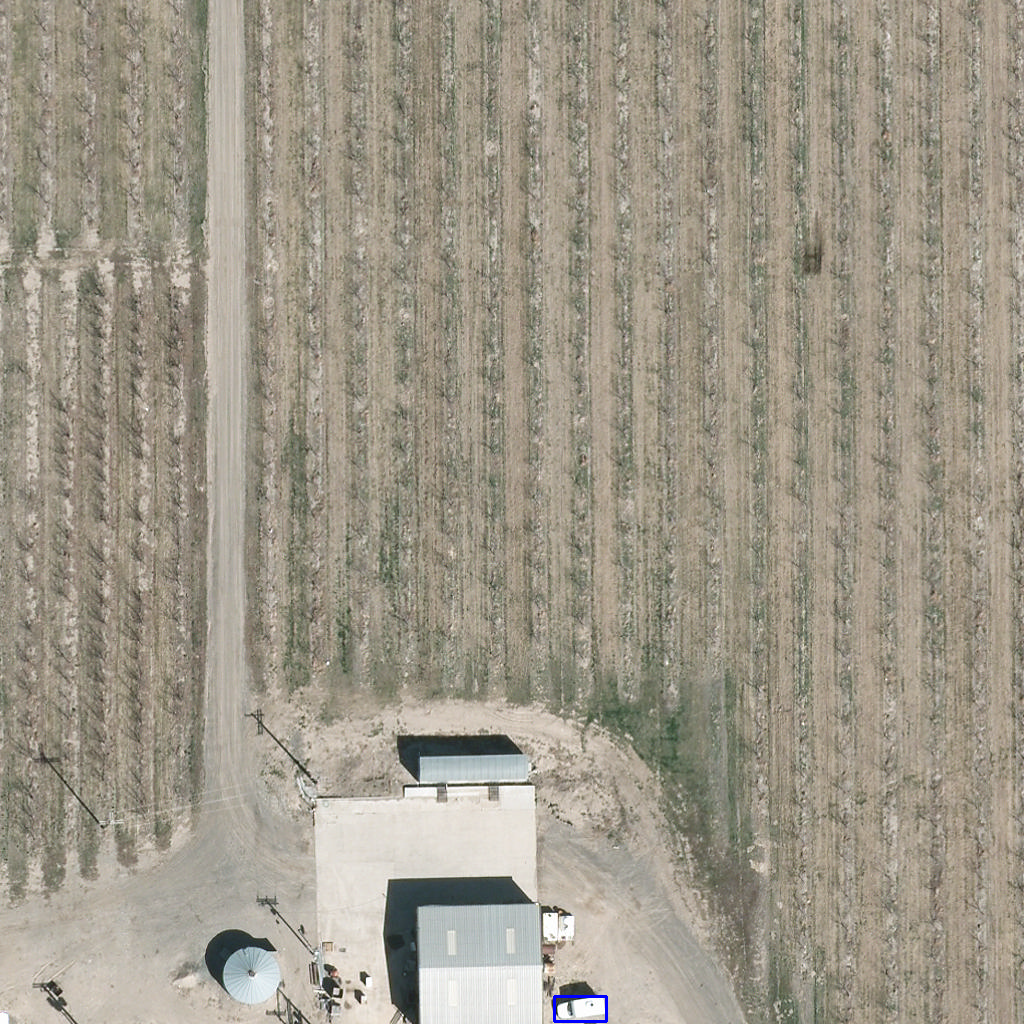
\includegraphics[trim={550pt 0pt 410pt 990pt},clip,width=\textwidth]{images/015Results/01abb_vs_obb/abb_truck.png}
        \caption{Label: "Truck", abb format, area: $\approx 1378 \text{px}$}
        \label{fig:abb_truck}
    \end{subfigure}
    \hfill
    \begin{subfigure}[b]{0.45\textwidth}
        \centering
        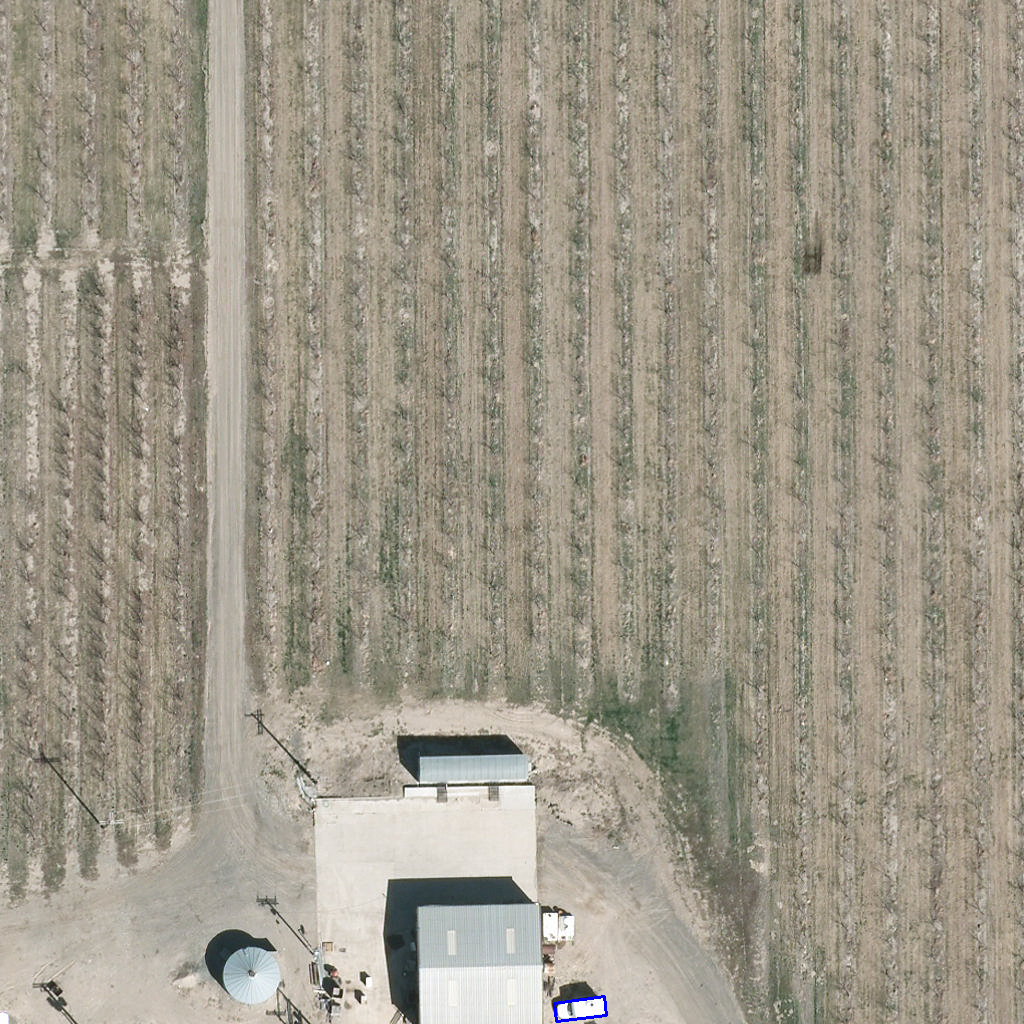
\includegraphics[trim={550pt 0pt 410pt 990pt},clip,width=\textwidth]{images/015Results/01abb_vs_obb/obb_truck.png}
        \caption{Label: "Truck", obb format, area: $\approx 967 \text{px}$}
        \label{fig:obb_truck}
    \end{subfigure}
    
    \vspace{0.5cm} % Abstand zwischen den Zeilen
    
    % Zweite Zeile
    \begin{subfigure}[b]{0.45\textwidth}
        \centering
        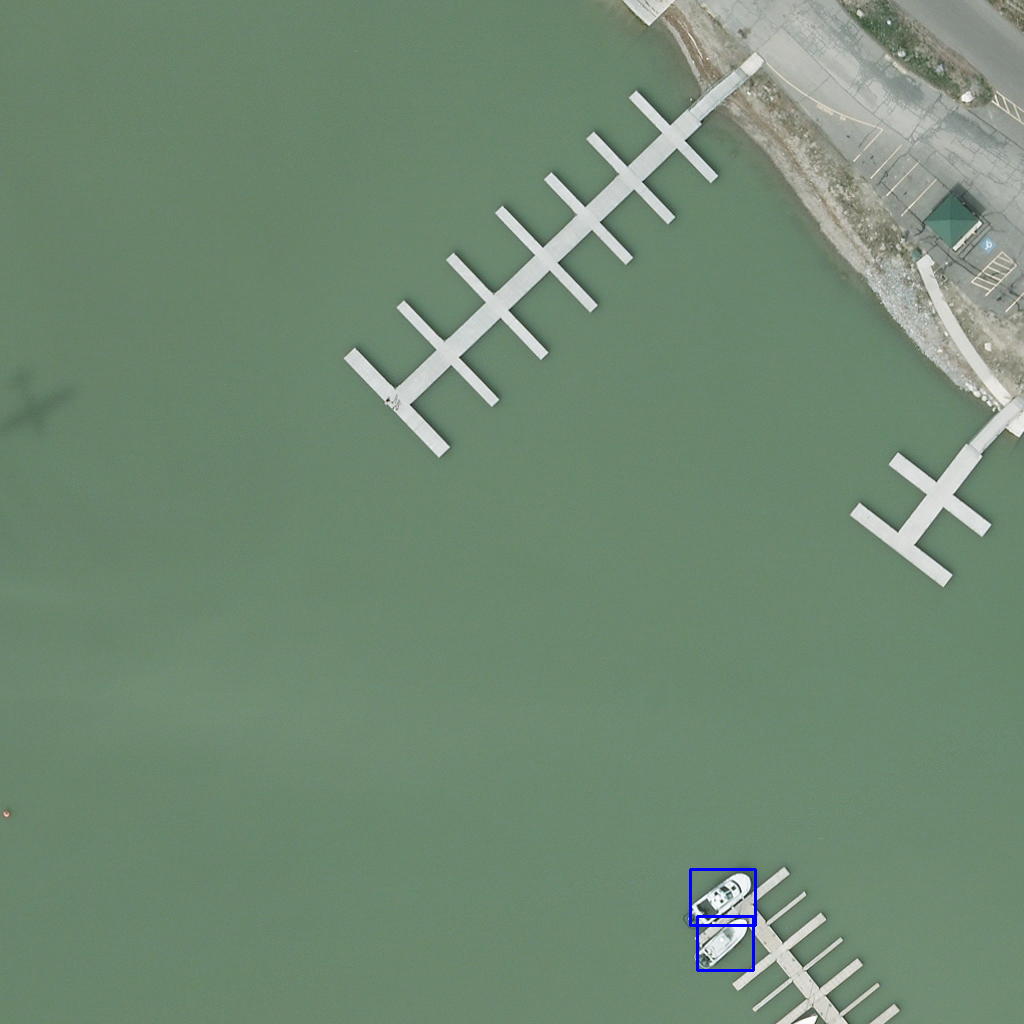
\includegraphics[trim={680pt 50pt 250pt 865pt},clip,width=\textwidth]{images/015Results/01abb_vs_obb/abb_ship.png}
        \caption{Labels: "Ship", abb format}
        \label{fig:abb_ship}
    \end{subfigure}
    \hfill
    \begin{subfigure}[b]{0.45\textwidth}
        \centering
        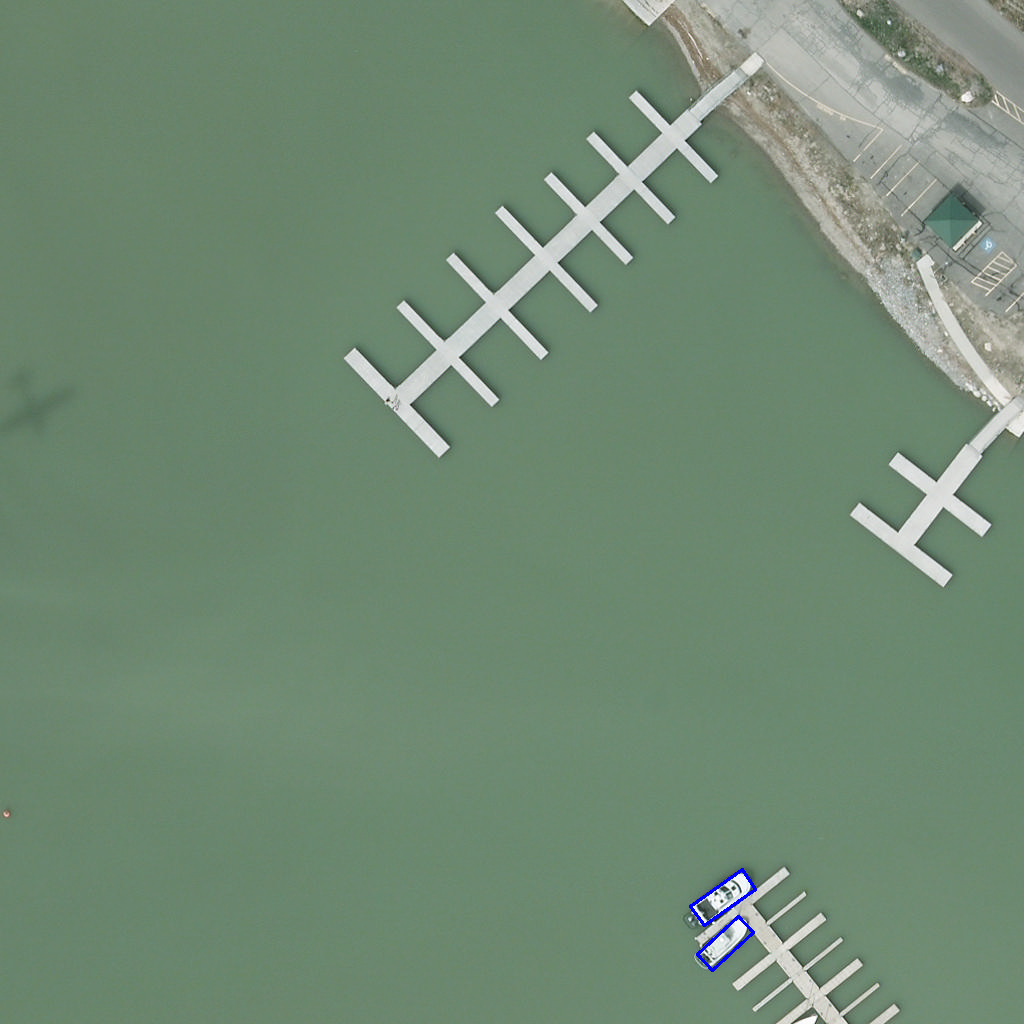
\includegraphics[trim={680pt 50pt 250pt 865pt},clip,width=\textwidth]{images/015Results/01abb_vs_obb/obb_ship.png}
        \caption{Labels: "Ship", obb format}
        \label{fig:obb_ship}
    \end{subfigure}  
    \caption[Comparison of the bounding box formats of two different object classes]{Comparison of the bounding box formats of two different object classes (for full-sized images see \ref{fig:comparison_bb_format_fs})}
    \label{fig:comparison_bb_format}
\end{figure}
\todo{nicht nur erläutern was man sieht sondern auch was man daraus folgert (analyse) im Bildunterschrift}


In Abbildung \ref{fig:comparison_bb_format} wird ein Vergleich zwischen \acrshort{obb} und \acrshort{abb} für verschiedene Objektklassen dargestellt. Besonders deutlich wird dieser Unterschied beim LKW-Beispiel: In Abbildung \ref{fig:abb_truck} nimmt die \acrshort{abb} mit ca. 1378 px eine deutlich größere Fläche ein als die \acrshort{obb} in Abbildung \ref{fig:obb_truck} mit ca. 967 px. Beim Vergleich stark rotierten Objekten, wie etwa bei den Schiffen in Abbildung \ref{fig:abb_ship} und \ref{fig:obb_ship}, zeigt sich, dass die \acrshort{obb} das Objekt selbst deutlich präziser umschließt und weniger umliegendes Areal einbezieht. Ein weiterer Vorteil der \acrshort{obb} ist das Fehlen von Überlappungen zwischen den Boxen. Für weitere Beispiele s. Abb. \ref{fig:aab_obb_example_pics}.

Ein Vergleich aller Bounding Box-Flächen (vgl. Abbildung \ref{fig:bbox_area}) verdeutlicht, dass \acrshort{obb} im Mittel kompakter ist (Median \acrshort{abb}: ca. 1000 px, Median \acrshort{obb}: >700 px). Die \acrshort{abb}-Flächen entsprechen exakt den "abb in obb", da die Bounding Boxes identisch sind; der einzige Unterschied liegt im trainierten Modell. Die Bounding Boxen nehmen  als \acrshort{obb} (ca. 700 px pro Box) etwa 0,066\% der Gesamtfläche des Bildes ein, als \acrshort{abb} (ca. 1000 px pro Box) etwa 0,095\%. Damit liegen \acrshort{obb} knapp unterhalb der Untergrenze für sehr kleine Objekte nach \citeauthor{Chen2017} \cite{Chen2017} (s. Kap. \ref{ch:state_of_research}) und gelten als "very small objects", während \acrshort{abb} oberhalb der Untergrenze für kleine Objekte liegt und damit als "small object" gilt.


% \begin{itemize}
%     \item Zu sehen sind in Fig. \ref{fig:comparison_bb_format} ein Vergleich zwischen \acrshort{obb} und \acrshort{abb} bei verschiedenen Klassen
%     \item Fig. \ref{fig:abb_truck} hat mit ca. 1378 px als \Acrlong{abb} einen deutlich größere Fläche als die in \ref{fig:obb_truck} mit ca. 967 px
%     \item insbesondere beim vergleich der deutlich stärker rotierten \acrshort{BB} bei \ref{fig:obb_ship} und \ref{fig:abb_ship} ist zu sehen, dass die \acrshort{obb} sich deutlich stärker auf das Objekt selbst konzentriert und weniger umgebendes Areal umrandet. Ein weiterer wichtiger Punkt ist, dass keine Überlapppungen bei den \acrshortpl{obb} vorhanden ist.
%     \item  wenn man nun alle Bounding Box Areas vergleicht (s. Fig. \ref{fig:bbox_area}) ist zu sehen, dass obb deutlich kompatker (Median abb: ca. 1000 px, Median obb: >750 px) ist
%     \item \acrshort{abb} ist exakt gleich zu "abb in obb" da die \acrshort{BB} identisch sind ("abb in obb" hat die \acrshort{abb} bounding boxen ohne rotation)"; nur das Trainierte Modell unterscheidet sich
%     \item BB entsprechen der Definition von klein nach \cite{Chen2017}; nehmen als obb (700 px pro Box) ca, 0.066\% der Gesamtfläche des Bildes ein; und als abb (1000 px pro Box) 0.095\%; obb liegt damit knapp unterhalb der Untergrenze (very small object) und abb oberhalb der untergrenze (small object)
% \end{itemize}

\begin{figure}[htbp]
    \centering
    \includesvg[width=0.8\textwidth]{images/015Results/01abb_vs_obb/boxplot_areas.svg}
    \caption[Comparison of Bounding Box Area in pixels for \acrshort{abb}, \acrshort{obb}, abb in obb]{Comparison of Bounding Box Area in pixels for \acrshort{abb}, \acrshort{obb}, abb in obb. "aab in obb" means, that \acrlong{abb} converted to obb was used in the \acrshort{YOLO}v9u model with zero rotation. (Own representation)}
    \label{fig:bbox_area}
\end{figure}


\begin{figure}[htbp]
    \centering
    \includesvg[width=0.8\textwidth]{images/015Results/01abb_vs_obb/abb_obb_best_val_on_val.svg}
    \caption[Comparison of \acrshort{mAP}50-95 values for \acrshort{abb} and \acrshort{obb} (Best validation model on validation dataset)]{Comparison of \acrshort{mAP}50-95 values for \acrshort{abb} and \acrshort{obb} (Best validation model on validation dataset). "aab in obb" means, that \acrlong{abb} converted to obb was used in the \acrshort{YOLO}v9u model with zero rotation. (Own representation)}
    \label{fig:obb_abb_map50-95:val_on_val}
\end{figure}
Die Analyse der \acrshort{mAP}50--95 des besten Validierungsmodells auf dem Validierungsdatensatz (Abbildung \ref{fig:obb_abb_map50-95:val_on_val}) zeigt, dass das \acrshort{obb}-Modell in allen Fällen eine bessere Leistung erzielt als das \acrshort{abb}-Modell. Interessanterweise erzielt \acrshort{abb} auf dem \acrshort{obb}-Modell eine höhere Performance als die angepassten \acrshort{obb}-Boxen innerhalb desselben Modells (yolov9u). Dasselbe Phänomen lässt sich auch auf dem Testdatensatz beobachten (Abbildung \ref{fig:obb_abb_map50-95:val_on_test}), sodass \acrshort{abb} in Verbindung mit dem \acrshort{obb}-Modell bessere Ergebnisse liefert. Auffällig ist, dass bei den \acrshort{abb}-basierten Modellen (sowohl \acrshort{abb} als auch "abb in obb") stets Fold 1 den besten Wert beim Validation Dataset auf dem Validation Dataset erreicht hat, während beim \acrshort{obb}-Modell Fold 0 dort die besten Ergebnisse lieferte (s. Tab. \ref{tab:best_folds_area} und Fig. \ref{fig:obb_abb_map50-95:val_on_val}). Die Ergebnisse der jeweiligen Folds mit dem höchsten \acrshort{mAP}50-95 Wert aus Abb. \ref{fig:obb_abb_map50-95:val_on_val} sind durch den roten Punkt in Abbildung \ref{fig:obb_abb_map50-95:val_on_test} gekennzeichnet. Auffällig ist, dass die meisten roten Punkte im Bereich des Medians der Modelle liegen und lediglich das \acrshort{RGIR}-Modell eine Übereinstimmung zwischen dem besten Fold im Testdatensatz und dem besten Fold im Validierungsdatensatz aufweist. \todo{nächster Satz ist eigentlich analyse (auskommentiert)}
% Die Konsistenz über alle fünf Folds der Kreuzvalidierung ist gut, was auf eine robuste Trainierbarkeit der Modelle hinweist. 

\begin{table}[h]
\centering
\begin{tabular}{l c c}
\hline
\textbf{Model} & \textbf{Best mAP Fold (Validation)} & \textbf{Best mAP Fold (Test)} \\ 
\hline
abb &  1 & 1 \\
obb &  0 & 0 \\
abb in obb &  1 & 1 \\
\hline
\end{tabular}
\caption{Best fold per model at Bounding Box format}
\label{tab:best_folds_area}
\end{table}


Die Auswirkungen der unterschiedlichen Rotationen der erkannten Objekte lassen sich in Abbildung \ref{fig:aab_obb_example_pics} exemplarisch an der Klasse \texttt{plane} beobachten. Die Bounding Boxes unterscheiden sich hinsichtlich ihrer Rotationswinkel deutlich zwischen den drei Modellen. Abweichungen in der Überlappung der erkannten Bounding Boxes mit den Ground-Truth-Annotationen treten hingegen wesentlich seltener auf, was die höhere \acrshort{mAP}-Performance der \acrshort{abb}-basierten Modelle erklärt. Auf weitere Auffälligkeiten, wie die Schwierigkeiten bei der Trennung von Objekten und Hintergrund, wird in den folgenden Abschnitten eingegangen.  

Aufgrund der geringeren Wahrscheinlichkeit für Überlappungsfehler sowie der präziseren Objektumrandung wurde das \acrshort{obb}-Modell für die Durchführung der Permutationstests ausgewählt.

% \begin{itemize}
%     \item Auswirkungen der verschiedenen Rotationen der erkanntne Objekte kann man gut in Abb \ref{fig:aab_obb_example_pics} bei \texttt{plane} seehn, die BBs unterscheiden sich in der Rotation zwischen allen 3 Modellen stark. Abweichungen bei der Überlappung der erkannten abbs mit dem Ground Truth abb sind deutlich seltener, was eine höhere map performance erklärt. Auf die weiteren Auffälligkeitne, wie die Schwierigkeiten bei Objekt-Hintergrund Unterscheidung, wird in den nächsten Abschnitten eingegangen.
% \end{itemize}

\begin{figure}[h!]
\centering
\renewcommand{\arraystretch}{1.2} % mehr Platz zwischen Zeilen
\setlength{\tabcolsep}{2pt} % weniger Platz zwischen Spalten
\begin{tabularx}{\textwidth}{c|*{9}{X}}
    & \textbf{Car}
    & \textbf{Truck}
    & \textbf{Camping Car}
    & \textbf{Tractor}
    & \textbf{Plane}
    & \textbf{Ship}
    & \textbf{Vehicle}
    & \textbf{Pick-Up}
    & \textbf{Van} \\ \hline
    \rotatebox{90}{\textbf{\acrshort{GT} (\acrshort{abb})}} 
    %Car
    & 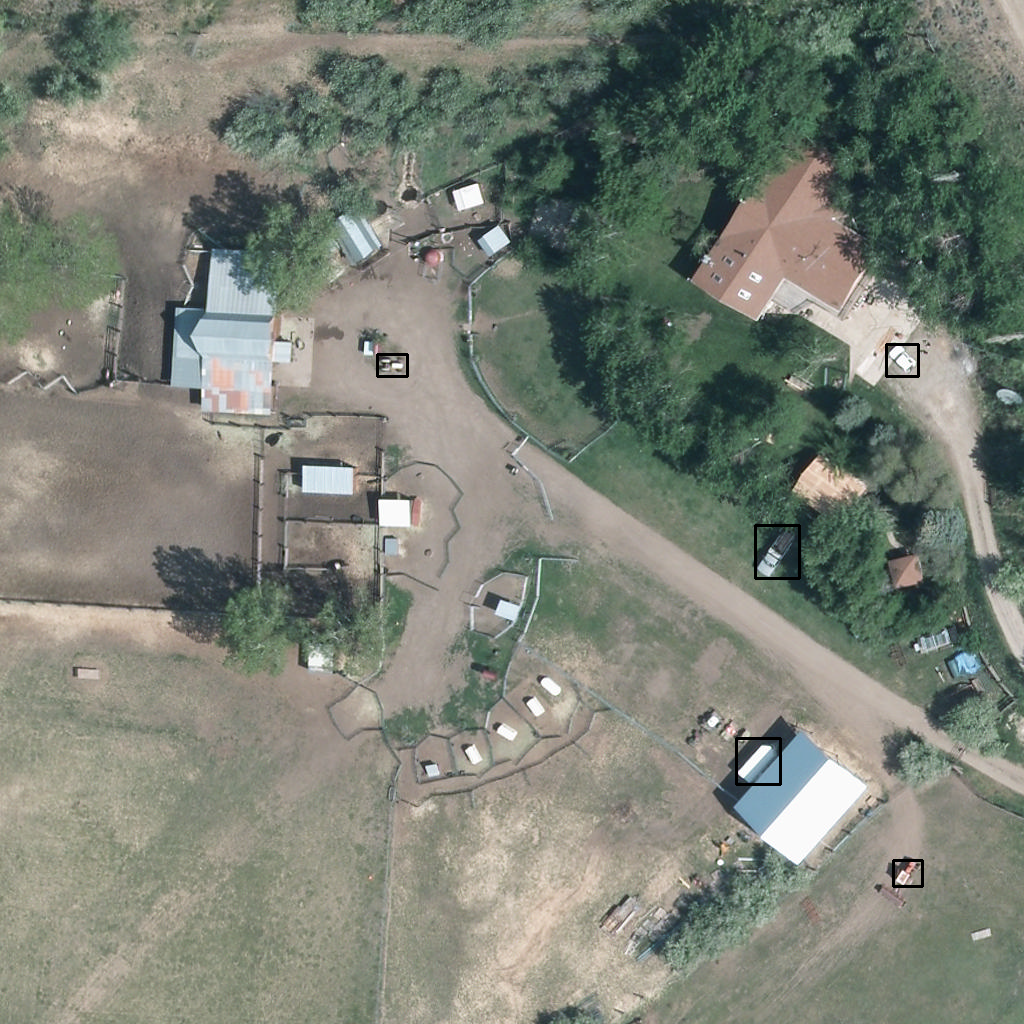
\includegraphics[trim={880pt 630pt 70pt 330pt},clip,width=\linewidth]{images/015Results/01abb_vs_obb/comp_images/ground_truth_abb/523.png}
    %Truck
    & 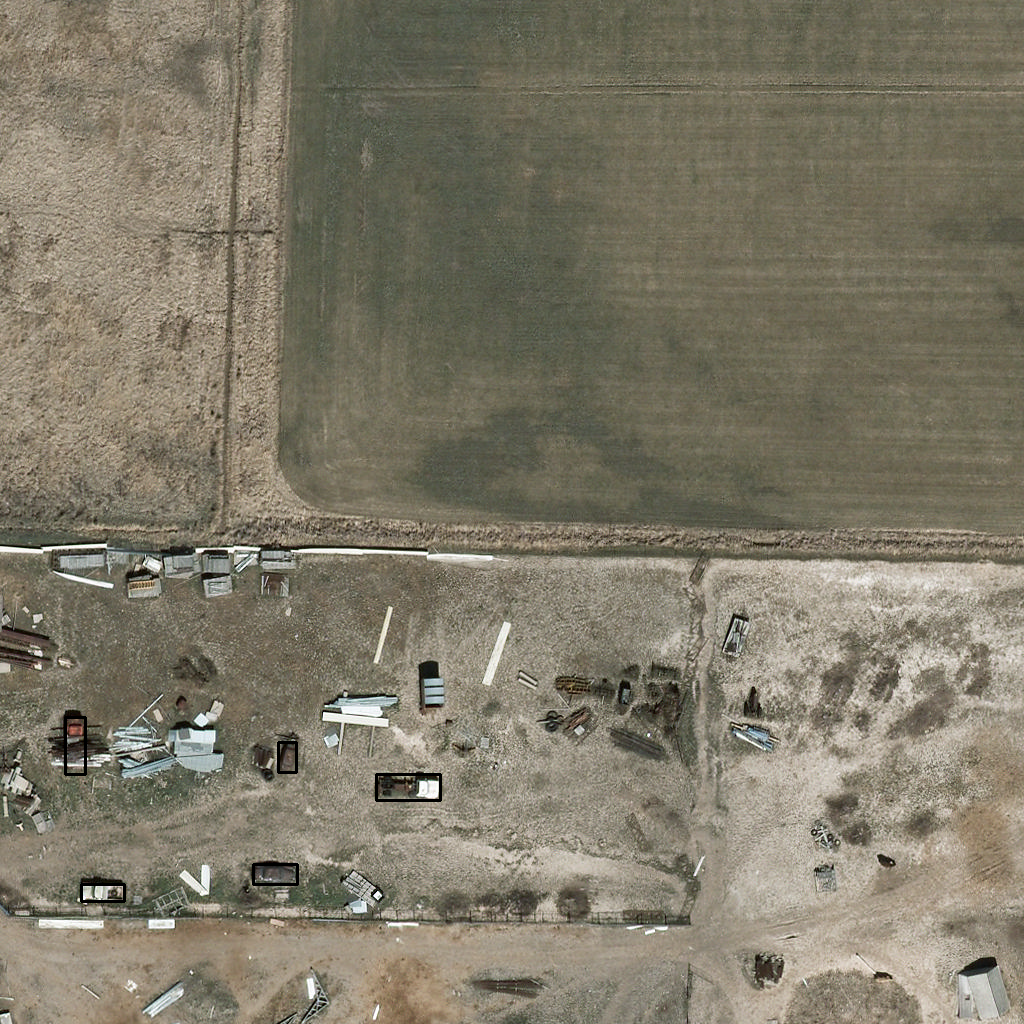
\includegraphics[trim={360pt 200pt 540pt 715pt},clip,width=\linewidth]{images/015Results/01abb_vs_obb/comp_images/ground_truth_abb/212.png}
    %Camping Car
    & 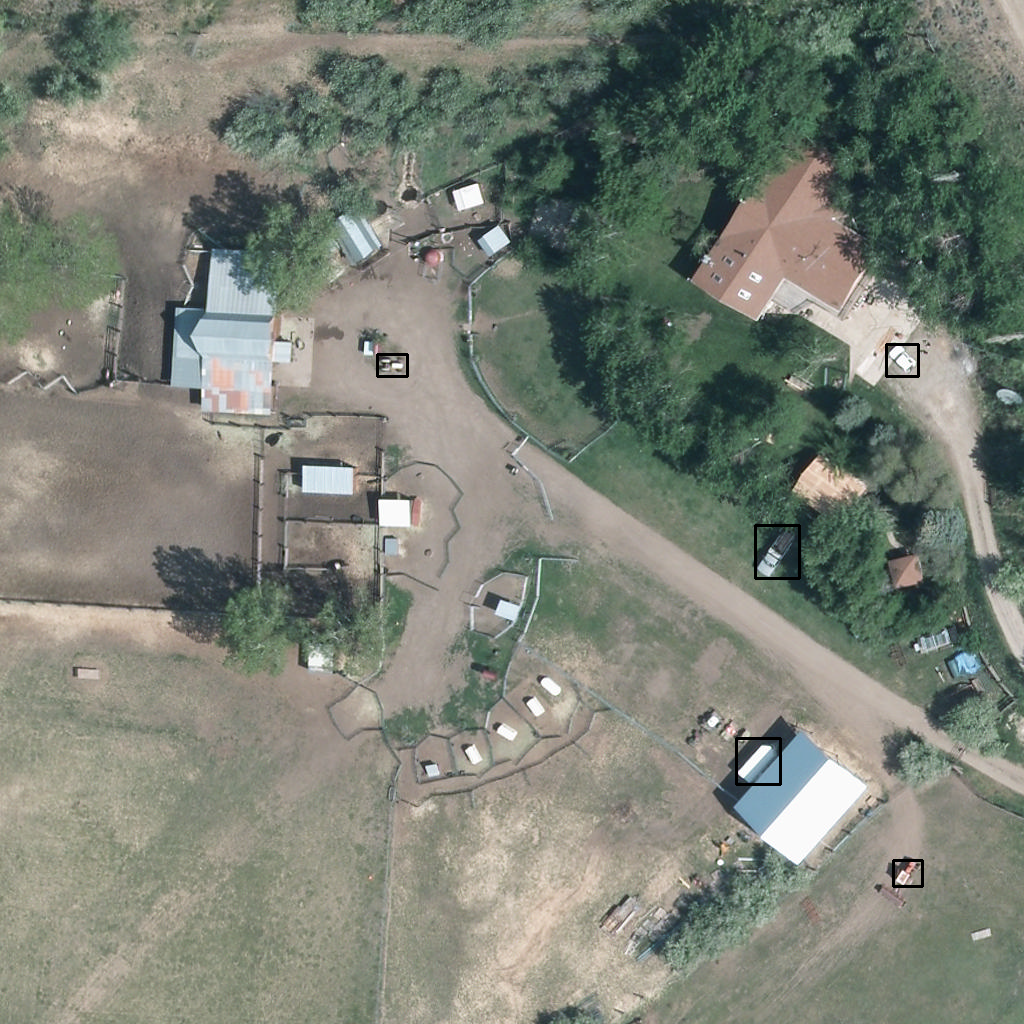
\includegraphics[trim={730pt 220pt 200pt 720pt},clip,width=\linewidth]{images/015Results/01abb_vs_obb/comp_images/ground_truth_abb/523.png}
    %Tractor
    & 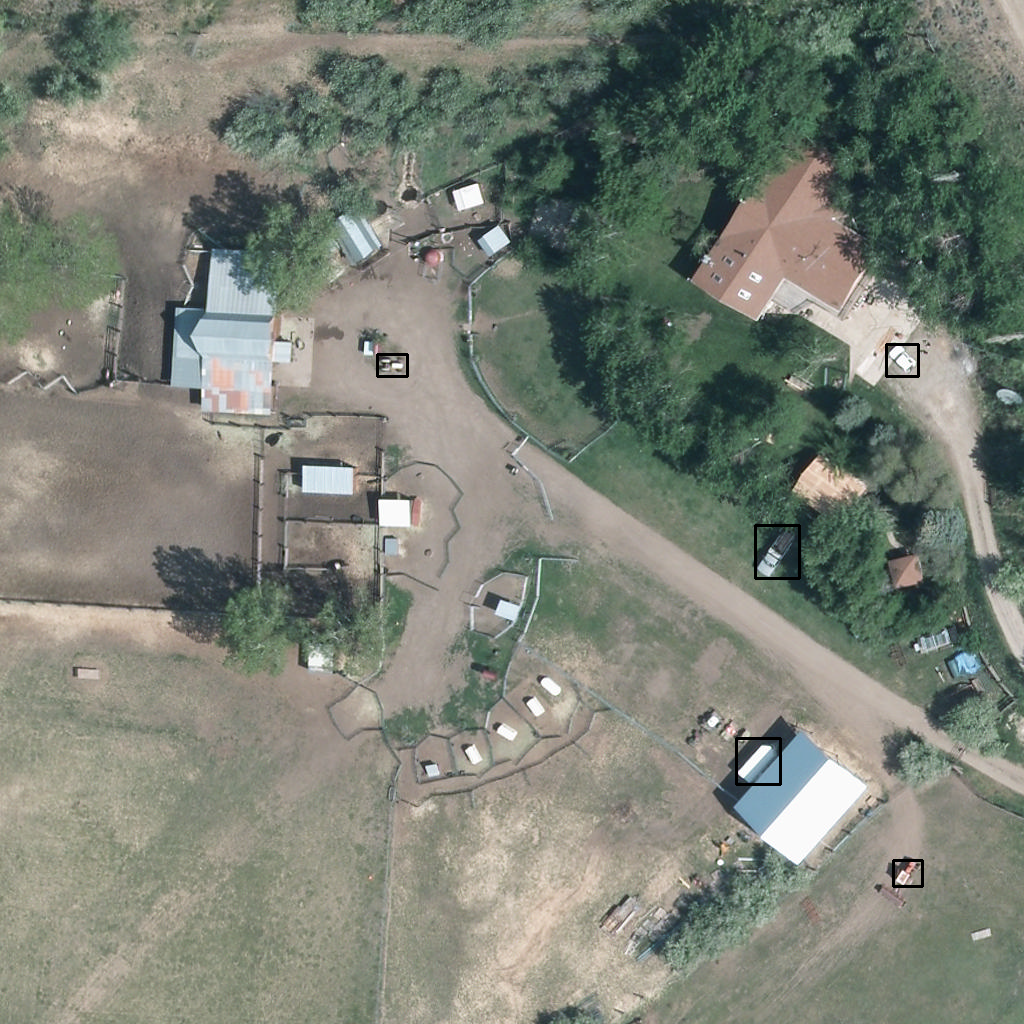
\includegraphics[trim={850pt 110pt 80pt 830pt},clip,width=\linewidth]{images/015Results/01abb_vs_obb/comp_images/ground_truth_abb/523.png}
    %Plane
    &  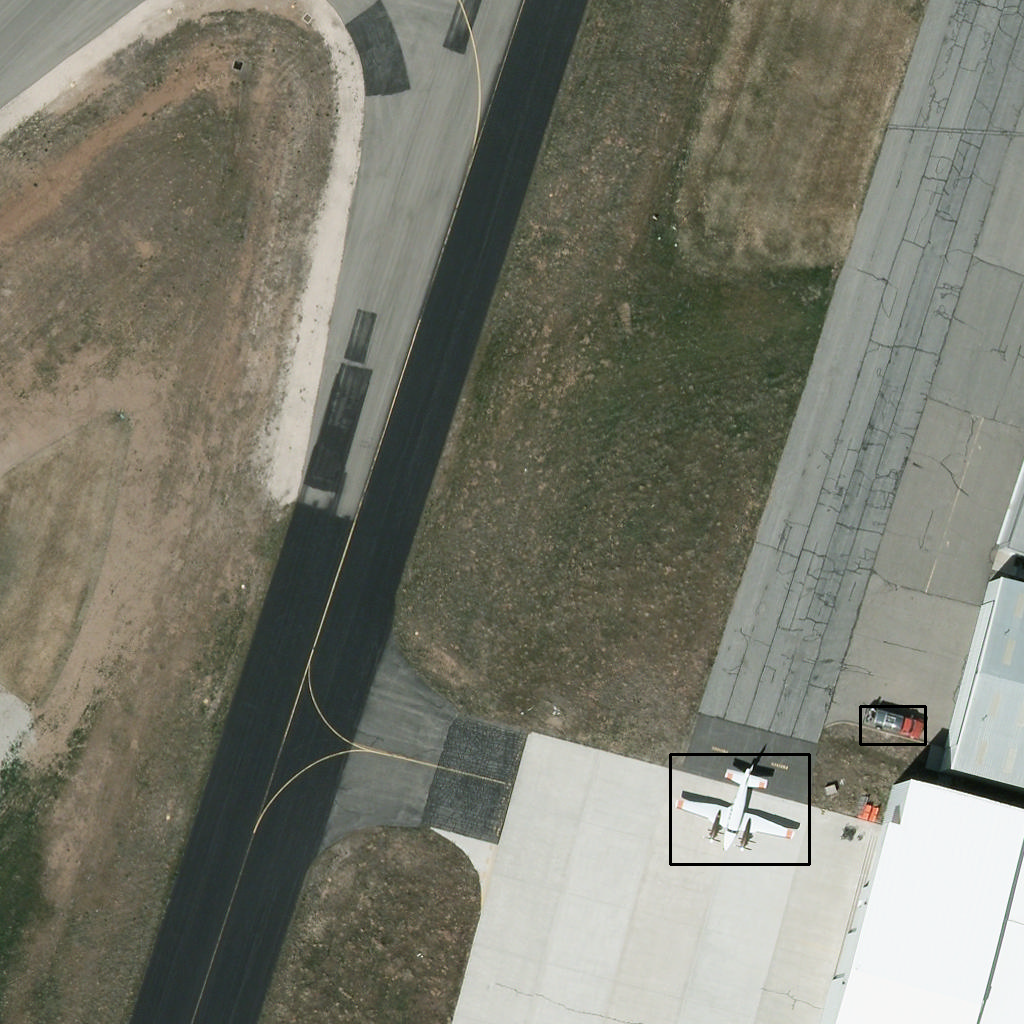
\includegraphics[trim={650pt 120pt 170pt 720pt},clip,width=\linewidth]{images/015Results/01abb_vs_obb/comp_images/ground_truth_abb/487.png}
    %Ship
    & 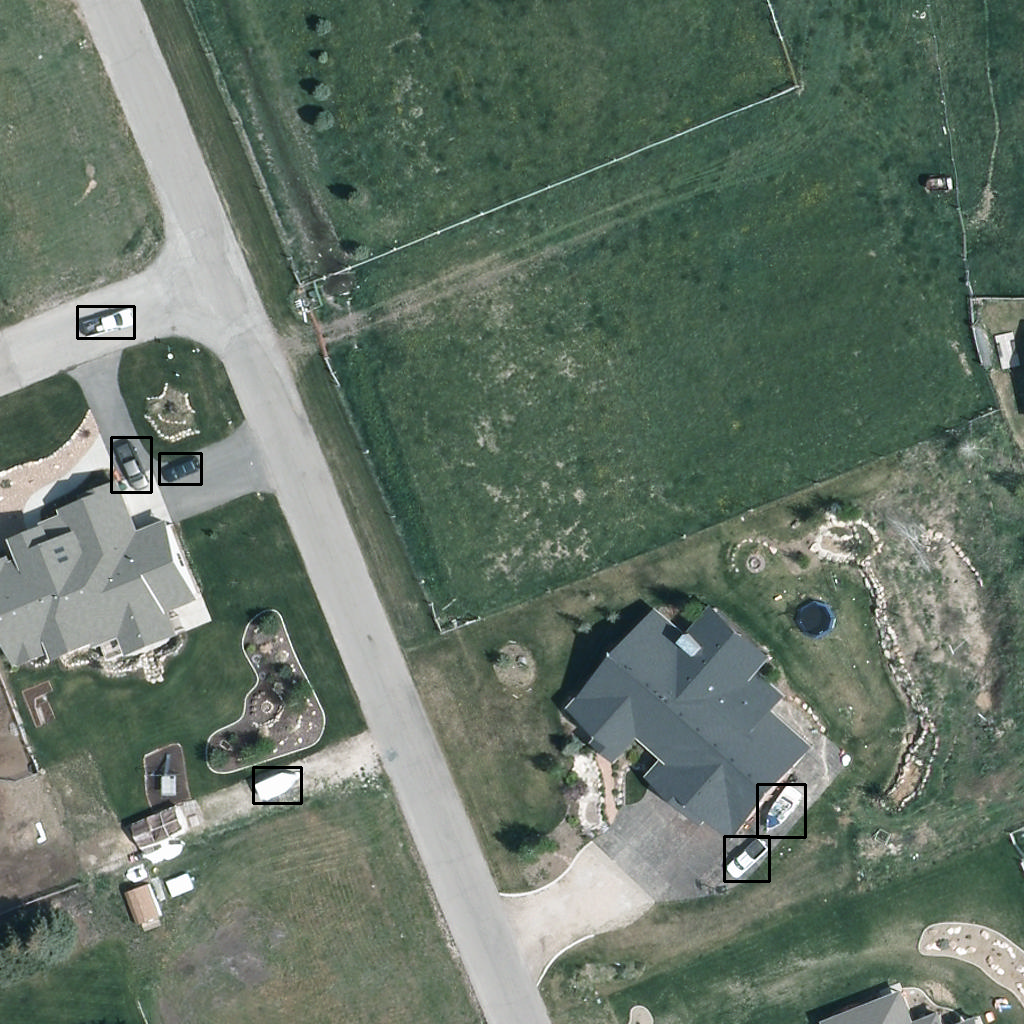
\includegraphics[trim={230pt 200pt 680pt 725pt},clip,width=\linewidth]{images/015Results/01abb_vs_obb/comp_images/ground_truth_abb/509.png}
    %vehicle
    & 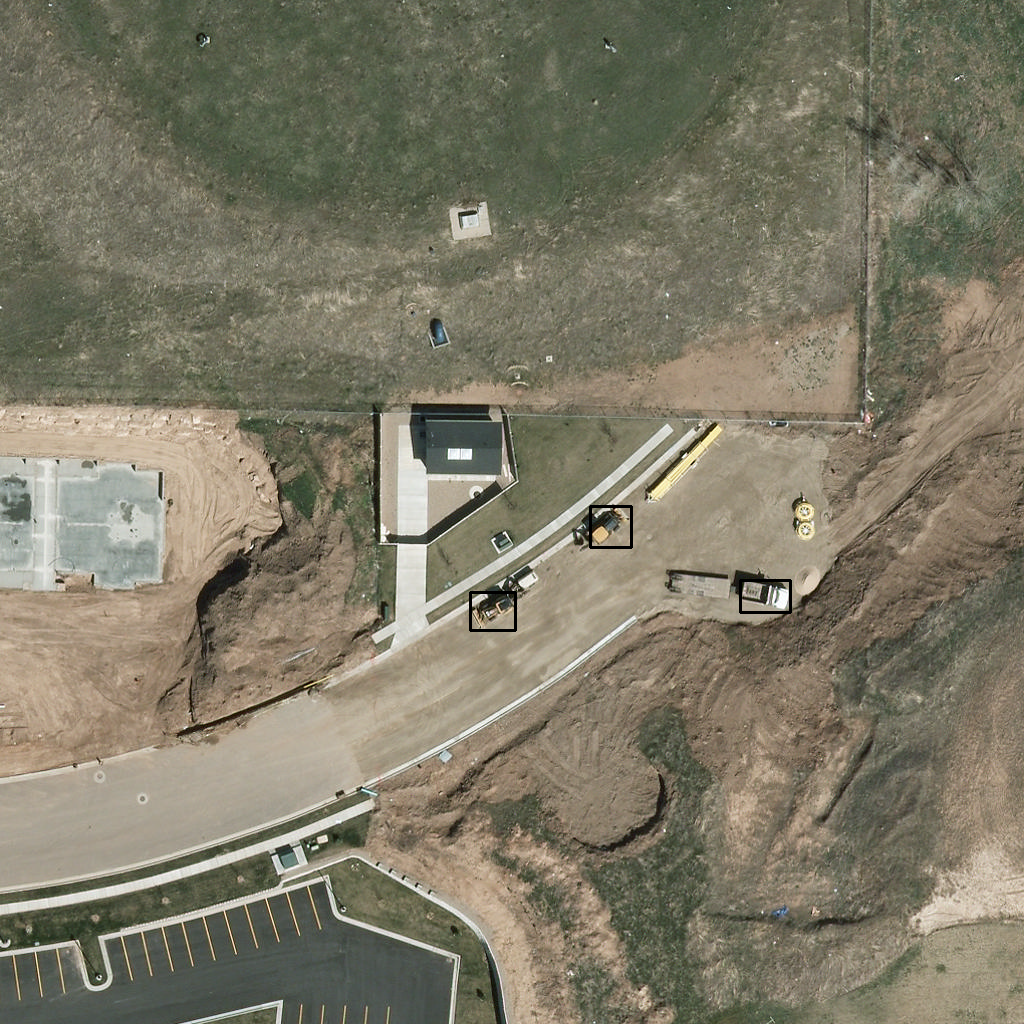
\includegraphics[trim={440pt 360pt 460pt 555pt},clip,width=\linewidth]{images/015Results/01abb_vs_obb/comp_images/ground_truth_abb/427.png}
    %Pick Up
    & 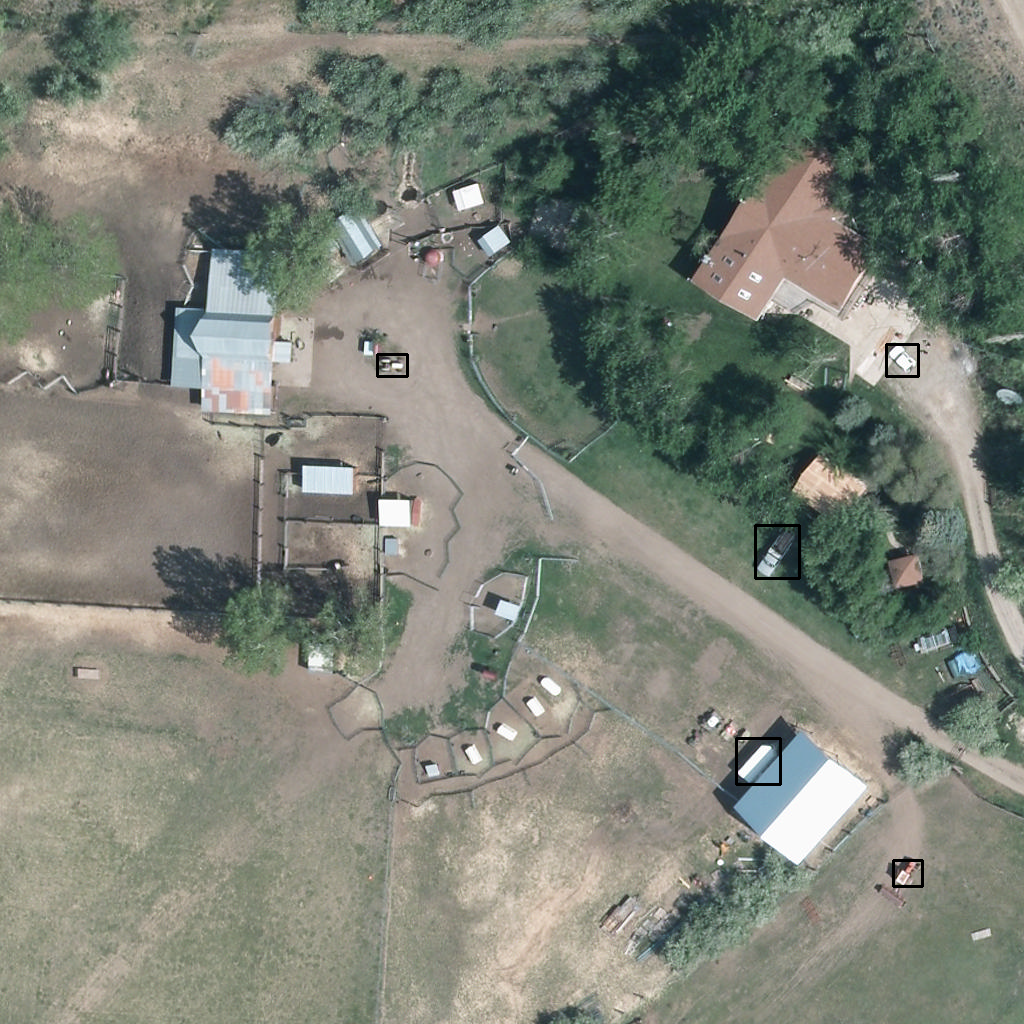
\includegraphics[trim={740pt 420pt 180pt 510pt},clip,width=\linewidth]{images/015Results/01abb_vs_obb/comp_images/ground_truth_abb/523.png}
    %Van
    & 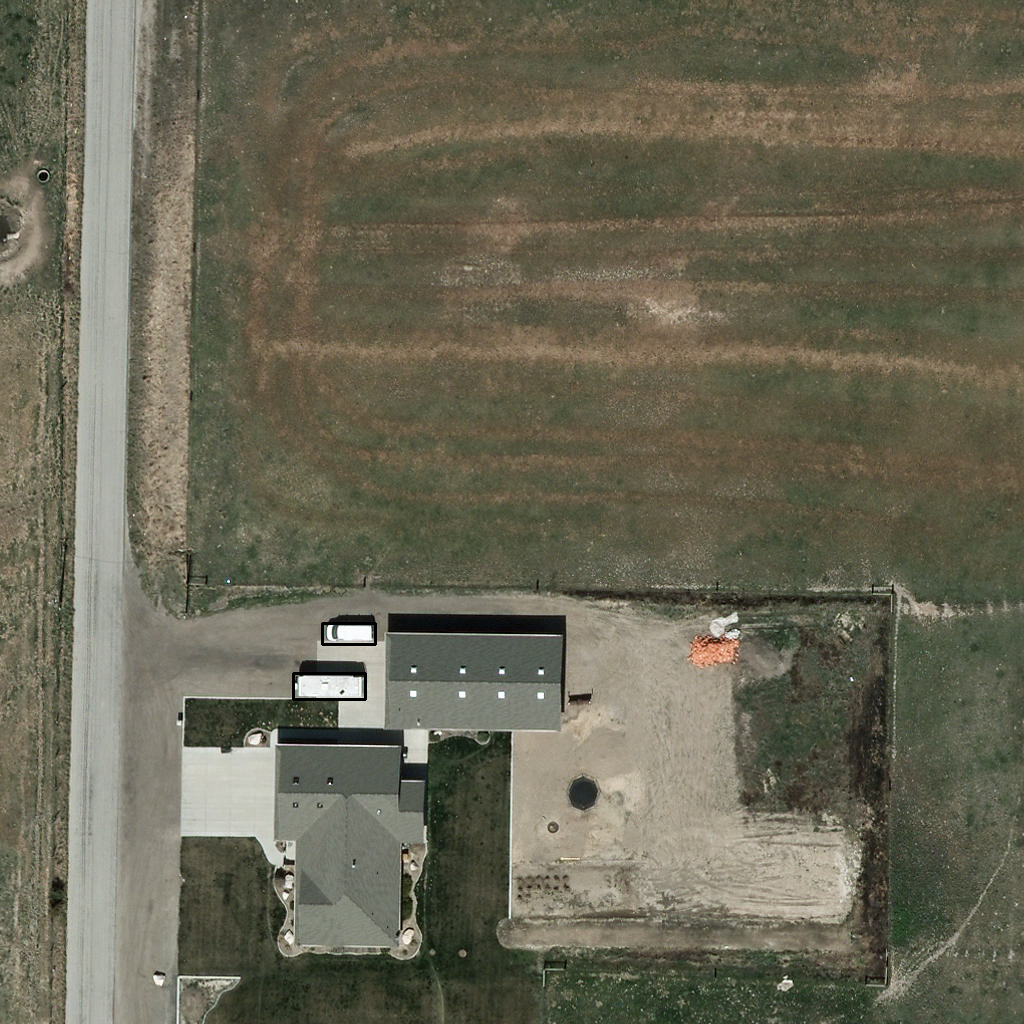
\includegraphics[trim={300pt 355pt 610pt 570pt},clip,width=\linewidth]{images/015Results/01abb_vs_obb/comp_images/ground_truth_abb/198.png} \\ \hline

    \rotatebox{90}{\textbf{\acrshort{GT} (\acrshort{obb})}} 
    %Car
    & 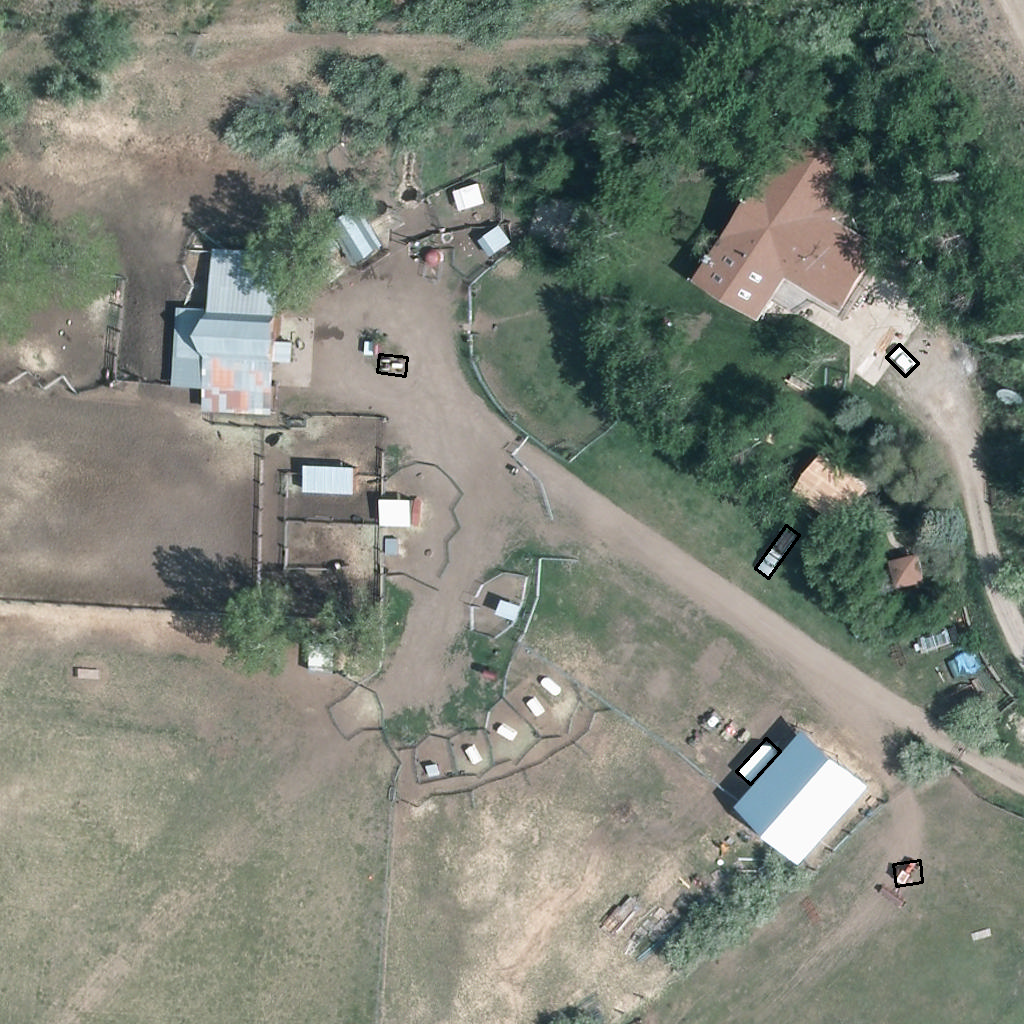
\includegraphics[trim={880pt 630pt 70pt 330pt},clip,width=\linewidth]{images/015Results/01abb_vs_obb/comp_images/ground_truth_obb/523.png}
    %Truck
    & 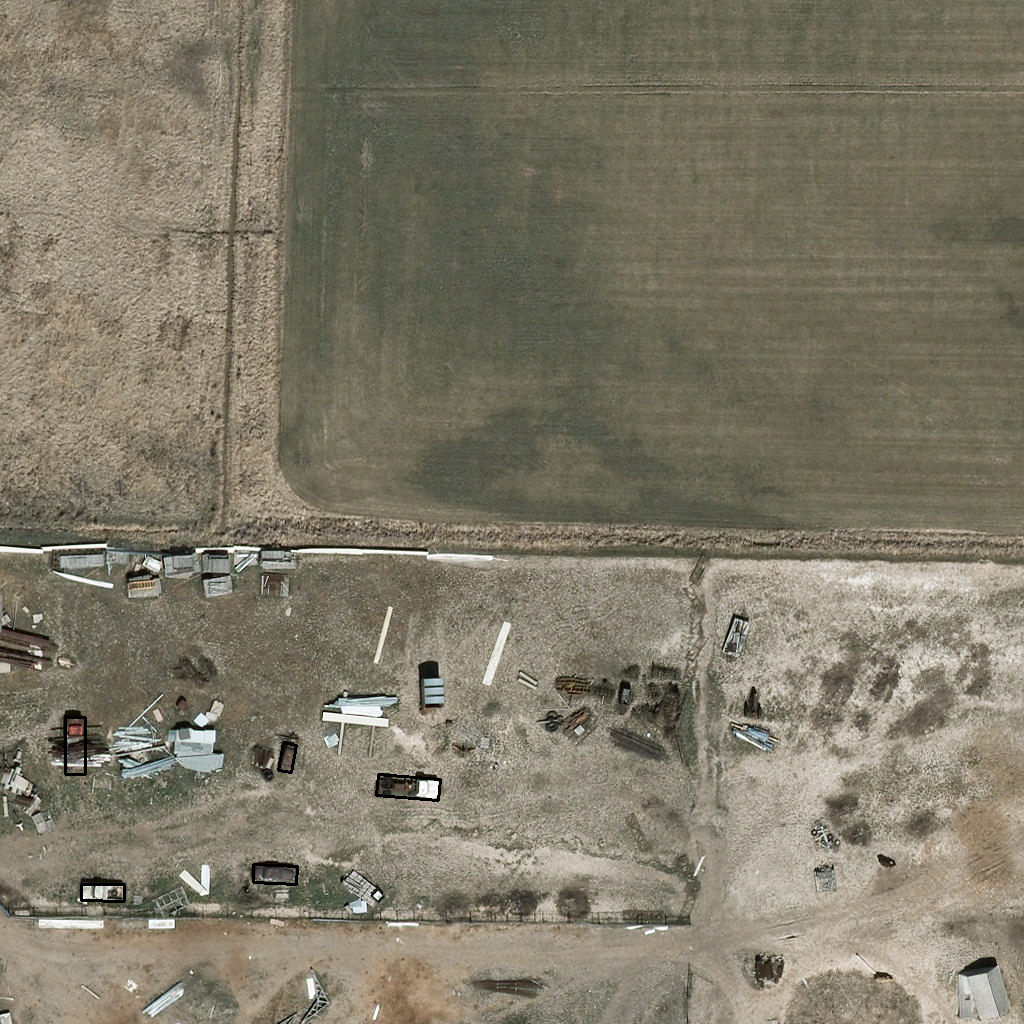
\includegraphics[trim={360pt 200pt 540pt 715pt},clip,width=\linewidth]{images/015Results/01abb_vs_obb/comp_images/ground_truth_obb/212.png}
    %Camping Car
    & 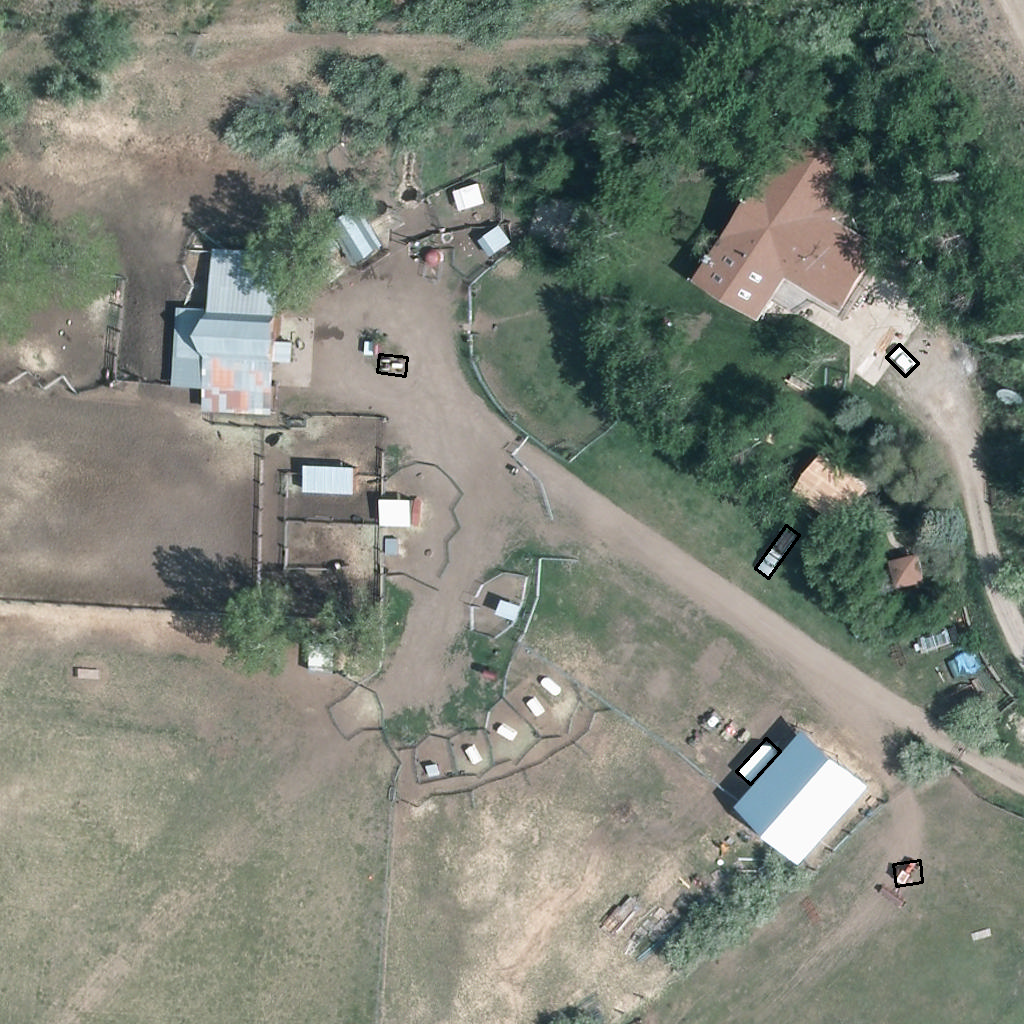
\includegraphics[trim={730pt 220pt 200pt 720pt},clip,width=\linewidth]{images/015Results/01abb_vs_obb/comp_images/ground_truth_obb/523.png}
    %Tractor
    & 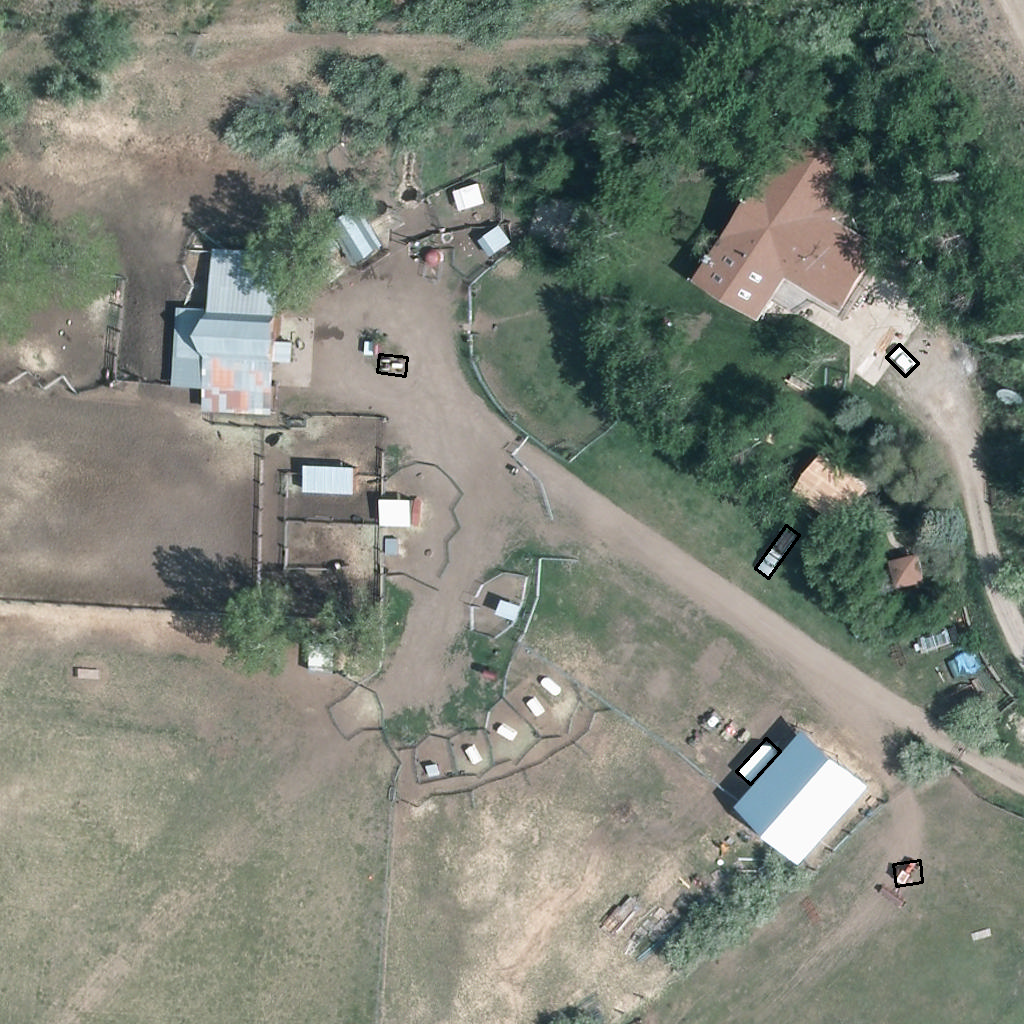
\includegraphics[trim={850pt 110pt 80pt 830pt},clip,width=\linewidth]{images/015Results/01abb_vs_obb/comp_images/ground_truth_obb/523.png}
    %Plane
    &  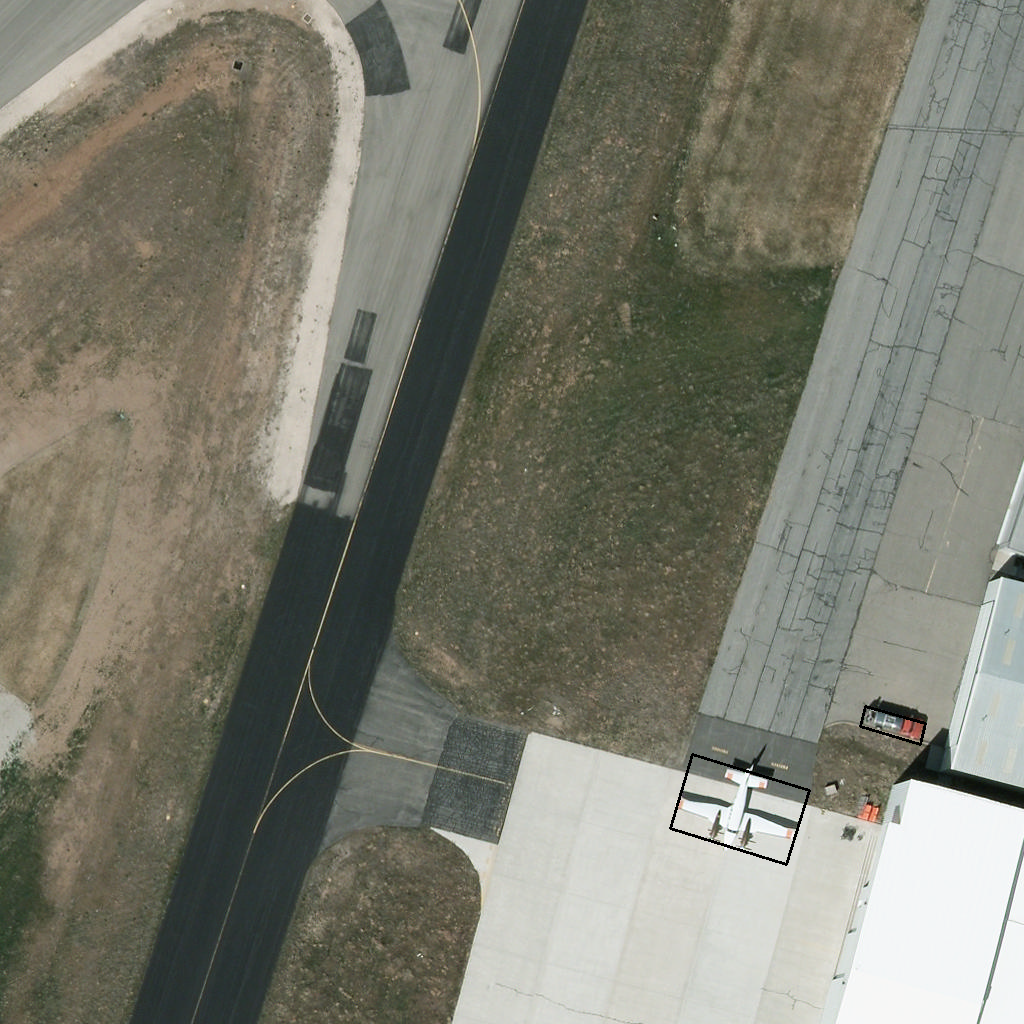
\includegraphics[trim={650pt 120pt 170pt 720pt},clip,width=\linewidth]{images/015Results/01abb_vs_obb/comp_images/ground_truth_obb/487.png}
    %Ship
    & 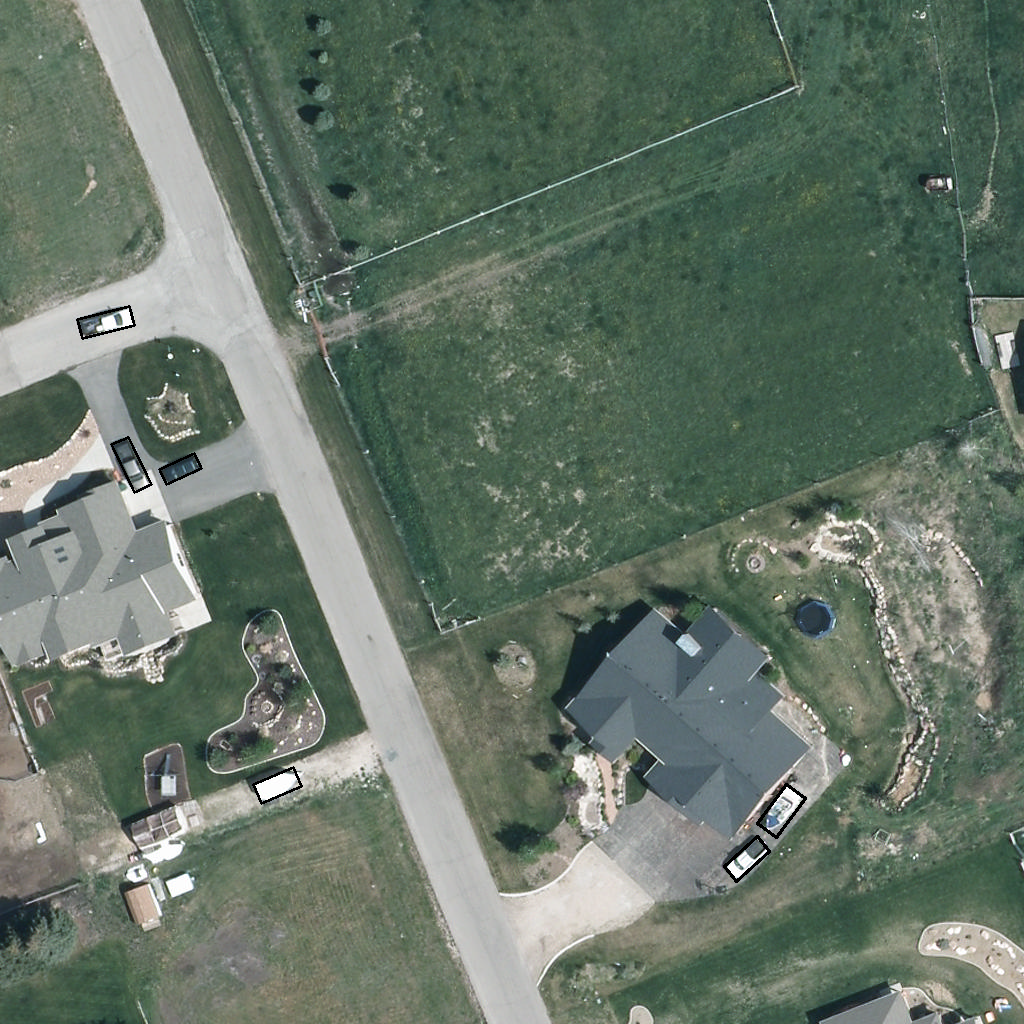
\includegraphics[trim={230pt 200pt 680pt 725pt},clip,width=\linewidth]{images/015Results/01abb_vs_obb/comp_images/ground_truth_obb/509.png}
    %vehicle
    & 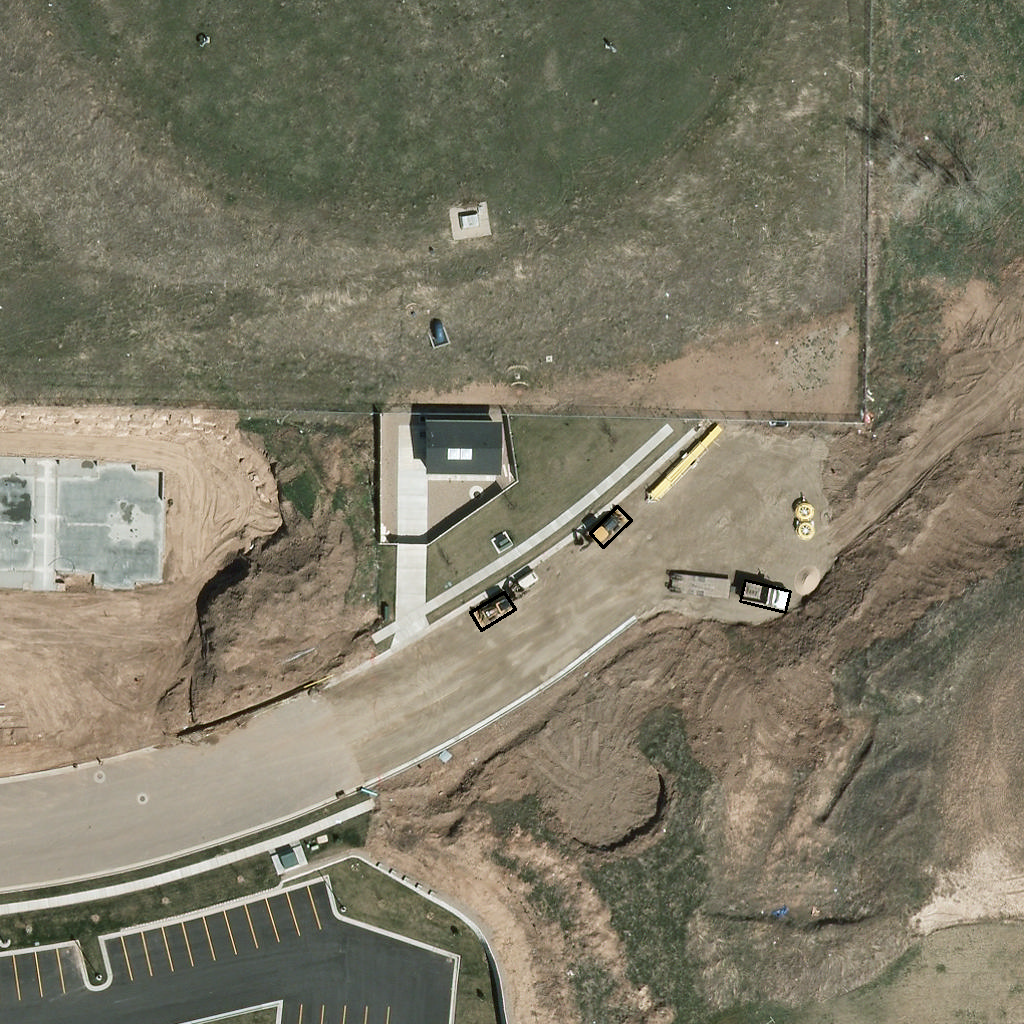
\includegraphics[trim={440pt 360pt 460pt 555pt},clip,width=\linewidth]{images/015Results/01abb_vs_obb/comp_images/ground_truth_obb/427.png}
    %Pick Up
    & 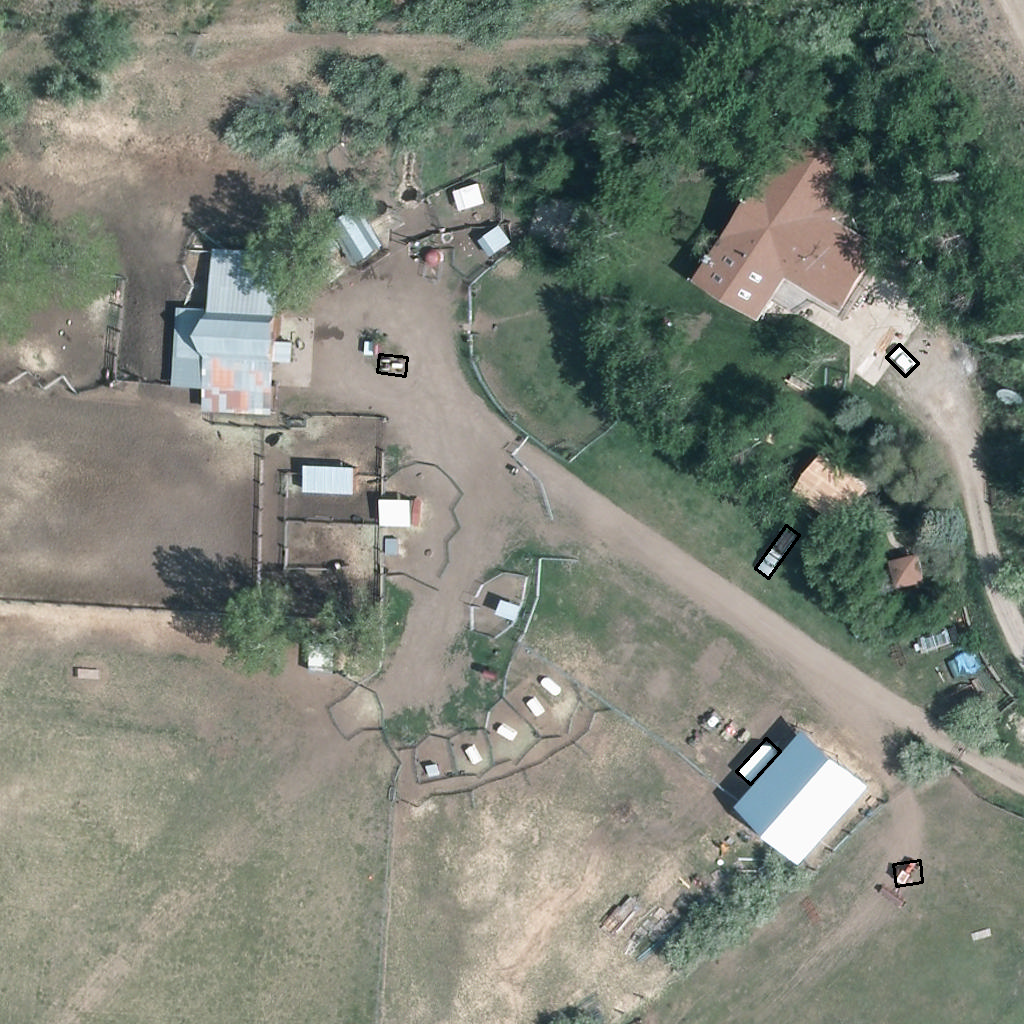
\includegraphics[trim={740pt 420pt 180pt 510pt},clip,width=\linewidth]{images/015Results/01abb_vs_obb/comp_images/ground_truth_obb/523.png}
    %Van
    & 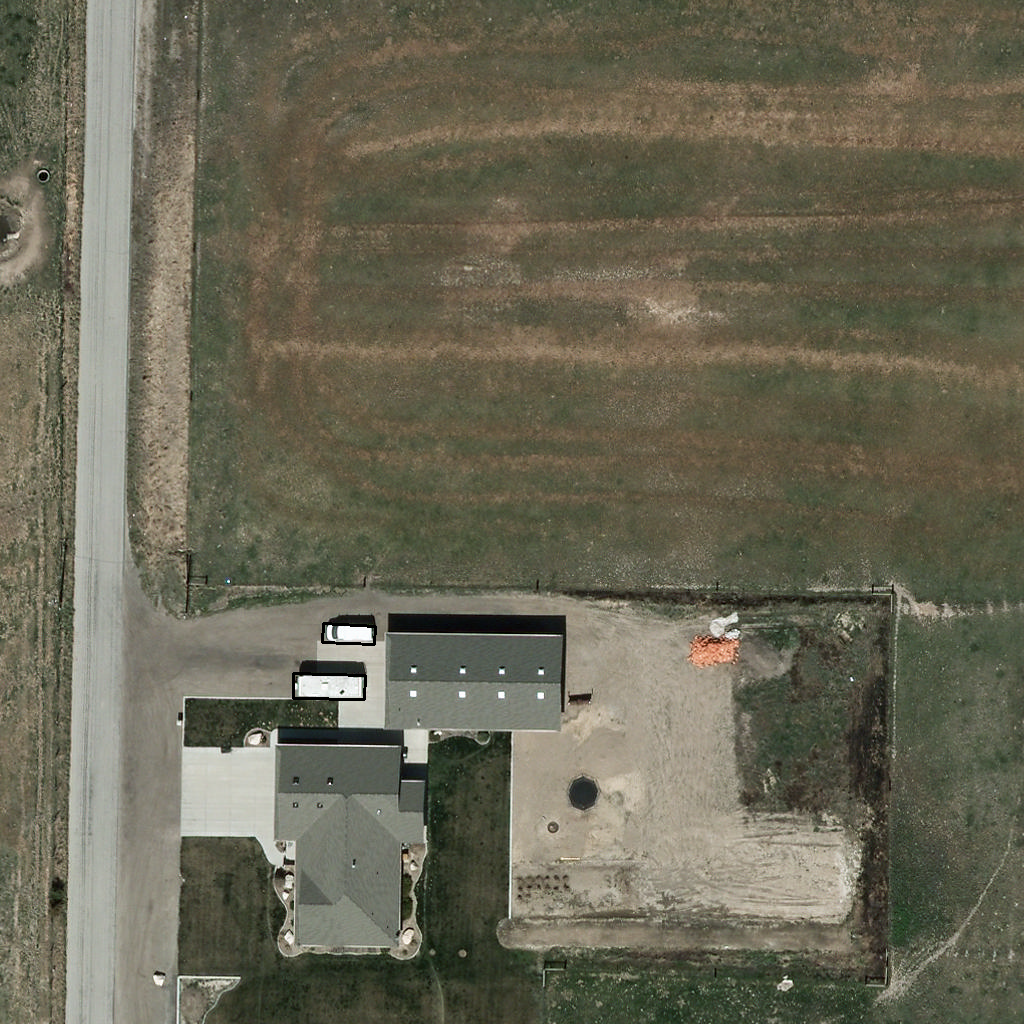
\includegraphics[trim={300pt 355pt 610pt 570pt},clip,width=\linewidth]{images/015Results/01abb_vs_obb/comp_images/ground_truth_obb/198.png} \\ \hline
    \rotatebox{90}{\textbf{\acrshort{abb}}} 
    %Car
    & 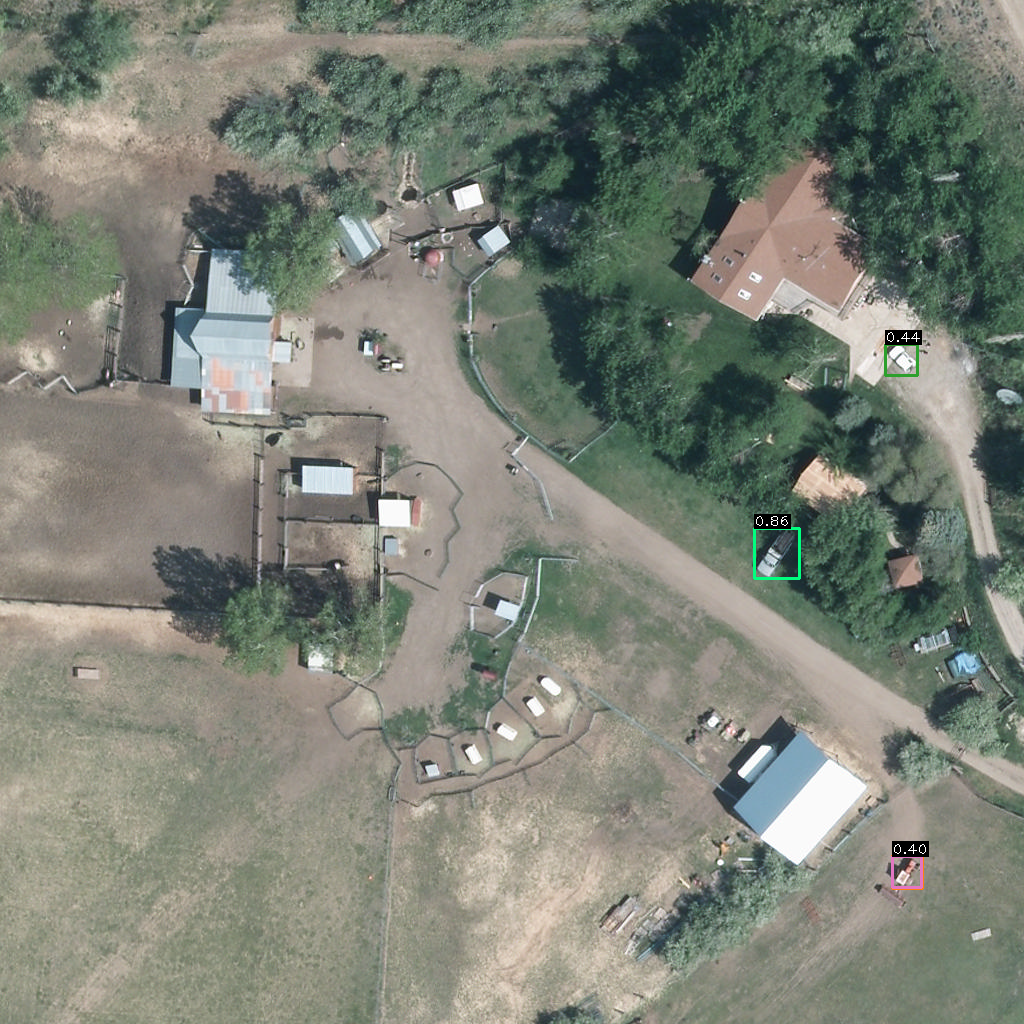
\includegraphics[trim={880pt 630pt 70pt 330pt},clip,width=\linewidth]{images/015Results/01abb_vs_obb/comp_images/abb/523.png}
    %Truck
    & 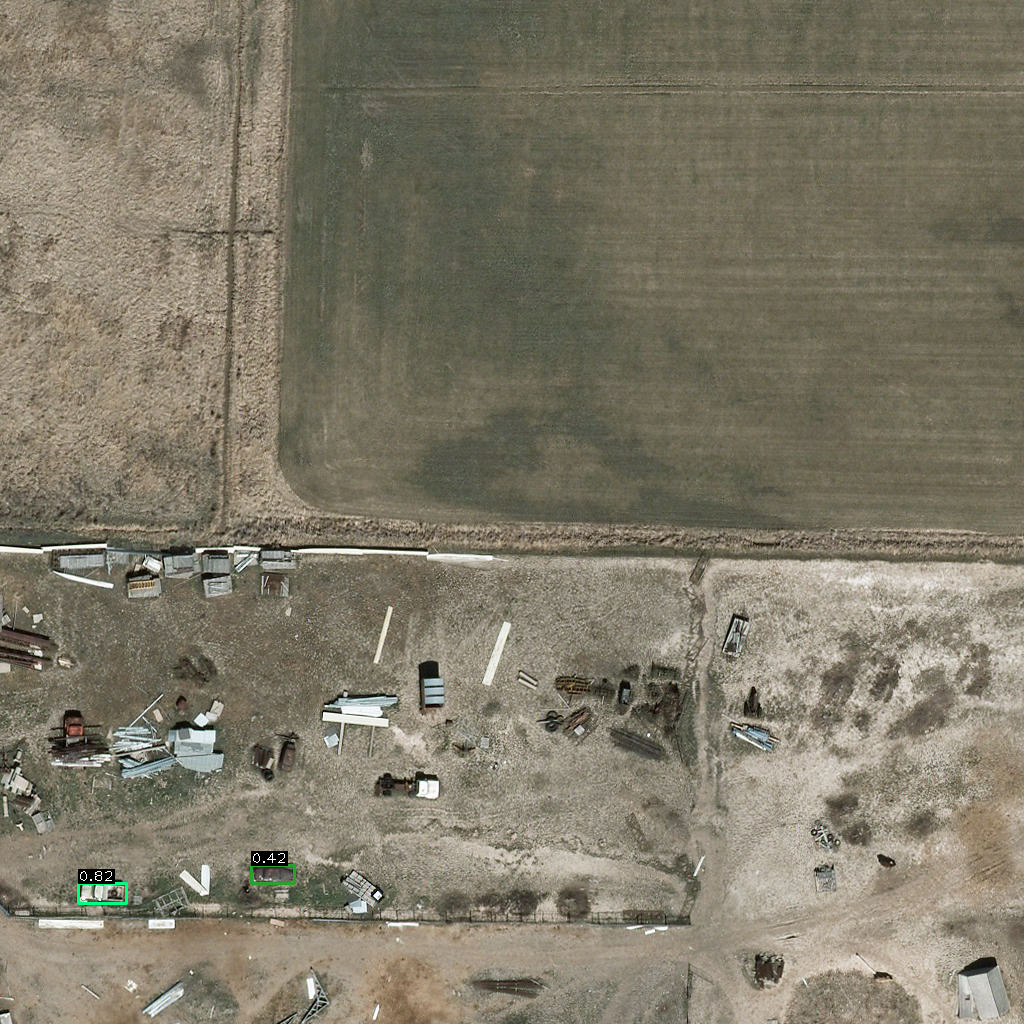
\includegraphics[trim={360pt 200pt 540pt 715pt},clip,width=\linewidth]{images/015Results/01abb_vs_obb/comp_images/abb/212.png}
    %Camping Car
    & 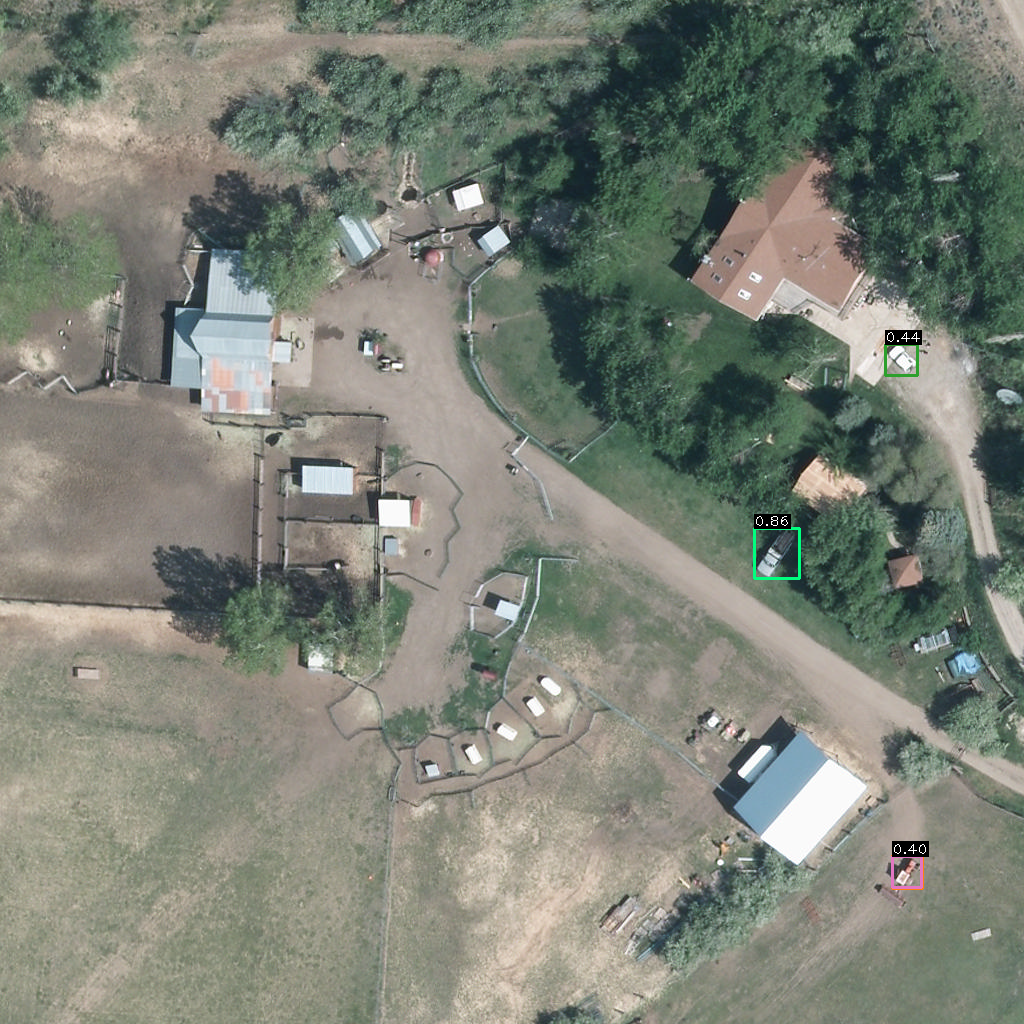
\includegraphics[trim={730pt 220pt 200pt 720pt},clip,width=\linewidth]{images/015Results/01abb_vs_obb/comp_images/abb/523.png}
    %Tractor
    & 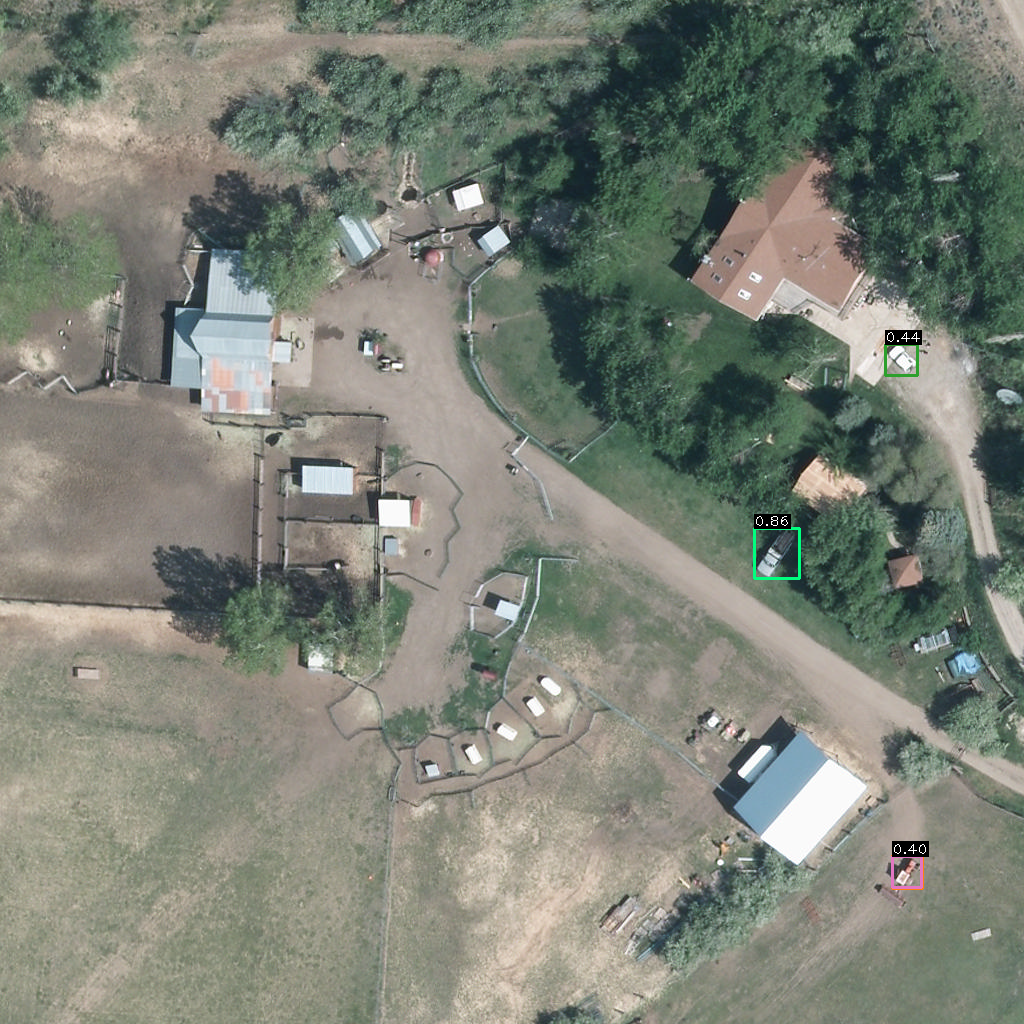
\includegraphics[trim={850pt 110pt 80pt 830pt},clip,width=\linewidth]{images/015Results/01abb_vs_obb/comp_images/abb/523.png}
    %Plane
    &  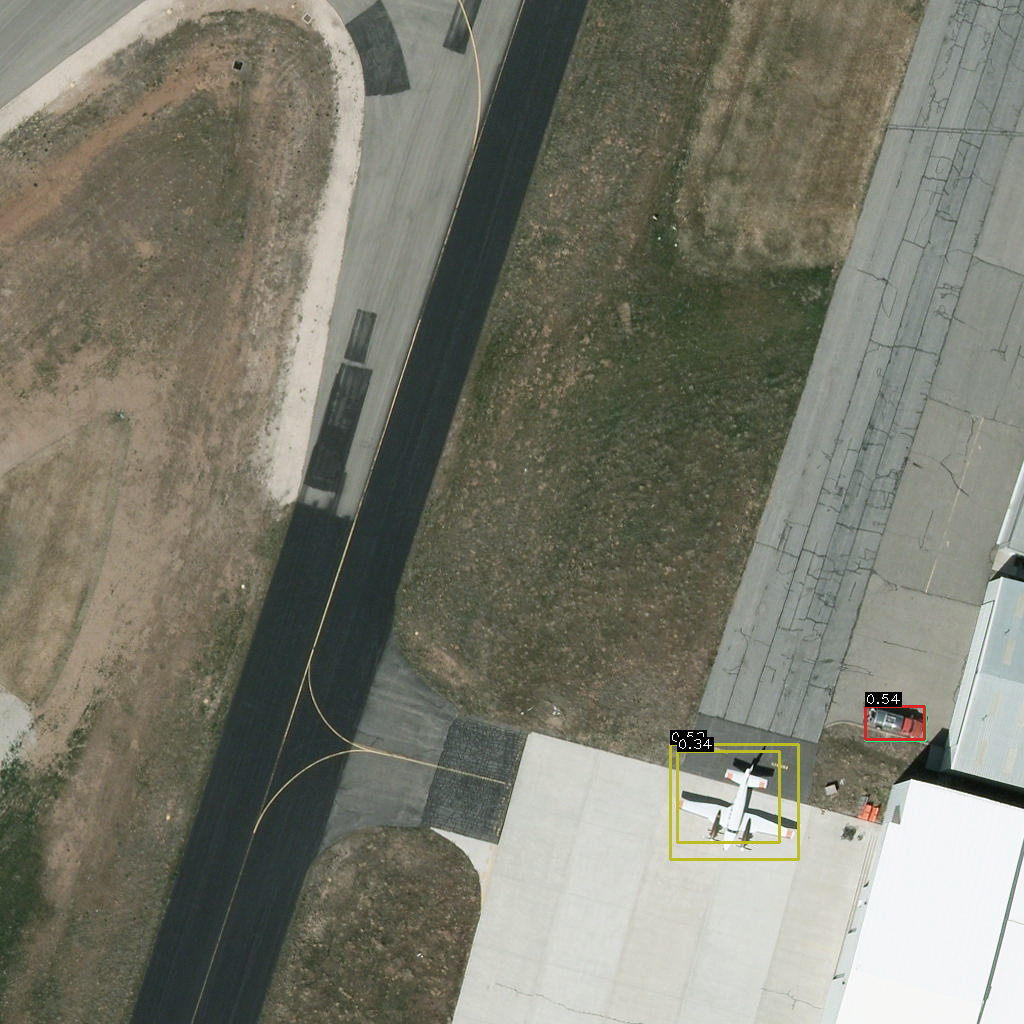
\includegraphics[trim={650pt 120pt 170pt 720pt},clip,width=\linewidth]{images/015Results/01abb_vs_obb/comp_images/abb/487.png}
    %Ship
    & 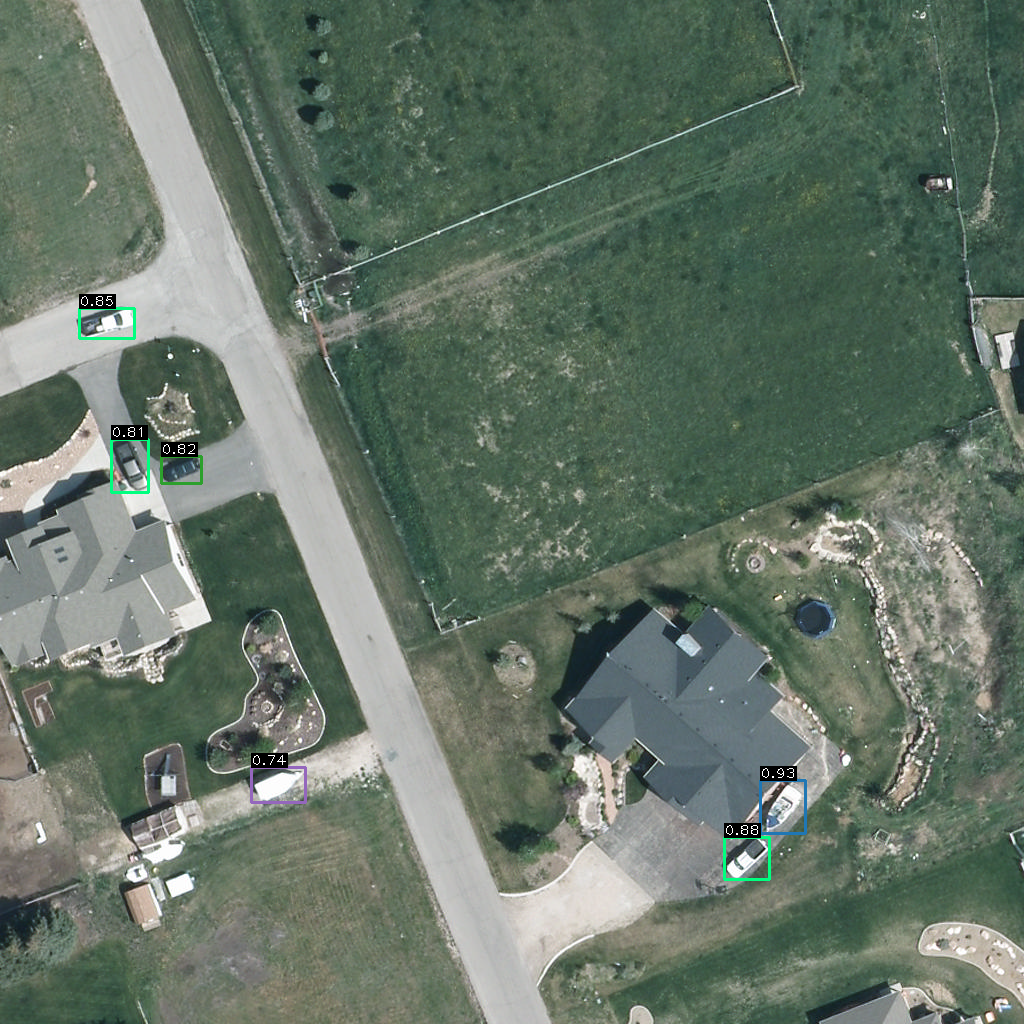
\includegraphics[trim={230pt 200pt 680pt 725pt},clip,width=\linewidth]{images/015Results/01abb_vs_obb/comp_images/abb/509.png}
    %vehicle
    & 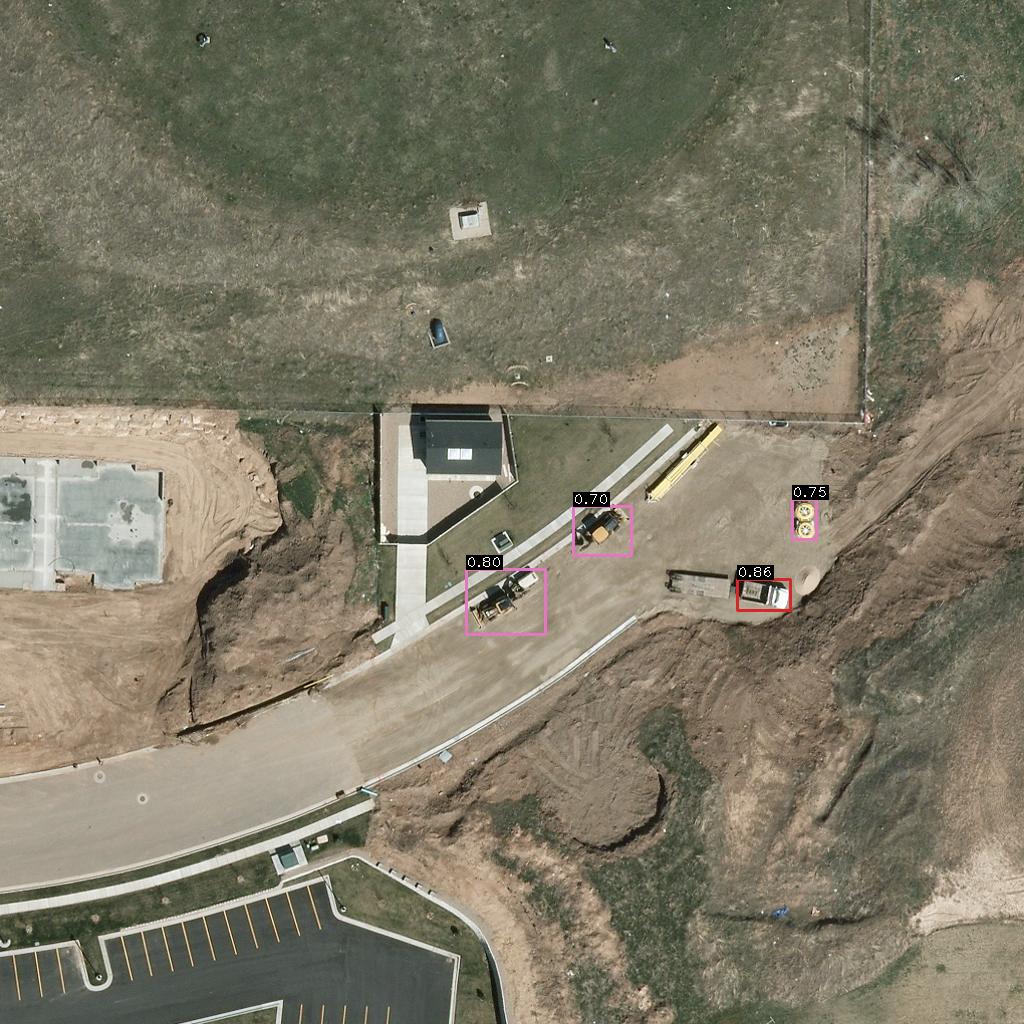
\includegraphics[trim={440pt 360pt 460pt 555pt},clip,width=\linewidth]{images/015Results/01abb_vs_obb/comp_images/abb/427.png}
    %Pick Up
    & 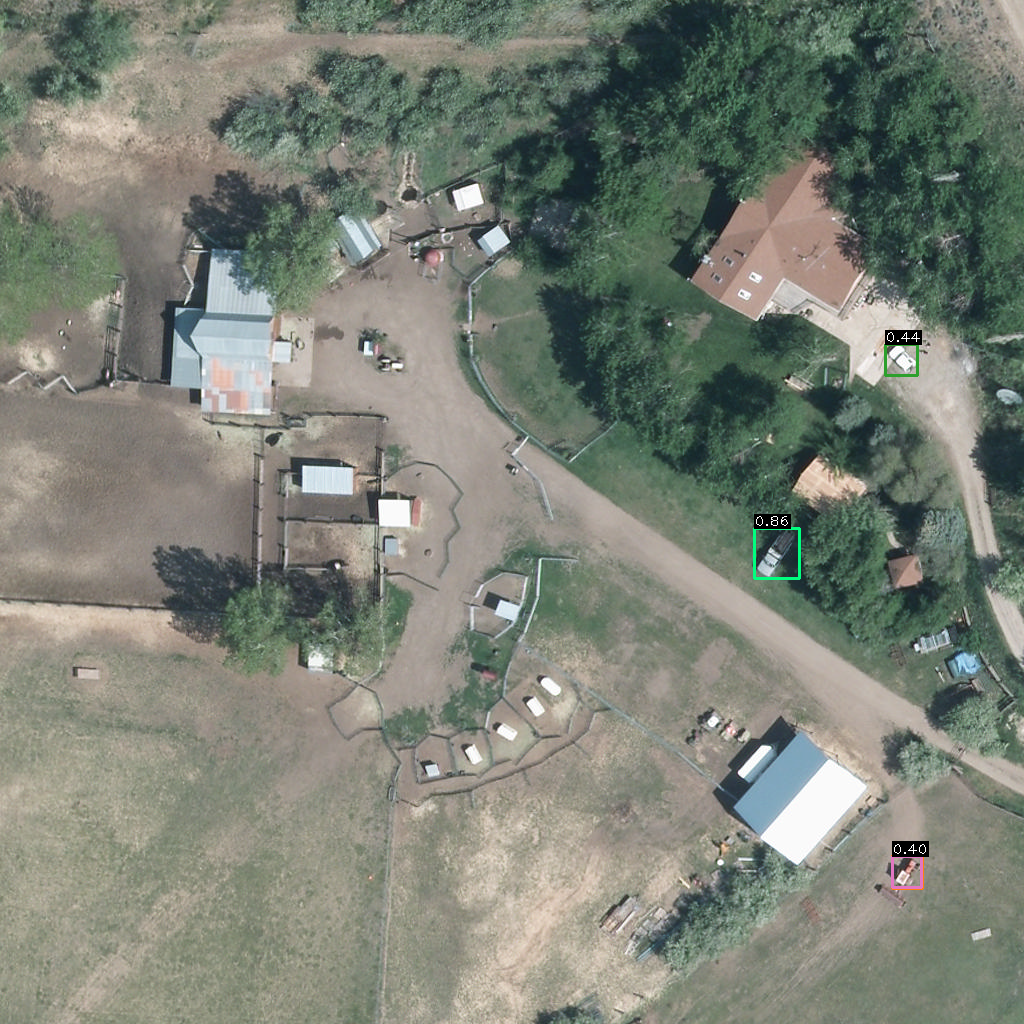
\includegraphics[trim={740pt 420pt 180pt 510pt},clip,width=\linewidth]{images/015Results/01abb_vs_obb/comp_images/abb/523.png}
    %Van
    & 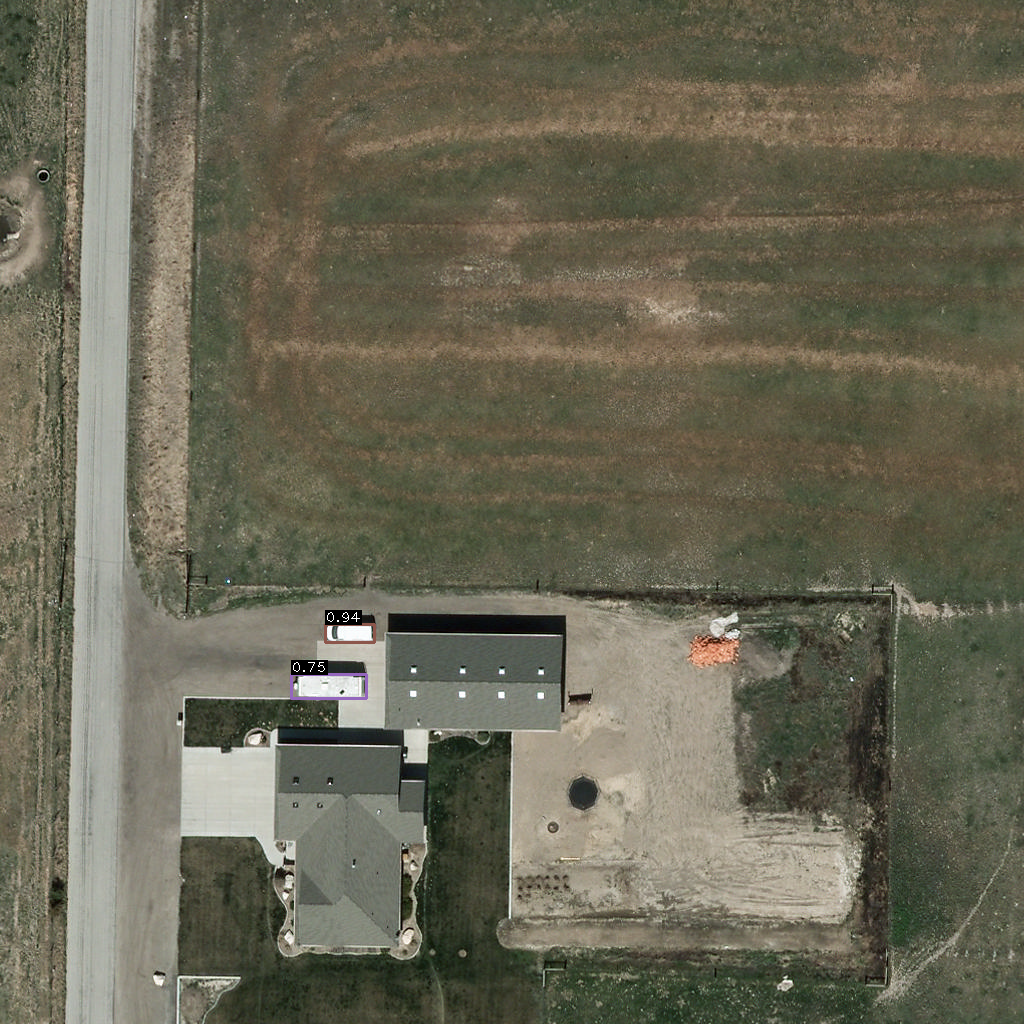
\includegraphics[trim={300pt 355pt 610pt 570pt},clip,width=\linewidth]{images/015Results/01abb_vs_obb/comp_images/abb/198.png} \\ \hline
    \rotatebox{90}{\textbf{\acrshort{obb}}} 
    %Car
    & 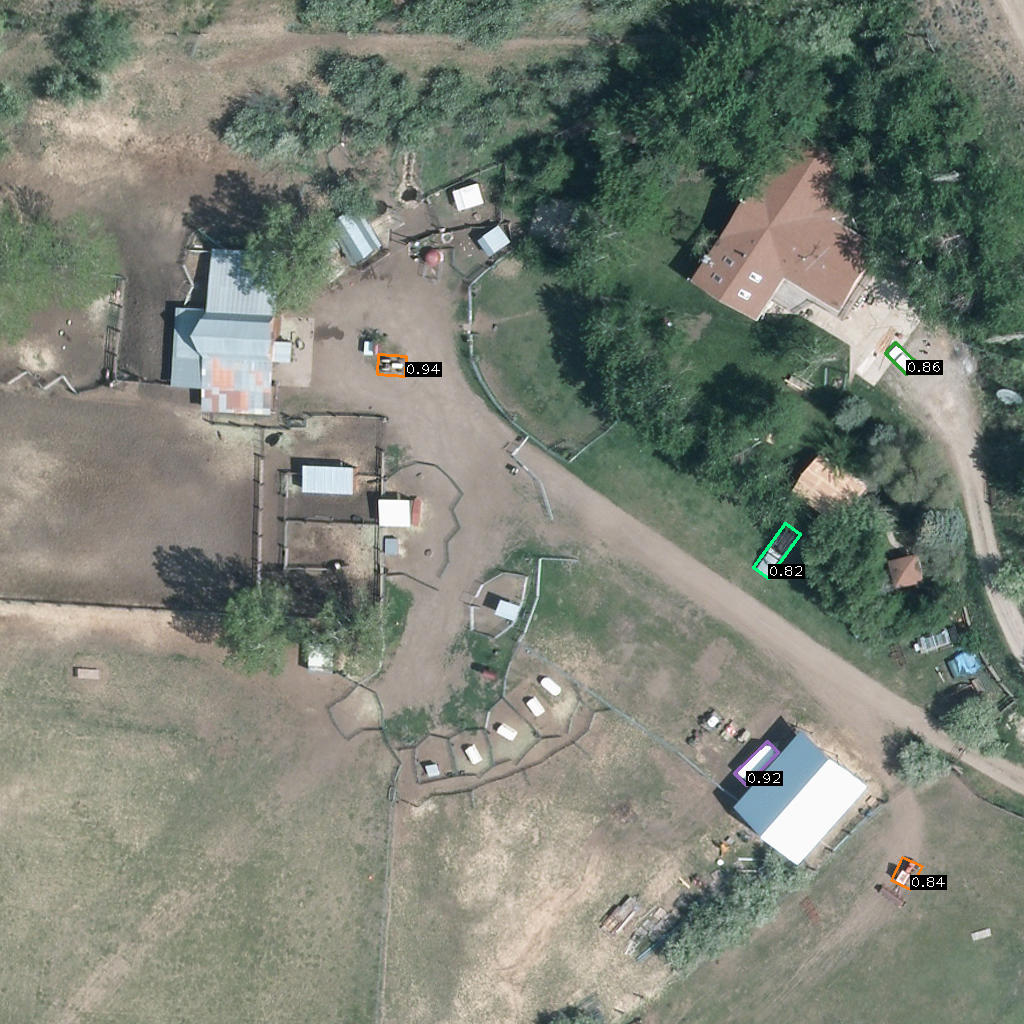
\includegraphics[trim={880pt 630pt 70pt 330pt},clip,width=\linewidth]{images/015Results/01abb_vs_obb/comp_images/obb/523.png}
    %Truck
    & 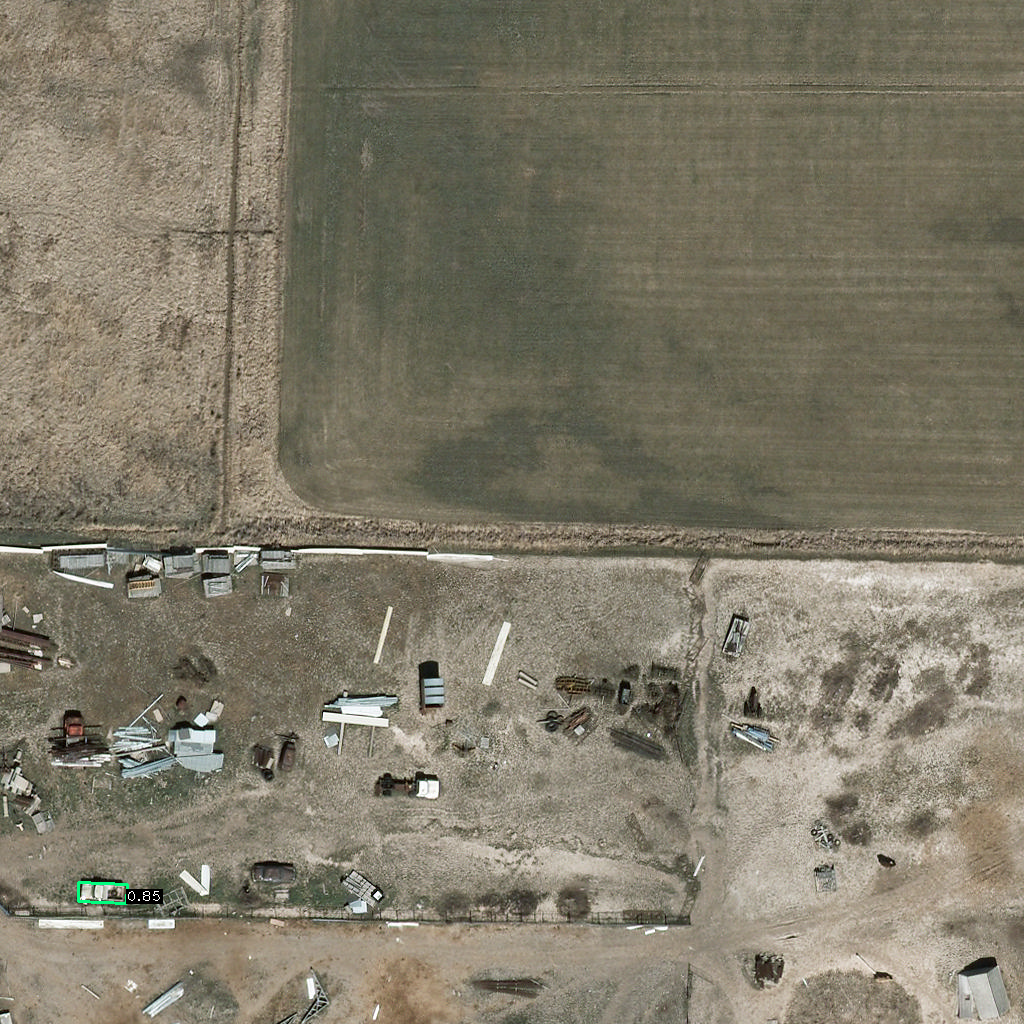
\includegraphics[trim={360pt 200pt 540pt 715pt},clip,width=\linewidth]{images/015Results/01abb_vs_obb/comp_images/obb/212.png}
    %Camping Car
    & 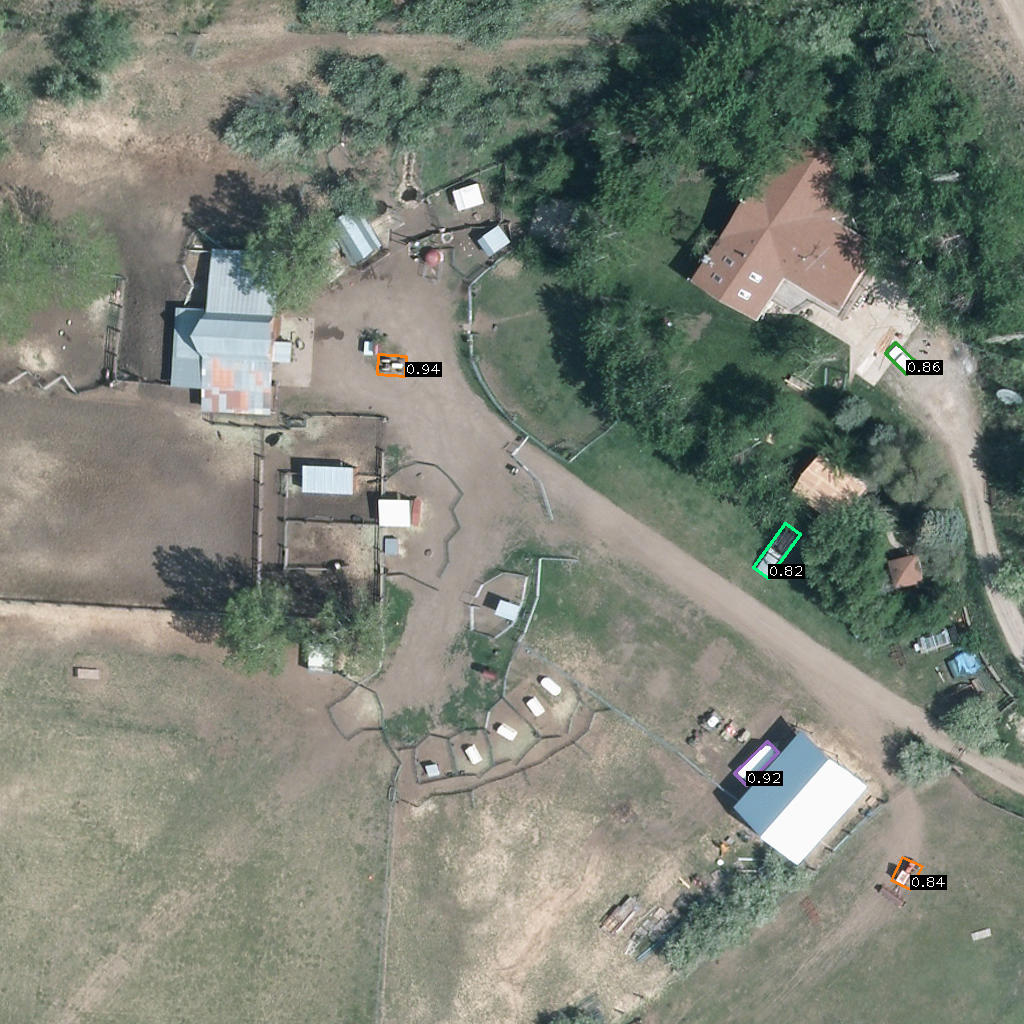
\includegraphics[trim={730pt 220pt 200pt 720pt},clip,width=\linewidth]{images/015Results/01abb_vs_obb/comp_images/obb/523.png}
    %Tractor
    & 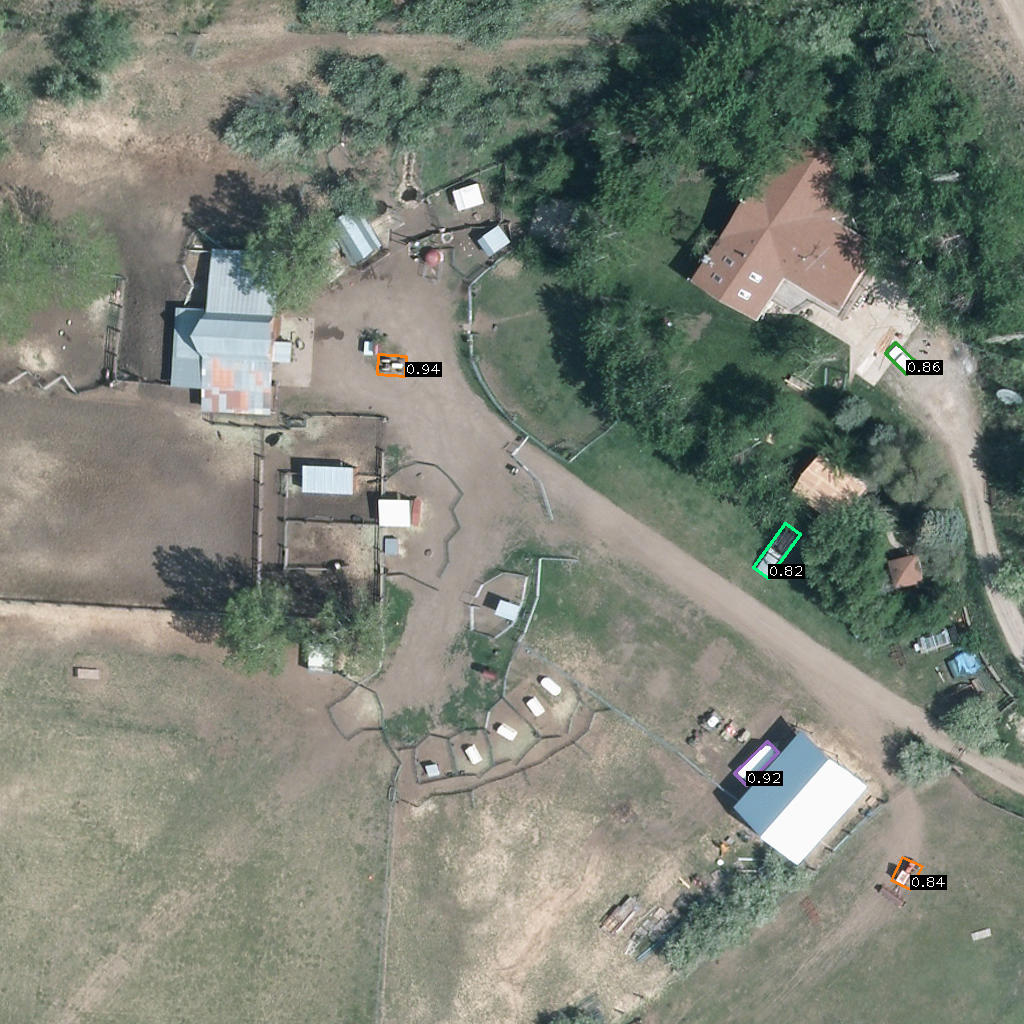
\includegraphics[trim={850pt 110pt 80pt 830pt},clip,width=\linewidth]{images/015Results/01abb_vs_obb/comp_images/obb/523.png}
    %Plane
    &  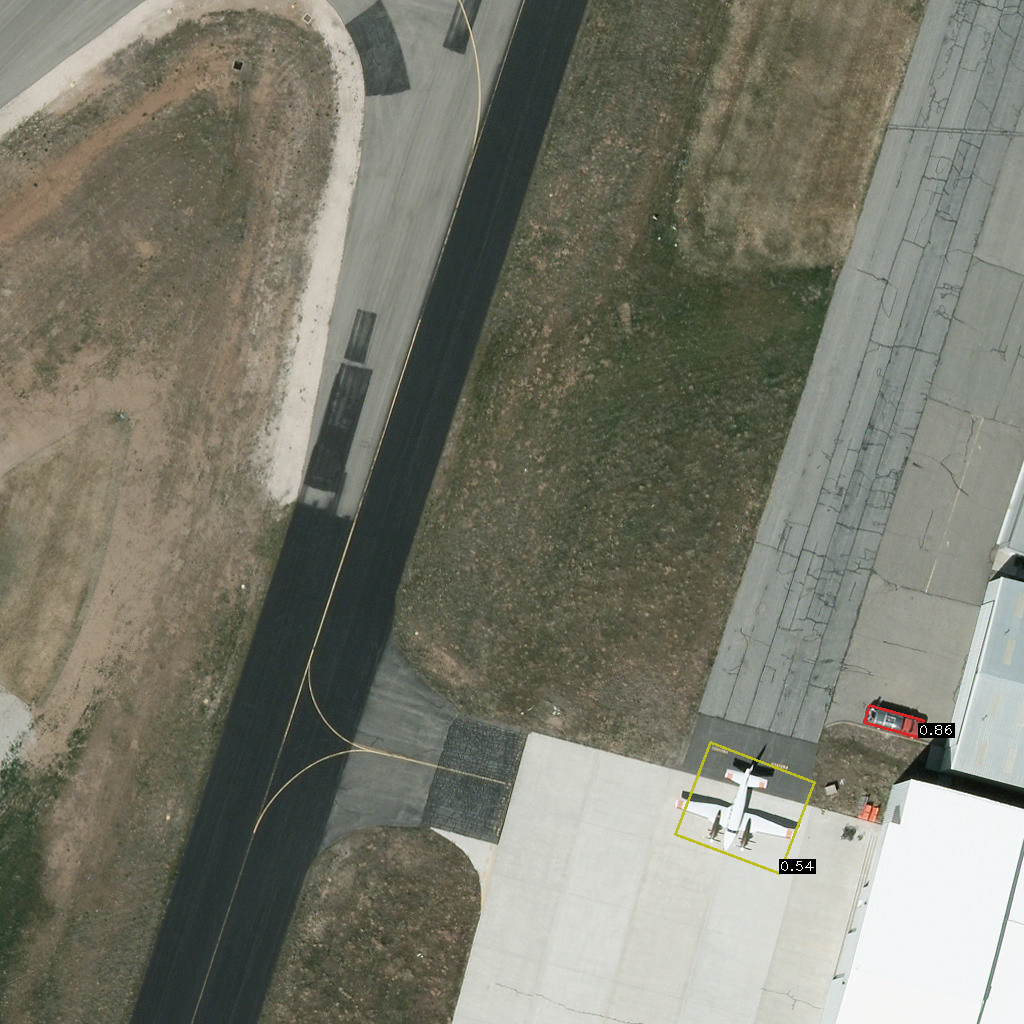
\includegraphics[trim={650pt 120pt 170pt 720pt},clip,width=\linewidth]{images/015Results/01abb_vs_obb/comp_images/obb/487.png}
    %Ship
    & 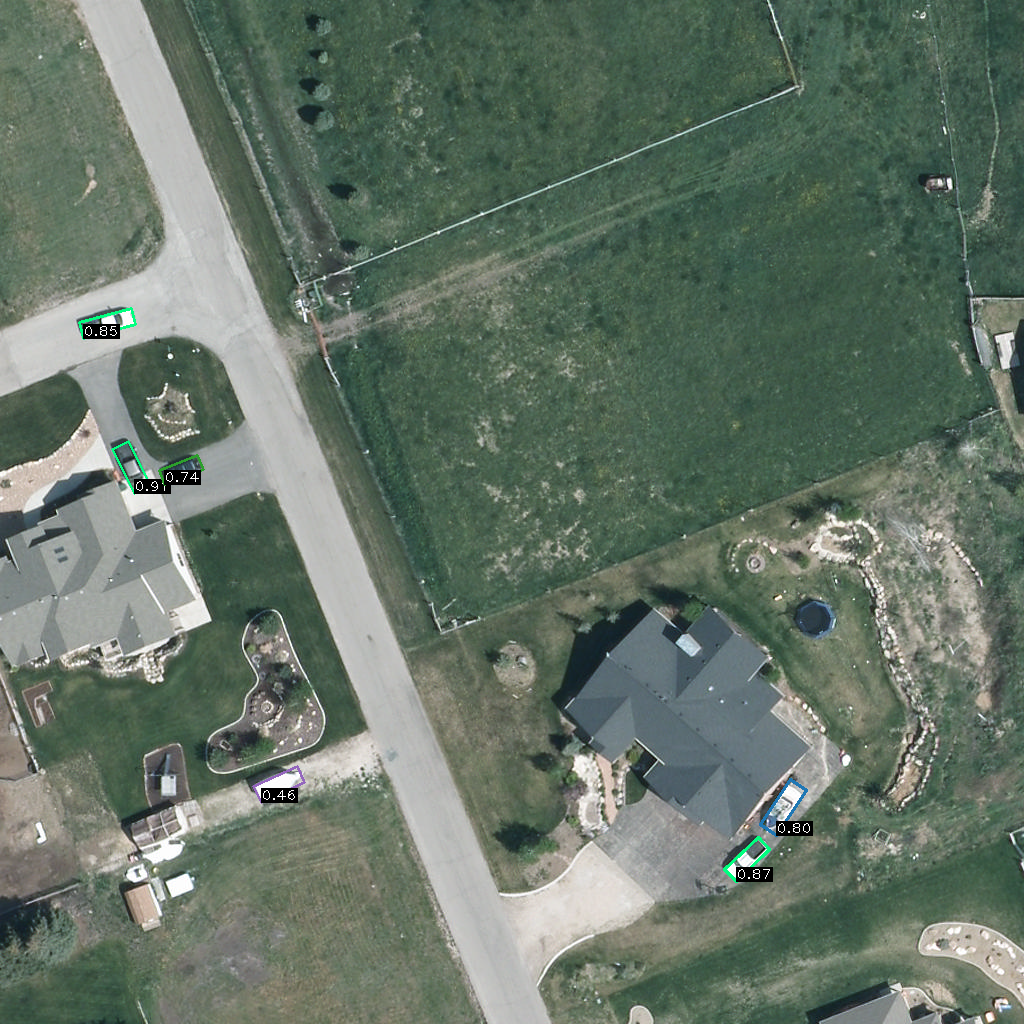
\includegraphics[trim={230pt 200pt 680pt 725pt},clip,width=\linewidth]{images/015Results/01abb_vs_obb/comp_images/obb/509.png}
    %vehicle
    & 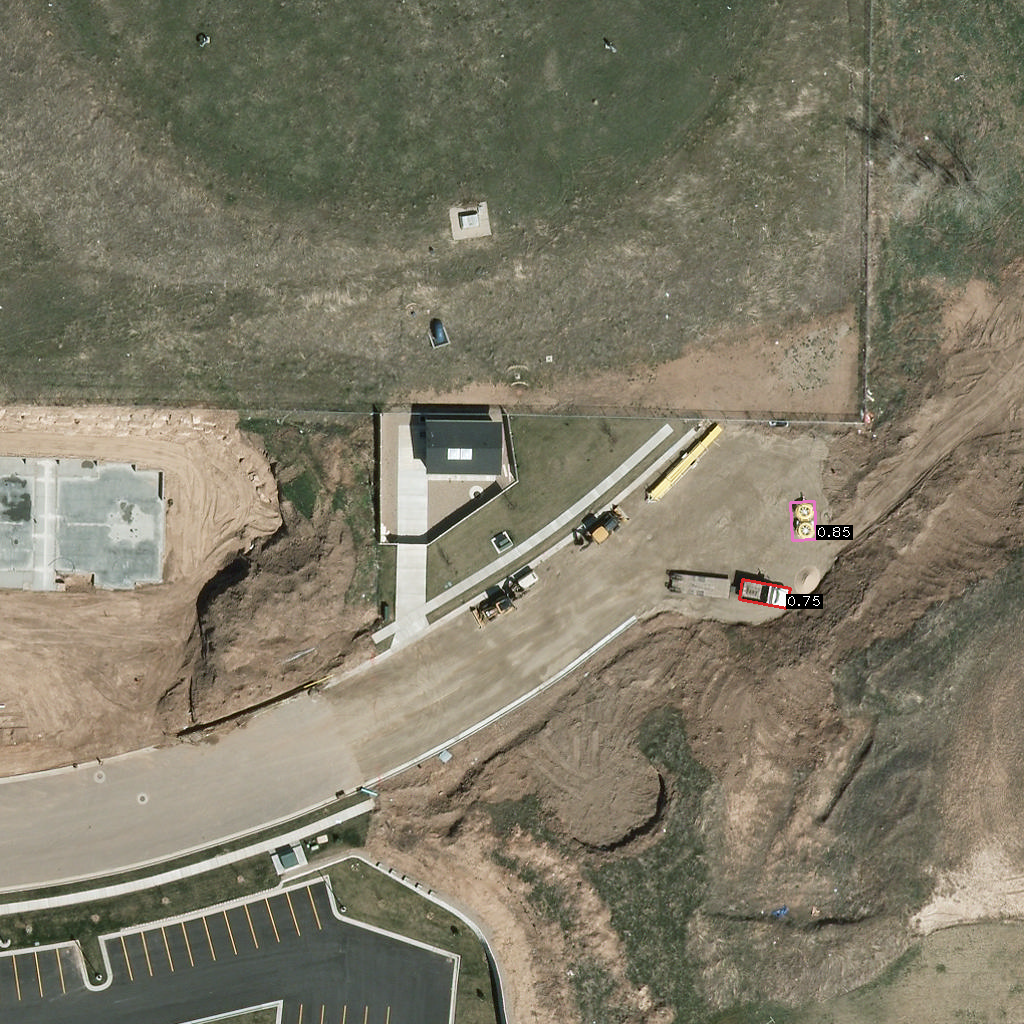
\includegraphics[trim={440pt 360pt 460pt 555pt},clip,width=\linewidth]{images/015Results/01abb_vs_obb/comp_images/obb/427.png}
    %Pick Up
    & 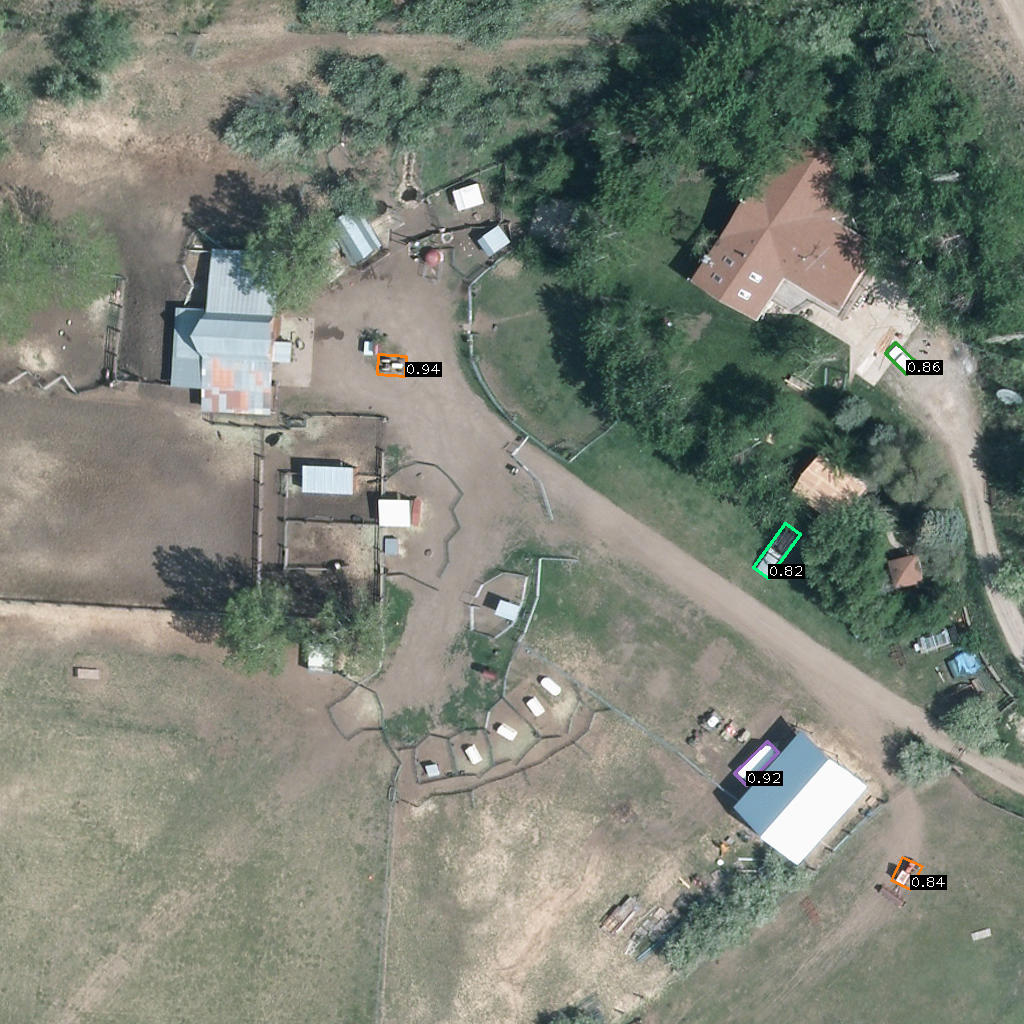
\includegraphics[trim={740pt 420pt 180pt 510pt},clip,width=\linewidth]{images/015Results/01abb_vs_obb/comp_images/obb/523.png}
    %Van
    & 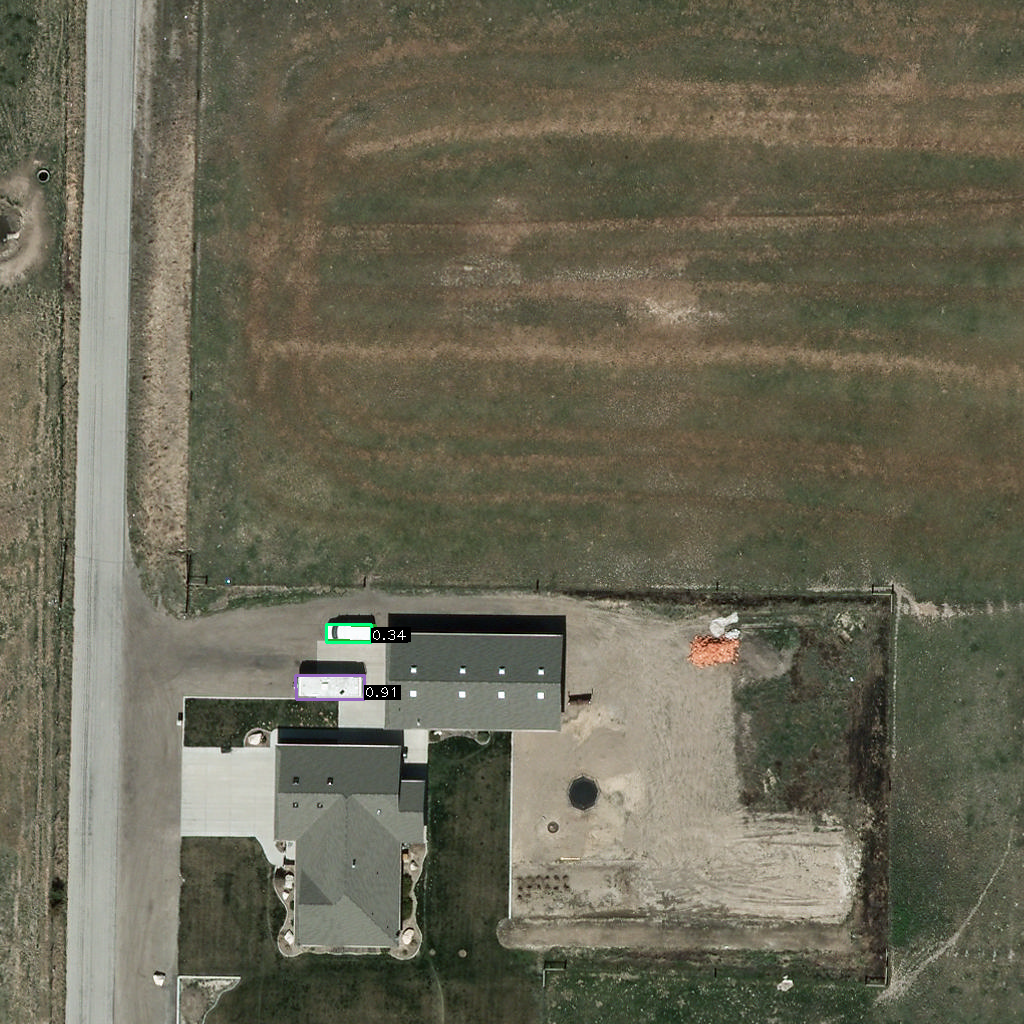
\includegraphics[trim={300pt 355pt 610pt 570pt},clip,width=\linewidth]{images/015Results/01abb_vs_obb/comp_images/obb/198.png} \\ \hline
     \rotatebox{90}{\textbf{\acrshort{abb} in \acrshort{obb}}} 
    %Car
    & 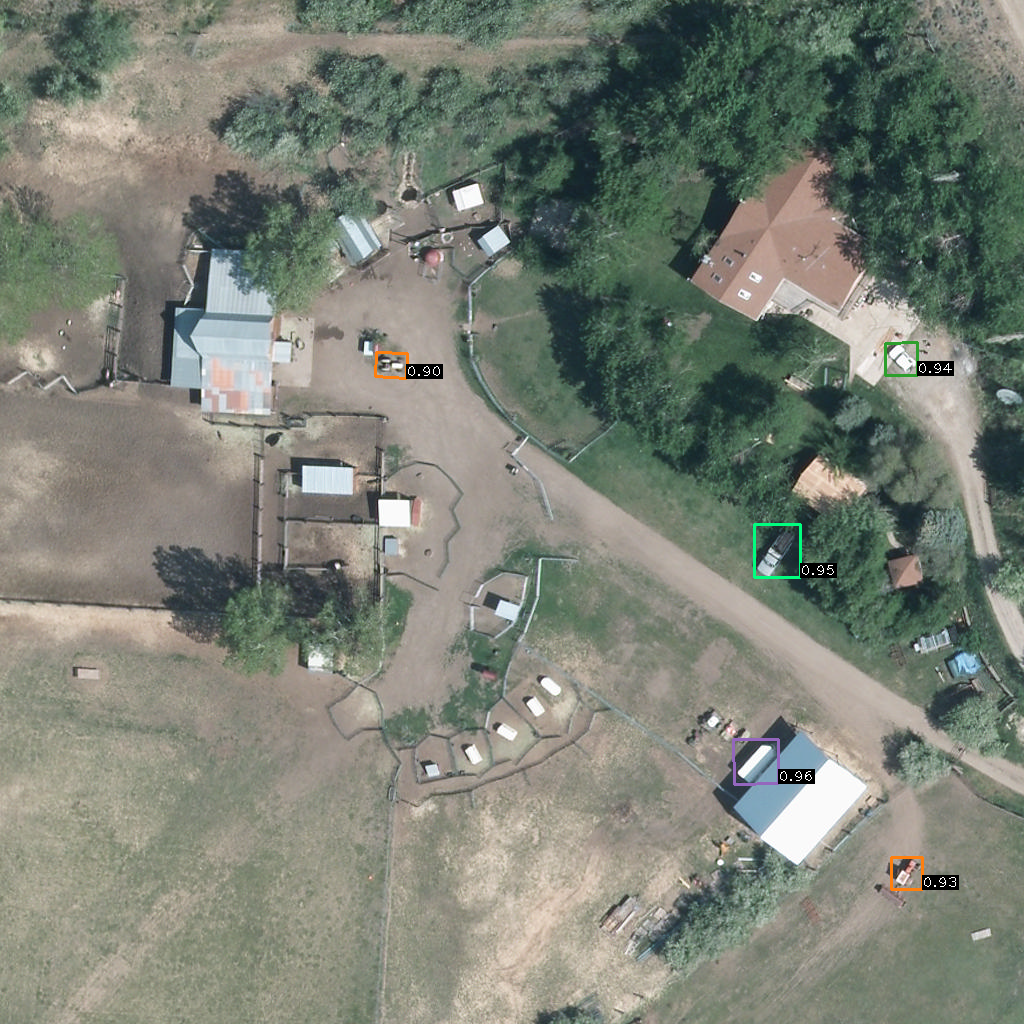
\includegraphics[trim={880pt 630pt 70pt 330pt},clip,width=\linewidth]{images/015Results/01abb_vs_obb/comp_images/aab_old/523.png}
    %Truck
    & 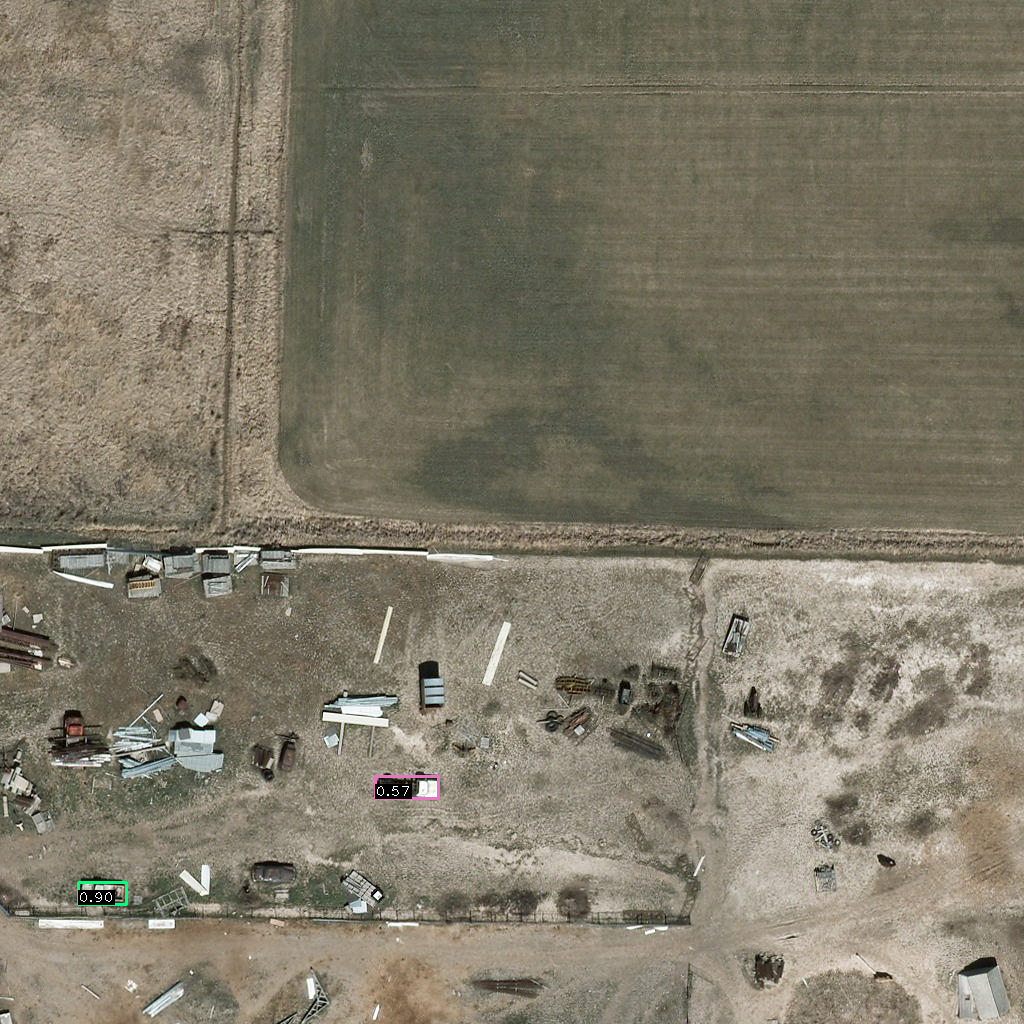
\includegraphics[trim={360pt 200pt 540pt 715pt},clip,width=\linewidth]{images/015Results/01abb_vs_obb/comp_images/aab_old/212.png}
    %Camping Car
    & 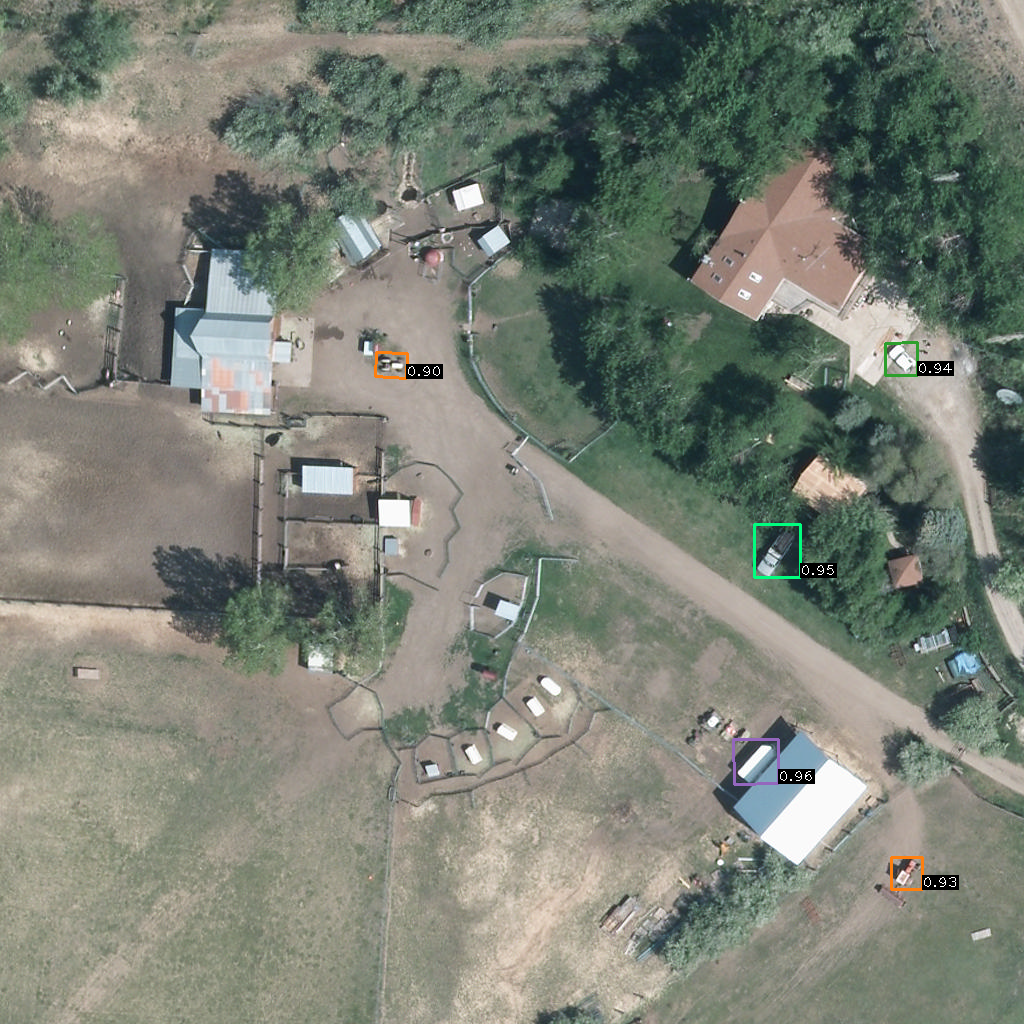
\includegraphics[trim={730pt 220pt 200pt 720pt},clip,width=\linewidth]{images/015Results/01abb_vs_obb/comp_images/aab_old/523.png}
    %Tractor
    & 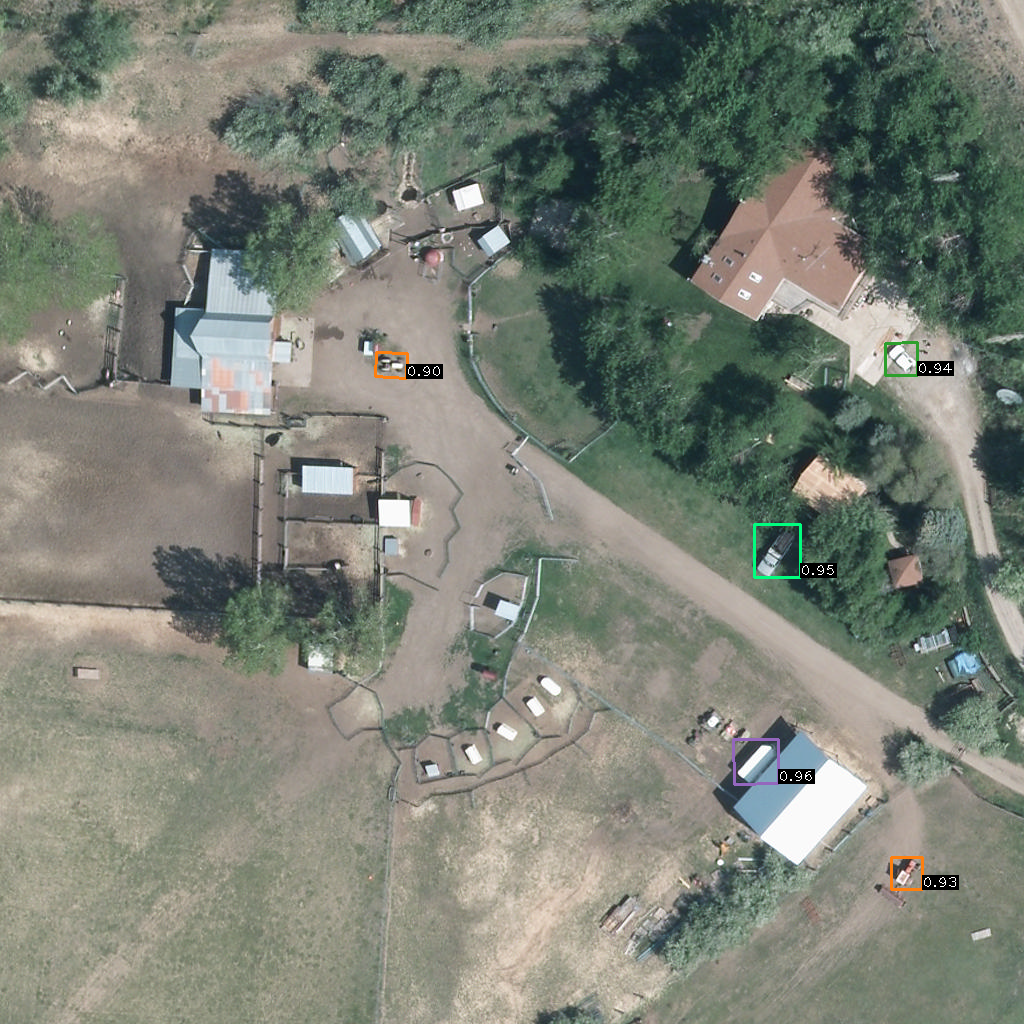
\includegraphics[trim={850pt 110pt 80pt 830pt},clip,width=\linewidth]{images/015Results/01abb_vs_obb/comp_images/aab_old/523.png}
    %Plane
    &  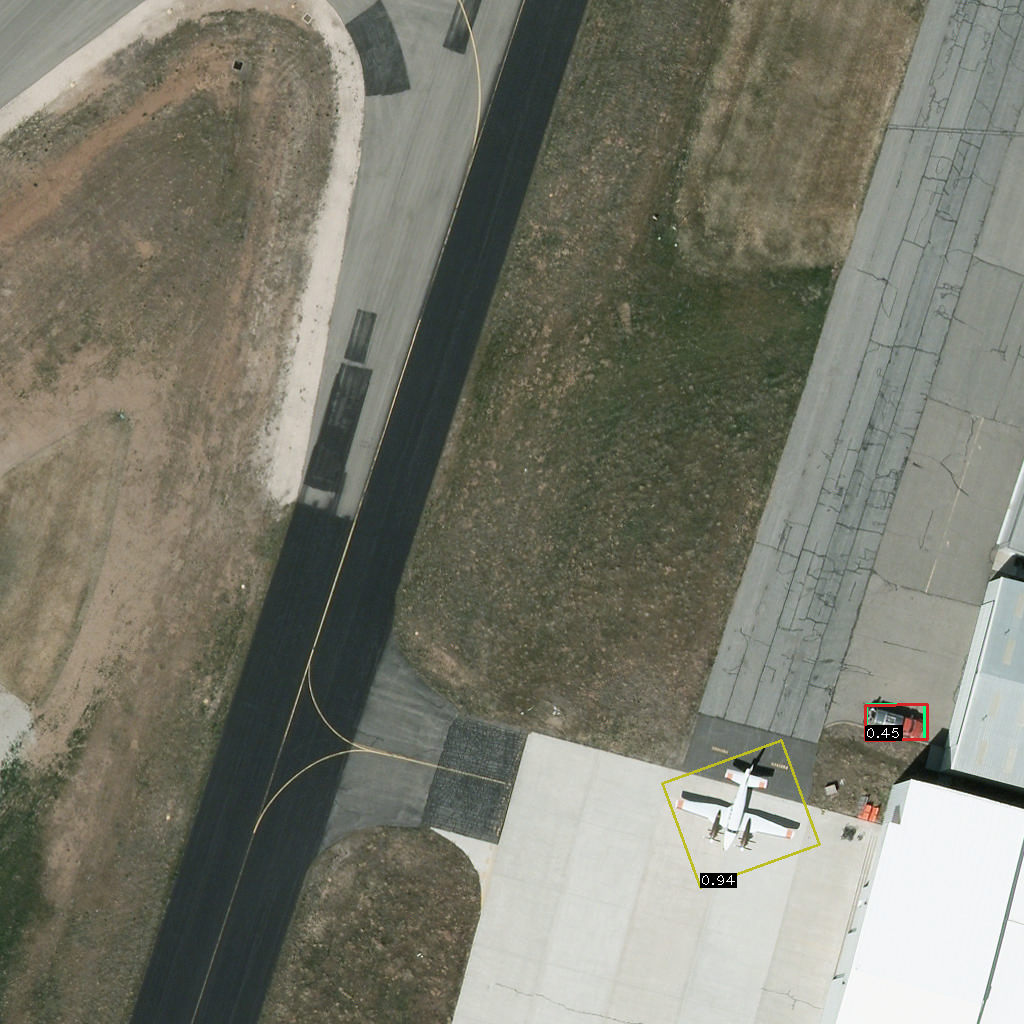
\includegraphics[trim={650pt 120pt 170pt 720pt},clip,width=\linewidth]{images/015Results/01abb_vs_obb/comp_images/aab_old/487.png}
    %Ship
    & 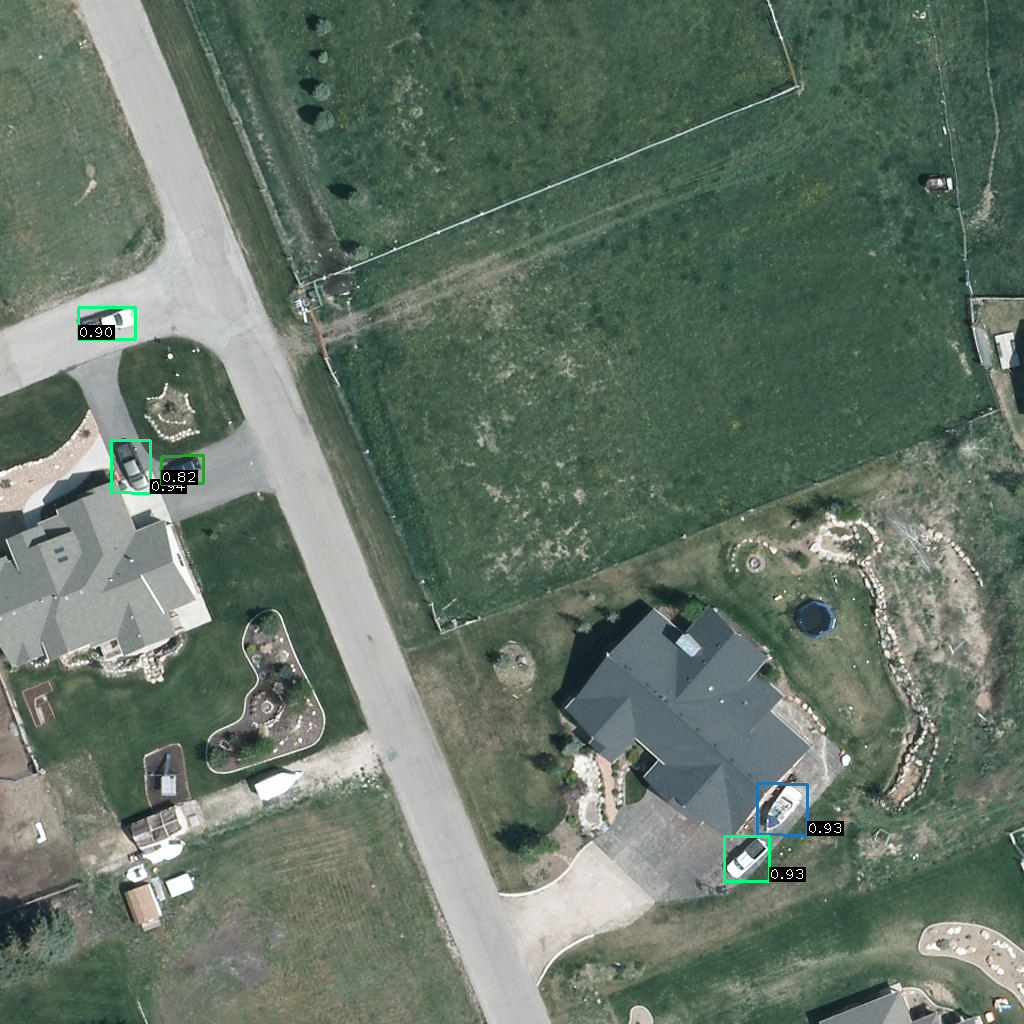
\includegraphics[trim={230pt 200pt 680pt 725pt},clip,width=\linewidth]{images/015Results/01abb_vs_obb/comp_images/aab_old/509.png}
    %vehicle
    & 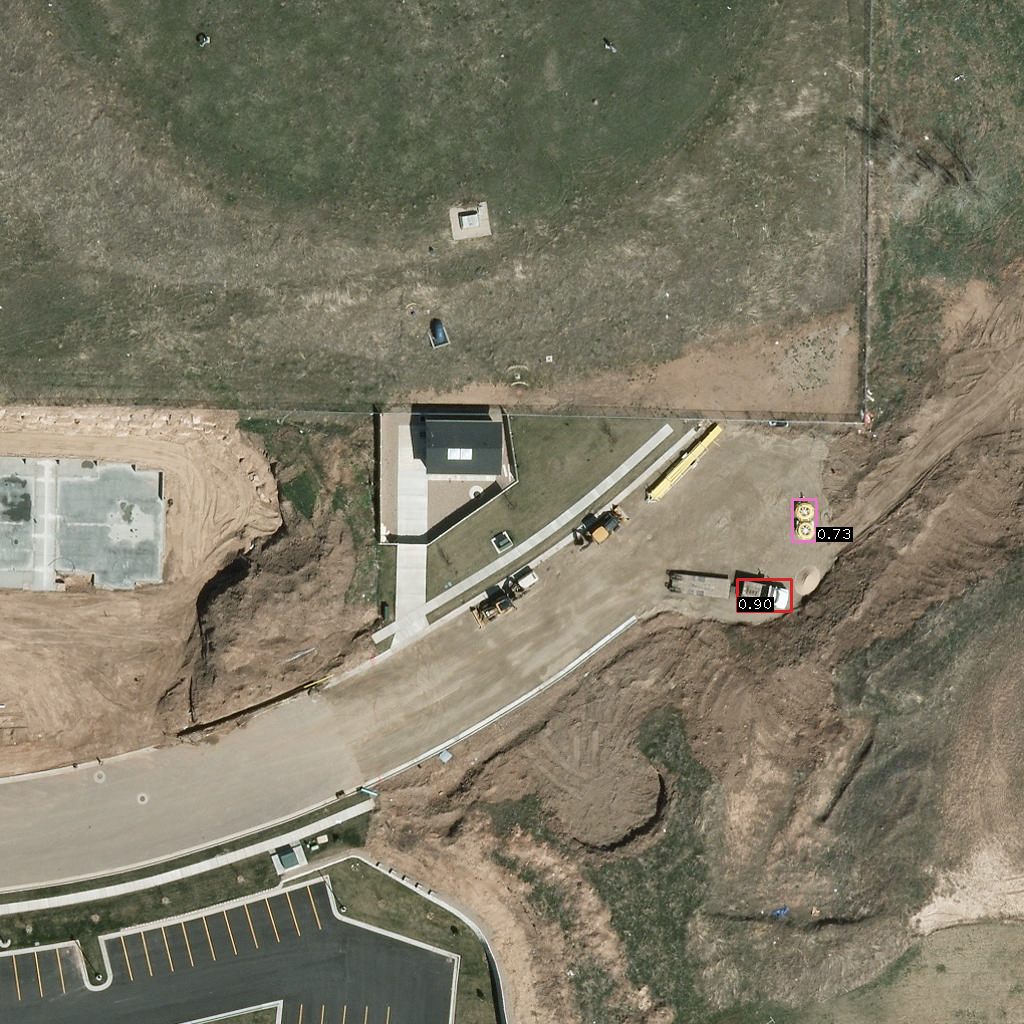
\includegraphics[trim={440pt 360pt 460pt 555pt},clip,width=\linewidth]{images/015Results/01abb_vs_obb/comp_images/aab_old/427.png}
    %Pick Up
    & 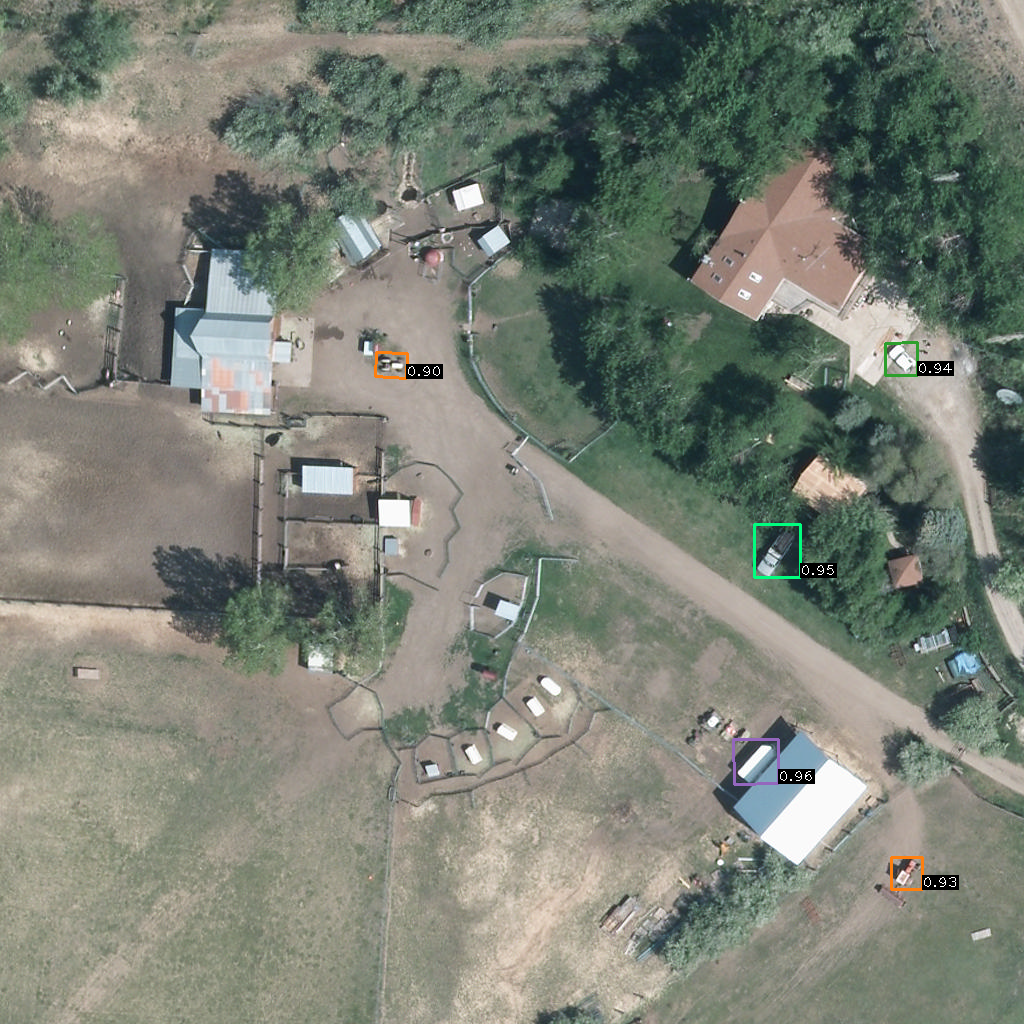
\includegraphics[trim={740pt 420pt 180pt 510pt},clip,width=\linewidth]{images/015Results/01abb_vs_obb/comp_images/aab_old/523.png}
    %Van
    & 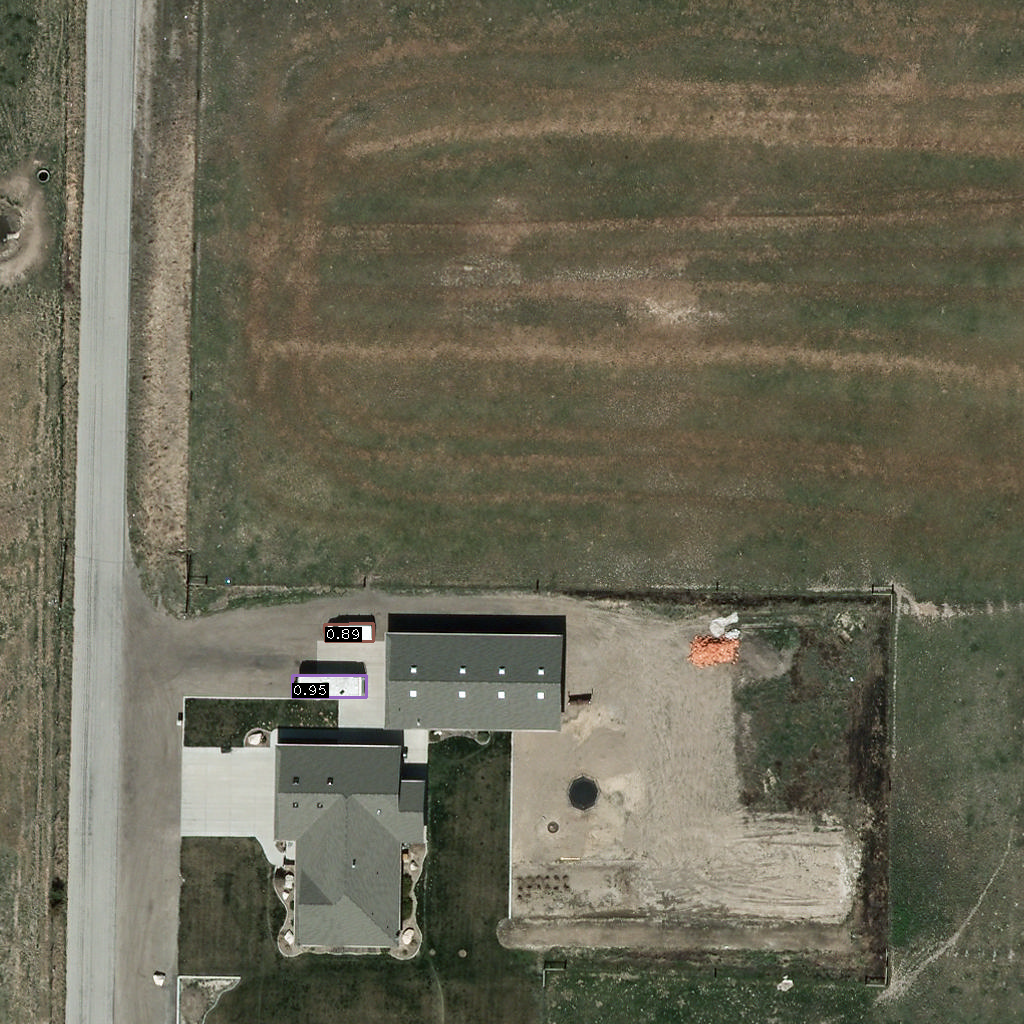
\includegraphics[trim={300pt 355pt 610pt 570pt},clip,width=\linewidth]{images/015Results/01abb_vs_obb/comp_images/aab_old/198.png} \\ \hline
\end{tabularx}
\caption[aab and obb: Examples of different classes for the object recognition performance]{Examples of different classes for the object recognition performance of different bounding box formats. The numbers displayed on the bounding boxes indicate the confidence of the model in the classification of the respective box. For Color Scheme explanation see Tab. \ref{tab:class_colors}}.
\label{fig:aab_obb_example_pics}
\end{figure}



Aufgrund der geringeren Überlappungswahrscheinlichkeit und der genaueren Objektumrandung wurde das \acrshort{obb}-Modell für die weiteren Modelle im Rahmen der Permutationstests ausgewählt.
% \begin{itemize}
%     \item Wenn man nun die \acrshort{mAP}50-95 des besten Validerungsmodells auf dem Validierungsdatensatz betrachtet (s. Fig. \ref{fig:obb_abb_map50-95:val_on_val}), sieht man das das obb Modell in jedem Fall eine bessere Performance hat als das abb Modell
%     \item Unterschied im obb Modell ist zwischen den Bounding Box Formaten vorhanden; \acrshort{abb} hat auf dem obb Modell eine höhere Leistung als die eigentlich "besseren" / angepassten \acrshort{obb} auf dem obb Modell (yolov9u)
%     \item gleiches Phänomen ist auf dem Testdatensatz zu sehen (s. Fig. \ref{fig:obb_abb_map50-95:val_on_test})
%     \item \acrshort{abb} performt besser mit dem obb modell
%     \item Konsistenz aller Modelle über die 5 Folds der Kreuzvalidierung ist gut, was eine robuste Trainierbarkeit bedeutet
%     \item obb Modell für die Permutation entschieden, da Gefahr von Überlappungen geringer und genauere Umrandung der Objekte
% \end{itemize}

\begin{figure}[htbp]
    \centering
    \includesvg[width=0.8\textwidth]{images/015Results/01abb_vs_obb/aab_obb_best_val_on_test.svg}
    \caption[Comparison of \acrshort{mAP}50-95 values for \acrshort{abb} and \acrshort{obb} (Best validation model on test dataset)]{Comparison of \acrshort{mAP}50-95 values for \acrshort{abb} and \acrshort{obb} (Best validation model on test dataset). "aab in obb" means, that \acrlong{abb} converted to obb was used in the \acrshort{YOLO}v9u model with zero rotation. The red dot is the fold, that has the best \acrshort{mAP}50-95 at the validation dataset (see fig. \ref{fig:obb_abb_map50-95:val_on_val}).(Own representation)}
    \label{fig:obb_abb_map50-95:val_on_test}
\end{figure}



% \begin{itemize}
%     \item Training Results by the mAP50-95 of all 5 Folds for every model 
%     \item Left Side (Blue): Yolov9 (without obb) and with axis aligned Bounding Boxes
%     \item Middle (Orange): Yolov9u with oriented bounding boxes
%     \item Uses Ultralytics as Backend for obb support
%     \item Right (Green): Yolov9u with axis aligned Bounding Boxes in the oriented Bounding Box format
%     \item Result -> aab performs better
%     \item \todo{Vergleichsbild eifnügen oder verweis}
%     \item This is probably due to the fact that small changes in the orientation of the bounding boxes lead to a greater deviation of the mean average precision 
%     \item Oriented Bounding boxes are smaller than the axis aligned bounding boxes -> higher inaccuracy of mAP50-95 (see next slide)
%     \item Red box at the right picture has a small deviation from the correct (blue) label
%     \item 
%     \item Konsistenz aller Modelle über die 5 Folds der Kreuzvalidierung ist gut, was eine robuste Trainierbarkeit bedeutet
% \end{itemize}
% \begin{itemize}
%     \item \todo{Bild für Vergleich der BB Area einfügen (zw. obb, aab aab old)}
%     \item Oriented Bounding Boxes has an area from around 600 to 900 pixels 
%     \item Axis aligned Bounding boxes from around 750 to 1300 px
%     \item-> higher inaccuracy of mAP50-95

%     \item For the channel permutation I used the obb model

% \end{itemize}
\FloatBarrier
%##########################################################################
%##########################################################################
%##########################################################################
%##########################################################################
%##########################################################################
%##########################################################################
%##########################################################################
%##########################################################################
%##########################################################################

\section{Permutation Experiments}
\begin{figure}[t]
    \centering
    \includesvg[width=0.9\textwidth]{images/015Results/02perm_exp/perm_exp_best_val_on_test.svg}
    \caption[Comparison of \acrshort{mAP}50-95 values for different channel permutation models (Best validation model on test dataset)]{Comparison of \acrshort{mAP}50-95 values for different channel permutation models (Best validation model on test dataset). The red dot is the fold, that has the best \acrshort{mAP}50-95 at the validation dataset (see fig. \ref{fig:perm_exp_map50-95:val_on_val}). (Own representation)}
    \label{fig:perm_exp_map50-95:val_on_test}
\end{figure}

\begin{figure}[b]
    \centering
    \includesvg[width=0.9\textwidth]{images/015Results/02perm_exp/perm_exp_best_val_on_val.svg}
    \caption[Comparison of \acrshort{mAP}50-95 values for different channel permutation models (Best validation model on validation dataset)]{Comparison of \acrshort{mAP}50-95 values for different channel permutation models (Best validation model on validation dataset).(Own representation)}
    \label{fig:perm_exp_map50-95:val_on_val}
\end{figure}
Im Folgenden werden zunächst die allgemeinen Ergebnisse der Modelle hinsichtlich der Detektionsleistung beschrieben und mit den in Abbildung \ref{fig:perm_exp_map50-95:val_on_test} dargestellten \acrshort{mAP}50--95-Werten verglichen. Anschließend erfolgt eine detaillierte Analyse der Klassenerkennungsleistung anhand der Differenzmatrizen.  

Abbildung \ref{fig:perm_exp_map50-95:val_on_test} verdeutlicht, dass das RGIR-Modell die beste \acrshort{mAP}50--95-Performance auf dem Testfold erreicht, gefolgt von den Modellen RIRB und RGB. Auffällig sind dabei die vergleichsweise hohen Unterschiede zwischen den Quantilen, was auf eine stärkere Streuung der Ergebnisse hindeutet. Das RGBIR-Modell liegt im Ranking an vierter Stelle, während das IRGB-Modell deutlich schwächer abschneidet als die zuvor genannten Modelle, jedoch immer noch bessere Ergebnisse erzielt als die beiden Modelle, die einen NDVI-Kanal beinhalten. Letztere zeigen insgesamt die schwächste Performance, was auf eine eingeschränkte Nützlichkeit des NDVI-Kanals für diese Aufgabe hindeutet. \todo{ist auch eigentlihc analyse} 

Vergleicht man die Ergebnisse mit denen des Validierungsbeispiels (vgl. Abbildung \ref{fig:perm_exp_map50-95:val_on_val}), so zeigen sich insgesamt größere Schwankungen zwischen den Quantilen. Während beim Validierungsdatensatz die Ergebnisse der meisten Modelle eng beieinanderliegen und sich lediglich die NDVI-basierten Modelle klar absetzen, weisen die Resultate auf dem Testdatensatz eine breitere Spannweite auf. Insbesondere RGIR zeigt hier die größte Quantilspanne und erreicht im Vergleich zu den fünf Hauptmodellen die schwächste Robustheit.  

Ein detaillierterer Blick auf die Klassenerkennungsleistung wird in den Differenzmatrizen (vgl. Abbildung \ref{fig:perm_exp_diffM_all}) deutlich. Diese veranschaulichen die spezifischen Stärken und Schwächen der einzelnen Modelle im Vergleich zu RGBIR. Während einige Modelle bei bestimmten Klassen deutliche Vorteile aufweisen, zeigen sich bei anderen Klassen systematische Fehlklassifikationen. So können Unterschiede von über 20\,\% bei einzelnen Klassenbeispielen auftreten, die die Gesamtbewertung einzelner Modelle maßgeblich beeinflussen.  

Tabelle \ref{tab:best_map_fold_perm_exp} fasst die Folds pro höchsten \acrshort{mAP} Wert und Modell zusammen. Während jeder Fold jeweils ein- bis zweimal  als bestes Validierungsmodell auf dem Validierungsdatensatz abschnitt, konnten nur Fold 2 und Fold 3 die Spitzenposition des besten Validierungsmodell auf dem Testdatensatz erreichen. Dies deutet darauf hin, dass die Generalisierungsfähigkeit der Modelle stark variieren kann und insbesondere die Übertragbarkeit vom Validierungs- auf den Testdatensatz nicht in allen Fällen konsistent ist.  \todo{ist eigenltihc analyse}

% \begin{itemize}
%     \item erst allgemeine Beschreibung mit map vergleichen und dann tiefer in die Details der KLassenerkennungsleistung der einzelnen Modelle mit Differenzmatrixen
%     \item Abb. \ref{fig:perm_exp_map50-95:val_on_test} zeigt, dass RGIR Modell hat die beste \acrshort{mAP}50-95 Leistung auf dem Testfold: dann rirb and RGB Modell
%     \item relativ hohe Differenzen zwischen den Quantilen
%     \item RGBIR ist an vierter Stelle,
%     \item IRGB ist deutlich schlechter als die anderen Modelle aber besser als die Modelle mit NDVI
%     \item Modelle mit NDVI Kanal schneiden deutlich schlechter ab
%     \item Insgesamt stärkere Schwankungen zwischen den Quantilen als beim Validierungsmodellbeispiel (s. Fig. \ref{fig:perm_exp_map50-95:val_on_val}.). Hier sind die Quantiler der ersten Modelle näher beieinander, nur die beiden ndvi modelle sind deutlich schlechter; rgir hat die größe Quantils spannweite und ist am schlechtesten von den 5 Hauptmodellen
%     \item Tab. \ref{tab:best_map_fold_perm_exp} zeigt, dass beim besten Validerungsmodell auf dem Validierungsdatensatz alle Folds ein oder zweimal am besten abgeschnitten haben; bei besten Validerungsmodell auf dem Testdatensatz nur Fold 2 und 3
% \end{itemize}




\begin{table}[h!]
\centering

\begin{tabular}{lcc}
\hline
\textbf{Model} & \textbf{Best mAP Fold (Validation)} & \textbf{Best mAP Fold (Test)} \\ \hline
RGBIR    & 0 & 2 \\
RGB      & 0 & 2 \\
IRGB     & 1 & 3 \\
RIRB     & 4 & 2 \\
RGIR     & 3 & 3 \\
GBNDVI   & 1 & 2 \\
RGBNDVI  & 4 & 2 \\ \hline
\end{tabular}
\caption{Best mAP folds for validation and test sets}
\label{tab:best_map_fold_perm_exp}
\end{table}



% \todo{wirklich clearpage nutzen?}
% %\clearpage

\FloatBarrier
\subsection{Comparison with Confusion Matrices}
\label{subsec:permexp_comp_confusion_matric}
\todo{erklären warum die letzte spalte nie beschrieben wird?}
\todo{irgendow kurz erklären wie eine differenzmatrix erzeugt wird? }


\begin{figure}[htbp]
    \centering
    \includesvg[width=0.9\textwidth]{images/015Results/02perm_exp/confusion_matrices/rgbir_F2.svg}
    \caption[Confusion Matrix for RGBIR Modell (Fold 2)]{Confusion Matrix for RGBIR Modell (Fold 2). All values falling within the interval [–0.05, 0.05] are excluded from the matrix. (Own representation)}
    \label{fig:perm_exp_confM_rgbir_f2}
\end{figure}

Die in Abbildung~\ref{fig:perm_exp_confM_rgbir_f2} dargestellte Confusion Matrix für das RGBIR-Modell (Fold~2) zeigt eine sehr starke Leistung. Insbesondere bei der Klasse \textit{plane} erreicht das Modell eine perfekte Erkennungsrate von 100~\%. Auch die Klassen \textit{car}, \textit{ship}, \textit{tractor} weisen eine hervorragende Performance von über 80~\% auf. Gute Ergebnisse im Bereich von 60–80~\% werden für die Klassen \textit{truck}, \textit{camping car}, \textit{van} und \textit{pick up} erzielt. Die generische Klasse \textit{vehicle} zeigt mit über 52~\% eine akzeptable Erkennungsrate. Problematisch ist hingegen, dass die Klasse \textit{Vehicle} häufig als \textit{Background} fehlklassifiziert wird (über 40~\%). Zusätzlich tritt eine erhöhte Fehlklassifikationsrate bei \textit{camping car} (28~\%) und \textit{truck} (16~\%) auf, während die restlichen Klassen zwischen 8–12~\% liegen. Aufgrund dieser starken Gesamtleistung dient das RGBIR-Modell (Fold~2) als Basis für die Differenzmatrizen. Ausschlaggebend ist auch, dass in diesem Permutationsdurchlauf alle verfügbaren Bänder unverändert in Rohform enthalten sind.

Zur Interpretation der Differenzmatrizen gilt: Rot markiert eine bessere Performance des RGBIR (F2) Modells, Blau eine bessere Leistung des Vergleichsmodells. Je stärker die Farbintensität, desto größer der Unterschied. Die Unterschiede werden in vier Kategorien eingeteilt: gering (0–5~\%), moderat (5–10~\%), hoch (10–20~\%) und sehr hoch (>20~\%) (Tabelle~\ref{tab:diff_cat}). Die Vergleichsreihenfolge startet mit dem schwächsten Modell und arbeitet sich bis zum besten Modell gemäß den Ergebnissen aus Abbildung~\ref{fig:perm_exp_map50-95:val_on_test} vor.

\begin{table}[h]
\centering
\begin{tabular}{c c}
\hline
\textbf{Difference (in \% from reference)} & \textbf{Category} \\ \hline
0 -- 5 \%   & low \\ 
5 -- 10 \%  & moderate \\ 
10 -- 20 \% & high \\ 
> 20 \%     & very high \\ \hline
\end{tabular}
\caption{Classification of differences relative to the reference}
\label{tab:diff_cat}
\end{table}

\begin{figure}[htbp]
    \centering
    % Erste Spalte
    \begin{subfigure}{0.48\textwidth}
        \centering
        \includesvg[width=\linewidth]{images/015Results/02perm_exp/confusion_matrices/Difference_Matrices/RGBIR_F2_vs_RGBNDVI_F2.svg}
        \caption{RGBNDVI (F2)}
        \label{fig:perm_exp_diffM_rgbndvi_f2}
    \end{subfigure}
    \begin{subfigure}{0.48\textwidth}
        \centering
        \includesvg[width=\linewidth]{images/015Results/02perm_exp/confusion_matrices/Difference_Matrices/RGBIR_F2_vs_GBNDVI_F2.svg}
        \caption{GBNDVI (F2)}
        \label{fig:perm_exp_diffM_gbndvi_f2}
    \end{subfigure}
    
    \begin{subfigure}{0.48\textwidth}
        \centering
        \includesvg[width=\linewidth]{images/015Results/02perm_exp/confusion_matrices/Difference_Matrices/RGBIR_F2_vs_IRGB_F3.svg}
        \caption{IRGB (F3)}
        \label{fig:perm_exp_diffM_irgb_f3}
    \end{subfigure}
    \begin{subfigure}{0.48\textwidth}
        \centering
        \includesvg[width=\linewidth]{images/015Results/02perm_exp/confusion_matrices/Difference_Matrices/RGBIR_F2_vs_RIRB_F2.svg}
        \caption{RIRB (F2)}
        \label{fig:perm_exp_diffM_RIRB_f2}
    \end{subfigure}
    
    \begin{subfigure}{0.48\textwidth}
        \centering
        \includesvg[width=\linewidth]{images/015Results/02perm_exp/confusion_matrices/Difference_Matrices/RGBIR_F2_vs_RGB_F2.svg}
        \caption{RGB (F2)}
        \label{fig:perm_exp_diffM_RGB_f2}
    \end{subfigure}
    \begin{subfigure}{0.48\textwidth}
        \centering
        \includesvg[width=\linewidth]{images/015Results/02perm_exp/confusion_matrices/Difference_Matrices/RGBIR_F2_vs_RGIR_F3.svg}
        \caption{RGIR (F3)}
        \label{fig:perm_exp_diffM_RGIR_f3}
    \end{subfigure}

    \caption[Difference Matrices compared to RGBIR (Fold 2)]{Difference Matrices for all models compared against RGBIR (Fold 2). Red indicates better performance for RGBIR, blue for the respective comparison model. All values falling within the interval [–0.05, 0.05] are excluded from the matrices.}
    \label{fig:perm_exp_diffM_all}
\end{figure}
\todo{Beschreibung Figures länger machen, mehr Analyse weniger "was sieht man"}

% \begin{figure}[b]
%     \centering
%     \includesvg[width=0.9\textwidth]{images/015Results/02perm_exp/confusion_matrices/Difference_Matrices/RGBIR_F2_vs_RGBNDVI_F2.svg}
%     \caption[Difference Matrix for RGBNDVI (Fold 2)]{Difference Matrix for RGBNDVI (Fold 2). (Own representation)}
%     \label{fig:perm_exp_diffM_rgbndvi_f2}
% \end{figure}

Abbildung~\ref{fig:perm_exp_diffM_rgbndvi_f2} verdeutlicht deutliche Unterschiede zugunsten von RGBIR. Besonders stark zeigt sich dies bei der korrekten Erkennung von \textit{ship} (24~\%), \textit{vehicle} (16~\%), \textit{plane} (12~\%) und \textit{tractor} (10~\%). Auch bei Verwechslungen zwischen \textit{car} und \textit{van} treten Unterschiede von mehr als 10~\% auf. Dagegen weist RGBNDVI weniger hohe Fehlklassifikationen auf, beispielsweise bei \textit{plane} (12~\%) und \textit{van} (23~\%), die weniger häufig fälschlich als \textit{background} erkannt werden. Insgesamt zeigt RGBIR fünf Klassen (\textit{Ship}, \textit{Tractor}, \textit{Vehicle}, \textit{Plane}), in denen es mindestens 5~\% besser abschneidet, während RGBNDVI keinen Vorteil verzeichnen kann.

% \begin{figure}[t]
%     \centering
%     \includesvg[width=0.9\textwidth]{images/015Results/02perm_exp/confusion_matrices/Difference_Matrices/RGBIR_F2_vs_GBNDVI_F2.svg}
%     \caption[Difference Matrix for GBNDVI (Fold 2)]{Difference Matrix for GBNDVI (Fold 2). (Own representation)}
%     \label{fig:perm_exp_diffM_gbndvi_f2}
% \end{figure}

In Abbildung~\ref{fig:perm_exp_diffM_gbndvi_f2} zeigt sich ein sehr hoher Unterschied bei der Klasse \textit{tractor}, wo RGBIR deutlich überlegen ist. Die Verbesserung bei \textit{ship} beträgt dagegen lediglich 8~\%. Auffällig ist, dass \textit{tractor}, \textit{ship} und \textit{van} im GBNDVI-Modell weniger häufig fälschlich als \textit{background} klassifiziert werden. Insgesamt ist RGBIR in vier Klassen (\textit{Ship}, \textit{Tractor}, \textit{Van}, \textit{Vehicle}) um mindestens 5~\% besser, während GBNDVI keine Vorteile aufweist.

% \begin{figure}[b]
%     \centering
%     \includesvg[width=0.9\textwidth]{images/015Results/02perm_exp/confusion_matrices/Difference_Matrices/RGBIR_F2_vs_IRGB_F3.svg}
%     \caption[Difference Matrix for IRGB (Fold 3)]{Difference Matrix for IRGB (Fold 3). (Own representation)}
%     \label{fig:perm_exp_diffM_irgb_f3}
% \end{figure}

Wie Abbildung~\ref{fig:perm_exp_diffM_irgb_f3} zeigt, bleibt \textit{ship} eine Klasse, bei der RGBIR besonders stark ist (+21~\%). Dennoch treten in beiden Modellen Fehlklassifikationen auf, etwa die Verwechslung von \textit{ship} mit \textit{camping car} oder \textit{background}. Insgesamt ist RGBIR in drei Klassen (\textit{Ship}, \textit{Camping Car}, \textit{Vehicle}) mindestens 5~\% besser, während IRGB keinen Vorteil aufweist.

% \begin{figure}[htbp]
%     \centering
%     \includesvg[width=0.9\textwidth]{images/015Results/02perm_exp/confusion_matrices/Difference_Matrices/RGBIR_F2_vs_RIRB_F2.svg}
%     \caption[Difference Matrix for RIRB (Fold 2)]{Difference Matrix for RIRB (Fold 2). (Own representation)}
%     \label{fig:perm_exp_diffM_RIRB_f2}
% \end{figure}

Abbildung~\ref{fig:perm_exp_diffM_RIRB_f2} zeigt ein gemischtes Bild: RGBIR weist Vorteile bei den Klassen \textit{vehicle} und \textit{camping car} auf, während RIRB bei \textit{camping car} eine moderate Verbesserung (6~\%) erzielt. Auffällig sind die weniger häufigen Fehlklassifikationen im RIRB-Modell, bei denen \textit{van} (21~\%) und \textit{ship} (12~\%) nicht als \textit{background} erkannt werden. Insgesamt ist RGBIR in zwei Klassen (\textit{Ship}, \textit{Van}) besser, während RIRB in einer Klasse (\textit{Camping Car}) Vorteile aufweist.

% \begin{figure}[htbp]
%     \centering
%     \includesvg[width=0.9\textwidth]{images/015Results/02perm_exp/confusion_matrices/Difference_Matrices/RGBIR_F2_vs_RGB_F2.svg}
%     \caption[Difference Matrix for RGB (Fold 2)]{Difference Matrix for RGB (Fold 2). (Own representation)}
%     \label{fig:perm_exp_diffM_RGB_f2}
% \end{figure}

In Abbildung~\ref{fig:perm_exp_diffM_RGB_f2} zeigen sich deutliche Unterschiede zugunsten des RGBIR-Modells bei den Klassen \textit{ship} und \textit{vehicle}. Dennoch treten auch hier moderate Fehlklassifikationen auf, etwa die Verwechslung von \textit{pick up} mit \textit{car} (6~\%) oder \textit{van} mit \textit{pick up}. Während RGB \textit{vehicle} (15~\%) und \textit{ship} (10~\%) weniger häufiger als \textit{background} verkennt, klassifiziert RGBIR den \textit{background} häufiger fälschlich als \textit{pick up}. Insgesamt ist RGBIR in zwei Klassen (\textit{Ship}, \textit{Vehicle}) überlegen.

% \begin{figure}[htbp]
%     \centering
%     \includesvg[width=0.9\textwidth]{images/015Results/02perm_exp/confusion_matrices/Difference_Matrices/RGBIR_F2_vs_RGIR_F3.svg}
%     \caption[Difference Matrix for RGIR (Fold 3)]{Difference Matrix for RGIR (Fold 3). (Own representation)}
%     \label{fig:perm_exp_diffM_RGIR_f3}
% \end{figure}

Der letzte Vergleich in Abbildung~\ref{fig:perm_exp_diffM_RGIR_f3} zwischen RGBIR und RGIR (Fold~3) zeigt nahezu einen Gleichstand. Während RGBIR \textit{cars} häufiger mit \textit{vans} verwechselt und \textit{camping car} öfter als \textit{background} klassifiziert, ist RGIR bei \textit{ship} und \textit{van} moderat besser. Insgesamt zeigen beide Modelle eine vergleichbare Leistung, ohne dass eines der beiden eine höhere Klassifikationsgenauigkeit bei einer Klasse erzielt.

Abbildung \ref{fig:perm_exp_example_pics} verdeutlicht die Erkennungsleistung der verschiedenen Modelle für ausgewählte Klassen. Besonders deutlich wird dabei die herausragende Klassifikationsleistung aller Modelle für die Klasse \textit{car}. Ähnlich verhält es sich bei der Klasse \textit{truck}, wobei das IRGB-Modell im gezeigten Beispiel die Objekte teilweise sowohl als \textit{truck} als auch als \textit{vehicle} klassifiziert. Ebenfalls sehr gute Ergebnisse zeigen die Modelle für die Klassen \textit{camping car}, \textit{tractor}, \textit{plane}, \textit{pick up} und \textit{van}, wobei beim GBNDVI-Modell eine Verwechslung von \textit{van} mit \textit{car} auftritt, jedoch mit geringer Konfidenz. Die Klasse \textit{ship} wird von fast allen Modellen als \textit{camping car} mit geringer Konfidenz fehlklassifiziert; bei RGBIR und IRGB erfolgt zudem eine Doppelklassifikation als \textit{ship} und \textit{camping car}. Lediglich das RGBNDVI-Modell erkennt \textit{ship} korrekt. Schließlich wird die Klasse \textit{vehicle} von keinem der Modelle zuverlässig erkannt.

% \begin{itemize}
%     \item in abb. \ref{fig:perm_exp_example_pics} ist die hervoragende Erkennungsleistung über alle Modelle hinweg bei der Klasse car gut zu sehen
%     \item Das gleihche gilt für Truck, obwohl IRGB die klasse Truck im Beispiel doppelt als Truck und Vehicle klassifiziert
%     \item sehr gute Leistung ebefalls bei Camping Car, Tractor, Plane, pick up, van (Verwechslung von Van mit Car bei gbndvi mit geringer confidence)
%     \item Ship wird von fast allen Modellen als Camping Car mit geringer Confidence fehlklassifiziert (bei rgbir  und irgb wird es doppelt als ship und CampingCar erkannt), nur rgbndvi klassifiziert richtig
%     \item vehicle wird von keinem Modell erkannt 
% \end{itemize}
\begin{figure}[h!]
\centering
\renewcommand{\arraystretch}{1.2} % mehr Platz zwischen Zeilen
\setlength{\tabcolsep}{2pt} % weniger Platz zwischen Spalten
\begin{tabularx}{\textwidth}{c|*{9}{X}}
    & \textbf{Car}
    & \textbf{Truck}
    & \textbf{Camping Car}
    & \textbf{Tractor}
    & \textbf{Plane}
    & \textbf{Ship}
    & \textbf{Vehicle}
    & \textbf{Pick-Up}
    & \textbf{Van} \\ \hline
    \rotatebox{90}{\textbf{\acrshort{GT} (\acrshort{abb})}} 
    %Car
    & 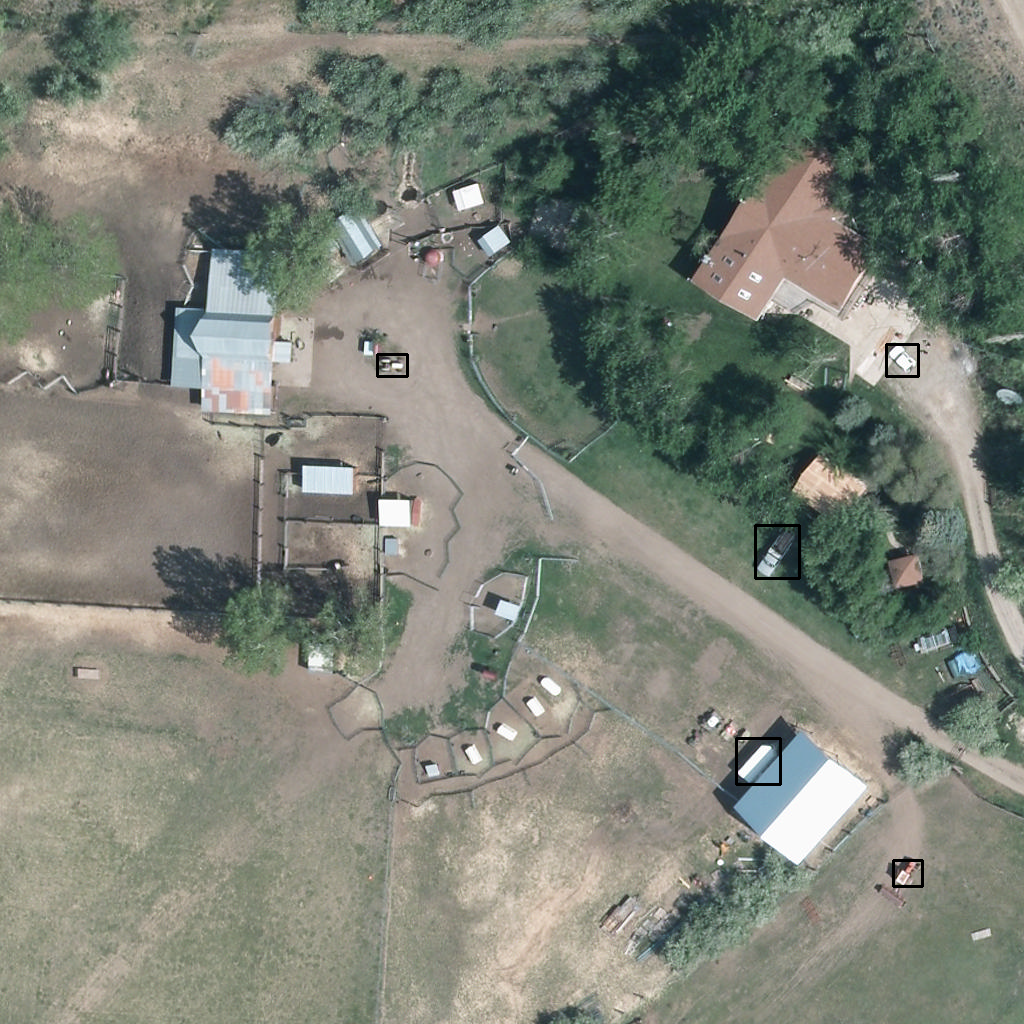
\includegraphics[trim={880pt 630pt 70pt 330pt},clip,width=\linewidth]{images/015Results/01abb_vs_obb/comp_images/ground_truth_abb/523.png}
    %Truck
    & \includegraphics[trim={360pt 200pt 540pt 715pt},clip,width=\linewidth]{images/015Results/01abb_vs_obb/comp_images/ground_truth_abb/212.png}
    %Camping Car
    & \includegraphics[trim={730pt 220pt 200pt 720pt},clip,width=\linewidth]{images/015Results/01abb_vs_obb/comp_images/ground_truth_abb/523.png}
    %Tractor
    & \includegraphics[trim={850pt 110pt 80pt 830pt},clip,width=\linewidth]{images/015Results/01abb_vs_obb/comp_images/ground_truth_abb/523.png}
    %Plane
    &  \includegraphics[trim={650pt 120pt 170pt 720pt},clip,width=\linewidth]{images/015Results/01abb_vs_obb/comp_images/ground_truth_abb/487.png}
    %Ship
    & \includegraphics[trim={230pt 200pt 680pt 725pt},clip,width=\linewidth]{images/015Results/01abb_vs_obb/comp_images/ground_truth_abb/509.png}
    %vehicle
    & \includegraphics[trim={440pt 360pt 460pt 555pt},clip,width=\linewidth]{images/015Results/01abb_vs_obb/comp_images/ground_truth_abb/427.png}
    %Pick Up
    & \includegraphics[trim={740pt 420pt 180pt 510pt},clip,width=\linewidth]{images/015Results/01abb_vs_obb/comp_images/ground_truth_abb/523.png}
    %Van
    & \includegraphics[trim={300pt 355pt 610pt 570pt},clip,width=\linewidth]{images/015Results/01abb_vs_obb/comp_images/ground_truth_abb/198.png} \\ \hline

    \rotatebox{90}{\textbf{\acrshort{GT} (\acrshort{obb})}} 
    %Car
    & \includegraphics[trim={880pt 630pt 70pt 330pt},clip,width=\linewidth]{images/015Results/01abb_vs_obb/comp_images/ground_truth_obb/523.png}
    %Truck
    & \includegraphics[trim={360pt 200pt 540pt 715pt},clip,width=\linewidth]{images/015Results/01abb_vs_obb/comp_images/ground_truth_obb/212.png}
    %Camping Car
    & \includegraphics[trim={730pt 220pt 200pt 720pt},clip,width=\linewidth]{images/015Results/01abb_vs_obb/comp_images/ground_truth_obb/523.png}
    %Tractor
    & \includegraphics[trim={850pt 110pt 80pt 830pt},clip,width=\linewidth]{images/015Results/01abb_vs_obb/comp_images/ground_truth_obb/523.png}
    %Plane
    &  \includegraphics[trim={650pt 120pt 170pt 720pt},clip,width=\linewidth]{images/015Results/01abb_vs_obb/comp_images/ground_truth_obb/487.png}
    %Ship
    & \includegraphics[trim={230pt 200pt 680pt 725pt},clip,width=\linewidth]{images/015Results/01abb_vs_obb/comp_images/ground_truth_obb/509.png}
    %vehicle
    & \includegraphics[trim={440pt 360pt 460pt 555pt},clip,width=\linewidth]{images/015Results/01abb_vs_obb/comp_images/ground_truth_obb/427.png}
    %Pick Up
    & \includegraphics[trim={740pt 420pt 180pt 510pt},clip,width=\linewidth]{images/015Results/01abb_vs_obb/comp_images/ground_truth_obb/523.png}
    %Van
    & \includegraphics[trim={300pt 355pt 610pt 570pt},clip,width=\linewidth]{images/015Results/01abb_vs_obb/comp_images/ground_truth_obb/198.png} \\ \hline
    \rotatebox{90}{\textbf{\acrshort{abb}}} 
    %Car
    & \includegraphics[trim={880pt 630pt 70pt 330pt},clip,width=\linewidth]{images/015Results/01abb_vs_obb/comp_images/abb/523.png}
    %Truck
    & \includegraphics[trim={360pt 200pt 540pt 715pt},clip,width=\linewidth]{images/015Results/01abb_vs_obb/comp_images/abb/212.png}
    %Camping Car
    & \includegraphics[trim={730pt 220pt 200pt 720pt},clip,width=\linewidth]{images/015Results/01abb_vs_obb/comp_images/abb/523.png}
    %Tractor
    & \includegraphics[trim={850pt 110pt 80pt 830pt},clip,width=\linewidth]{images/015Results/01abb_vs_obb/comp_images/abb/523.png}
    %Plane
    &  \includegraphics[trim={650pt 120pt 170pt 720pt},clip,width=\linewidth]{images/015Results/01abb_vs_obb/comp_images/abb/487.png}
    %Ship
    & \includegraphics[trim={230pt 200pt 680pt 725pt},clip,width=\linewidth]{images/015Results/01abb_vs_obb/comp_images/abb/509.png}
    %vehicle
    & \includegraphics[trim={440pt 360pt 460pt 555pt},clip,width=\linewidth]{images/015Results/01abb_vs_obb/comp_images/abb/427.png}
    %Pick Up
    & \includegraphics[trim={740pt 420pt 180pt 510pt},clip,width=\linewidth]{images/015Results/01abb_vs_obb/comp_images/abb/523.png}
    %Van
    & \includegraphics[trim={300pt 355pt 610pt 570pt},clip,width=\linewidth]{images/015Results/01abb_vs_obb/comp_images/abb/198.png} \\ \hline
    \rotatebox{90}{\textbf{\acrshort{obb}}} 
    %Car
    & \includegraphics[trim={880pt 630pt 70pt 330pt},clip,width=\linewidth]{images/015Results/01abb_vs_obb/comp_images/obb/523.png}
    %Truck
    & \includegraphics[trim={360pt 200pt 540pt 715pt},clip,width=\linewidth]{images/015Results/01abb_vs_obb/comp_images/obb/212.png}
    %Camping Car
    & \includegraphics[trim={730pt 220pt 200pt 720pt},clip,width=\linewidth]{images/015Results/01abb_vs_obb/comp_images/obb/523.png}
    %Tractor
    & \includegraphics[trim={850pt 110pt 80pt 830pt},clip,width=\linewidth]{images/015Results/01abb_vs_obb/comp_images/obb/523.png}
    %Plane
    &  \includegraphics[trim={650pt 120pt 170pt 720pt},clip,width=\linewidth]{images/015Results/01abb_vs_obb/comp_images/obb/487.png}
    %Ship
    & \includegraphics[trim={230pt 200pt 680pt 725pt},clip,width=\linewidth]{images/015Results/01abb_vs_obb/comp_images/obb/509.png}
    %vehicle
    & \includegraphics[trim={440pt 360pt 460pt 555pt},clip,width=\linewidth]{images/015Results/01abb_vs_obb/comp_images/obb/427.png}
    %Pick Up
    & \includegraphics[trim={740pt 420pt 180pt 510pt},clip,width=\linewidth]{images/015Results/01abb_vs_obb/comp_images/obb/523.png}
    %Van
    & \includegraphics[trim={300pt 355pt 610pt 570pt},clip,width=\linewidth]{images/015Results/01abb_vs_obb/comp_images/obb/198.png} \\ \hline
     \rotatebox{90}{\textbf{\acrshort{abb} in \acrshort{obb}}} 
    %Car
    & \includegraphics[trim={880pt 630pt 70pt 330pt},clip,width=\linewidth]{images/015Results/01abb_vs_obb/comp_images/aab_old/523.png}
    %Truck
    & \includegraphics[trim={360pt 200pt 540pt 715pt},clip,width=\linewidth]{images/015Results/01abb_vs_obb/comp_images/aab_old/212.png}
    %Camping Car
    & \includegraphics[trim={730pt 220pt 200pt 720pt},clip,width=\linewidth]{images/015Results/01abb_vs_obb/comp_images/aab_old/523.png}
    %Tractor
    & \includegraphics[trim={850pt 110pt 80pt 830pt},clip,width=\linewidth]{images/015Results/01abb_vs_obb/comp_images/aab_old/523.png}
    %Plane
    &  \includegraphics[trim={650pt 120pt 170pt 720pt},clip,width=\linewidth]{images/015Results/01abb_vs_obb/comp_images/aab_old/487.png}
    %Ship
    & \includegraphics[trim={230pt 200pt 680pt 725pt},clip,width=\linewidth]{images/015Results/01abb_vs_obb/comp_images/aab_old/509.png}
    %vehicle
    & \includegraphics[trim={440pt 360pt 460pt 555pt},clip,width=\linewidth]{images/015Results/01abb_vs_obb/comp_images/aab_old/427.png}
    %Pick Up
    & \includegraphics[trim={740pt 420pt 180pt 510pt},clip,width=\linewidth]{images/015Results/01abb_vs_obb/comp_images/aab_old/523.png}
    %Van
    & \includegraphics[trim={300pt 355pt 610pt 570pt},clip,width=\linewidth]{images/015Results/01abb_vs_obb/comp_images/aab_old/198.png} \\ \hline
\end{tabularx}
\caption[aab and obb: Examples of different classes for the object recognition performance]{Examples of different classes for the object recognition performance of different bounding box formats. The numbers displayed on the bounding boxes indicate the confidence of the model in the classification of the respective box. For Color Scheme explanation see Tab. \ref{tab:class_colors}}.
\label{fig:aab_obb_example_pics}
\end{figure}
\FloatBarrier

%%%%%%%%%%%%%%%%%%%%%%%%%%%%%%%%%%%%%%%%%%%%%%%%%%%%%%%%%%%%%%%%%%%%%%%%%%%%%%%%%%%%%%%%%%%%%%%%%%%%%%%%%%%%%%%%%%%%%%%%%%%%%%%%%%%%%%%%%%%%%%%%%%%%%%%%%%%%%%%%%%%%%%%%%%%%%%%%%%%%%%%%%%%%%%%%%%%%%%%%%%%%%%%%%%%%%%%%%%%%%%%%%
% \subsection{Comparision with Confusion Matrices}
% \todo{Beschreibung Figures länger machen, mehr analyse weniger "was sieht man"}
% \begin{figure}[htbp]
%     \centering
%     \includesvg[width=0.9\textwidth]{images/015Results/02perm_exp/confusion_matrices/rgbir_F2.svg}
%     \caption[Confusion Matrix for RGBIR Modell (Fold 2)]{Confusion Matrix for RGBIR Modell (Fold 2) .(Own representation)}
%     \label{fig:perm_exp_confM_rgbir_f2}
% \end{figure}
% \begin{itemize}
%     \item exatk bei planes (100\%)
%     \item hervoragende Performance (>80\%) bei Cars, Ships, Tractors, Planes
%     \item gute Performance (>60\% und <80 \%  ) bei Truck, Camping Car, van und Pick Up
%     \item akzeptable Performance  (> 60\%)bei vehicle
%     \item Background wird oft als Vehicle fehlklassifiziert (>40\%), Cmaping Car liegt bei (28\%), Truck bei 16\%. Rest in einer spanne von 8-12\%
% \end{itemize}
% \begin{itemize}
%     \item \ref{fig:perm_exp_confM_rgbir_f2} ist basis für Differenzmatrixen, weil es das beste Modell des Permuationsdurchlauf des \acrshort{RGBIR} Durchlaufes ist. Dieser Durchlauf wird gewählt weil er alle vorhanden Bänder unverändert in Rohform enthält
%     \item Interpretation der folgenden Differenzmatrixen wie folgt: Rot für bessere Performance des RGBIR (F2) Modells und Blau für das jeweils andere. Je satter die Farbe desto extremer der Unterschied
%     \item Vergleich fängt mit schlechtestem Modell an und arbeitet sich zum besten Modell laut oberen Whisker von Abb. \ref{fig:perm_exp_map50-95:val_on_test} hoch 
%     \item Unterschied (in \% von der Referenz)	Kategorie
%     \item 0 – 5 \%	gering
%     \item 5 – 10 \%	moderat/mittel
%     \item 10 – 20 \%	hoch
%     \item > 20 \%	sehr hoch
% \end{itemize}

% \begin{table}[h!]
% \centering
% \begin{tabular}{c c}
% \hline
% \textbf{Difference (in \% from reference)} & \textbf{Category} \\ \hline
% 0 -- 5 \%   & low \\ 
% 5 -- 10 \%  & moderate \\ 
% 10 -- 20 \% & high \\ 
% > 20 \%     & very high \\ \hline
% \end{tabular}
% \caption{Classification of differences relative to the reference}
% \end{table}


% \begin{figure}[htbp]
%     \centering
%     \includesvg[width=0.9\textwidth]{images/015Results/02perm_exp/confusion_matrices/Difference_Matrices/RGBIR_F2_vs_RGBNDVI_F2.svg}
%     \caption[Difference Matrix for RGBNDVI (Fold 2)]{Difference Matrix for RGBNDVI (Fold 2).(Own representation)}
%     \label{fig:perm_exp_diffM_rgbndvi_f2}
% \end{figure}
% \begin{itemize}
%     \item hohe Unterschiede (>10\%) bei Verwechselung von Car und Van zugunsten RGBIR
%     \item hohe bis sehr hohe Unterschiede bei der (richtigen) Erkennungsleistung von Ship (24\%), Vehicle (16\%), Plane (12\%) und Tractor (10\%) zugunsten RGBIR
%     \item restliche Unterschiede bei Verwechslungen von Detekionen im geringen (0-5\%) und moderaten (5-10\%) Bereich
%     \item Plane (12\%) und van (23\%)  wird oft als background fehlklassifiziert; restliche fehlklassifizierungen liegen im geringen bis mittleren Bereich zulasten von RGBNDVI
%     \item Insgesamt: 5x RGBIR mind. 5\% besser (diagonale der CM), 0x blau
% \end{itemize}

% \begin{figure}[htbp]
%     \centering
%     \includesvg[width=0.9\textwidth]{images/015Results/02perm_exp/confusion_matrices/Difference_Matrices/RGBIR_F2_vs_GBNDVI_F2.svg}
%     \caption[Difference Matrix for GBNDVI (Fold 2)]{Difference Matrix for GBNDVI (Fold 2).(Own representation)}
%     \label{fig:perm_exp_diffM_gbndvi_f2}
% \end{figure}
% \begin{itemize}
%     \item sehr hohe Unterschiede zugunsten RGBIR bei richtiger Erkennungsleistung von Tractor
%     \item Ship hat "nur" eine bessere Leistung von 8\% anstatt 24\%
%     \item Tractor, Ship, van wird öfters als Background fehlklassifiziert
%     \item Insgesamt: 4x RGBIR mind. 5\% besser (diagonale CM) 0x blau
% \end{itemize}

% \begin{figure}[htbp]
%     \centering
%     \includesvg[width=0.9\textwidth]{images/015Results/02perm_exp/confusion_matrices/Difference_Matrices/RGBIR_F2_vs_IRGB_F3.svg}
%     \caption[Difference Matrix for IRGB (Fold 3)]{Difference Matrix for IRGB (Fold 3).(Own representation)}
%     \label{fig:perm_exp_diffM_irgb_f3}
% \end{figure}
% \begin{itemize}
%     \item Ship hat wieder eine bessere Leistung von 21\%
%     \item Ship wird oft als Campoing Car missclassifiziert
%     \item Ship wird oft als Background nicht erkannt
%     \item Insgesamt: 3x RGBIR mind. 5\% besser (diagonale CM) 0x blau
% \end{itemize}

% \begin{figure}[htbp]
%     \centering
%     \includesvg[width=0.9\textwidth]{images/015Results/02perm_exp/confusion_matrices/Difference_Matrices/RGBIR_F2_vs_RIRB_F2.svg}
%     \caption[Difference Matrix for RIRB (Fold 2)]{Difference Matrix for RIRB (Fold 2).(Own representation)}
%     \label{fig:perm_exp_diffM_RIRB_f2}
% \end{figure}
% \begin{itemize}
%     \item MOderate Verwechslung von Van als Car (9 \%)
%     \item hoher Unterschied bei Ship und van Klassifizierung
%     \item moderat bessere Leistung zugunsten RIRB bei Camping Car (6\%)
%     \item hohe Fehldetektion von RIRB von Van als Background (21\%); 12 \% bei Ship
%     \item moderate bessere Leistung von RGBIR bei Vehicle, camping car in bezug auf Verwechlseung Background/label
%     \item Insgesamt: 2x RGBIR mind. 5\% besser (diagonale CM) 1x blau
% \end{itemize}

% \begin{figure}[htbp]
%     \centering
%     \includesvg[width=0.9\textwidth]{images/015Results/02perm_exp/confusion_matrices/Difference_Matrices/RGBIR_F2_vs_RGB_F2.svg}
%     \caption[Difference Matrix for RGB (Fold 2)]{Difference Matrix for RGB (Fold 2).(Own representation)}
%     \label{fig:perm_exp_diffM_RGB_f2}
% \end{figure}
% \begin{itemize}
%     \item hohe Unterschiede zugnsten RGBIR bei Ship, und Vehicle Detektion
%     \item moderate VErwechslungen von Pick up mit Cars (6\%) und vans mit pck ups bei RGBIR
%     \item Background wird oft (7\%) häufiger als Pick up identifiziert von RGBIR
%     \item RGB erkennt Vehicle (15\%) und Ship (10\%) oft als Background
%     \item Insgesamt: 2x RGBIR mind. 5\% besser (diagonale CM) 0x blau
% \end{itemize}
% \begin{figure}[htbp]
%     \centering
%     \includesvg[width=0.9\textwidth]{images/015Results/02perm_exp/confusion_matrices/Difference_Matrices/RGBIR_F2_vs_RGIR_F3.svg}
%     \caption[Difference Matrix for RGIR (Fold 3)]{Difference Matrix for RGIR (Fold 3).(Own representation)}
%     \label{fig:perm_exp_diffM_RGIR_f3}
% \end{figure}
% \begin{itemize}
%     \item cars werden öfter mit van verwecheslt von rgbir
%     \item camping car wird öfter von rgbir als Background klassifiziert als bei rgir
%     \item bei ship und van ist rgir moderat besser
%     \item Insgesamt: 1x RGBIR mind. 5\% besser (diagonale CM) 1x blau (nahezu gleihcstand)
% \end{itemize}

%%%%%%%%%%%%%%%%%%%%%%%%%%%%%%%%%%%%%%%%%%%%%%%%%%%%%%%%%%%%%%%%%%%%%%%%%%%%%%%%%%%%%%%%%%%%%%%%%%%%%%%%%%%%%%%%%%%%%%%%%%%%%%%%%%%%%%%%%%%%%%%%%%%%%%%%%%%%%%%%%%%%%%%%%%%%%%%%%%%%%%%%%%%%%%%%%%%%%%%%%%%%%%%%%%%%%%%%%%%%%%%%%%%%%%%%%%%%%%%%%%%%%%%%%%%%%%%%%%%%%%%%%%%%%%%%%%%%%%%%%%%%%%%%%%%%%%%%%%%%%%%%%%%%%%%%%%%%%%%%%%%%%%%%%%%%%%%%%%%%%%%%%%%%%%%%%%%%%%%%%%%%%%%%%%%%%%

% \begin{itemize}
%     \item \todo{beide confusionsmatricen einfügen}
%     \item Normalisierte Konfusions Matrix mit 9 Klassen und der Einteilung Background (Hintergrund)
%     \item Right: Confusion Matric of RGBIR Modell on Fold 2:
%     \item Good Performance at Cars, Trucks, Ships, Tractors, Camping Cars, Pick Up and planes
%     \item Many confusion at vehicle with background
%     \item Nearly the same for RGIR at Fold 3
%     \item Both modells detected nearly all Planes
%     \item Difference Matrics at next slide
% \end{itemize}

% \begin{itemize}
%     \item \todo{Differenzmatrix RGBIR vs RGIR einfügen}
%     \item At all Difference Matrices is red for the better performance of the RGBIR Model and blue for the other modell
%     \item RGBIR detected Trucks, Ships and Tractor more accurate than the RGIR Model
%     \item RGBIR seems more robust for common ground vehicles
%     \item Both modells detect all planes (in short every modell detect all planes)
%     \item Both modells misclassifier background as any class (RGBIR is better at vehicle and Camping Car) 
% \end{itemize}

% \begin{itemize}
%     \item \todo{Differenzmatrix RGBIR vs RGB einfügen}
%     \item RGBIR is better for detecting Ships (12\%) and Vehicles (15\%), slightliy degrades performance of car detection
%     \item Vehicle is much better than in RGB Model (15\%)
%     \item IR input helps for common vehicle recognition (vehicle includes Excavators, construction equipment, etc.)
%     \item RGB is better in identifying ship and vehicle as background
% \end{itemize}


% \begin{itemize}
%     \item \todo{Differenzmatrix RGBIR vs IRGB einfügen}
%     \item RGBIR recognize Ships 21 \% better than the irgb model
%     \item Particulary stronger for camping car and van classification (6\%)
%     \item IRGB has more  background-ship and background-vehicle confusion
% \end{itemize}

% \begin{itemize}
%     \item \todo{Differenzmatrix RGBIR vs RIRB einfügen}
%     \item RGBIR detects Ships and vans better than RIRB Model
%     \item RIRB misclassified van and ship as background more often than RGBIR

% \end{itemize}


% \begin{itemize}
%     \item \todo{Differenzmatrix RGBIR vs GBNDBVI und RGBNDVI einfügen}
%     \item RGBIR have a better performance in Ship, Tractor and Vehicle
%     \item Both ndvi modells show  a tendency for confusing background with other classes
% \end{itemize}


%##########################################################################
%##########################################################################
%##########################################################################
%##########################################################################
%##########################################################################
%##########################################################################
%##########################################################################
%##########################################################################
%##########################################################################
\section{Ablation Studies}
% \begin{itemize}
%     \item Fold 4 und 2 am besten bei vali datensatz
%     \item Fold 0,2,3 bei test datensatz
% \end{itemize}
% \begin{itemize}
%     \item ir ist am besten mit höchstem Map wert
% \end{itemize}
Die Boxplots in Fig. \ref{fig:ablation_map50-95:val_on_test} der 6-fold Cross-Validation zeigen, dass die Modelle für die Kanäle Red, Green, Blue und IR im Bereich von mAP50–95 = 0,52–0,54 liegen. Ein einzelner Wert im IR-Modell erreicht 0,5777, liegt damit jedoch deutlich außerhalb des zentralen Bereichs der anderen Folds und ist als Ausreißer zu interpretieren. Insgesamt lassen sich zwischen den Modellen Red, Green, Blue und IR keine signifikanten Unterschiede feststellen, während NDVI mit einem Median von etwa 0,44 signifikant schlechter abschneidet. Ähnliche Ergebnisse sind in Fig. \ref{fig:ablation_map50-95:val_on_val} zu sehen.

Die Auswertung der Ergebnisse in \ref{tab:ablation_best_folds_test}zeigt außerdem, dass insbesondere Fold~4 und Fold~2 die besten Resultate auf dem Validierungsdatensatz erzielen konnten. Auf dem Testdatensatz hingegen erreichen die Folds~0, 2 und~3 die besten Leistungen.  

Insgesamt weist das IR-Modell die höchste Performance auf und erzielt den höchsten \acrshort{mAP}-Wert im Vergleich zu den anderen untersuchten Varianten.  




\begin{figure}[htbp]
    \centering
    \includesvg[width=0.8\textwidth]{images/015Results/03ablation/best_val_on_test.svg}
    \caption[Comparison of \acrshort{mAP}50-95 values for channels: red, green, blue, ndvi (Best validation model on test dataset)]{Comparison of \acrshort{mAP}50-95 values for channels: red, green, blue, ndvi (Best validation model on test dataset). The red dot is the fold, that has the best \acrshort{mAP}50-95 at the validation dataset (see fig. \ref{fig:ablation_map50-95:val_on_val}).(Own representation)}
    \label{fig:ablation_map50-95:val_on_test}
\end{figure}


\begin{figure}[htbp]
    \centering
    \includesvg[width=0.8\textwidth]{images/015Results/03ablation/best_val_on_val.svg}
    \caption[Comparison of \acrshort{mAP}50-95 values for channels: red, green, blue, ndvi (Best validation model on validation dataset)]{Comparison of \acrshort{mAP}50-95 values for channels: red, green, blue, ndvi (Best validation model on validation dataset). (Own representation)}
    \label{fig:ablation_map50-95:val_on_val}
\end{figure}

\begin{figure}[htbp]
    \centering
    % Erste Spalte
       
    \begin{subfigure}{0.48\textwidth}
        \centering
        \includesvg[width=\linewidth]{images/015Results/03ablation/conf_matr_ir_f0.svg}
        \caption{IR (F3)}
        \label{fig:ablation_confM_IR_f0}
    \end{subfigure}

    \begin{subfigure}{0.48\textwidth}
        \centering
        \includesvg[width=\linewidth]{images/015Results/03ablation/diff_matric/IR_F0_vs_R_F2.svg}
        \caption{Red (F2)}
        \label{fig:ablation_diffM_r_f2}
    \end{subfigure}
    \begin{subfigure}{0.48\textwidth}
        \centering
        \includesvg[width=\linewidth]{images/015Results/03ablation/diff_matric/IR_F0_vs_G_F3.svg}
        \caption{Green (F3)}
        \label{fig:ablation_diffM_g_f3}
    \end{subfigure}
    
    \begin{subfigure}{0.48\textwidth}
        \centering
        \includesvg[width=\linewidth]{images/015Results/03ablation/diff_matric/IR_F0_vs_B_F2.svg}
        \caption{Blue (F2)}
        \label{fig:ablation_diffM_b_f2}
    \end{subfigure}
    \begin{subfigure}{0.48\textwidth}
        \centering
        \includesvg[width=\linewidth]{images/015Results/03ablation/diff_matric/IR_F0_vs_NDVI_F0.svg}
        \caption{NDVI (F0)}
        \label{fig:ablation_diffM_NDVI_f0}
    \end{subfigure}
    


    \caption[Confusion Matrix for IR Model at Fold 3 and the Difference Matrices compared to this Model]{Confusion Matrix for IR Model at Fold 3 and the Difference Matrices compared to this Model. Red indicates better performance for IR, blue for the respective comparison model. All values falling within the interval [–0.05, 0.05] are excluded from the matrices.}
    \label{fig:ablation_diffM_all}
\end{figure}

Im Anschluss an die Analyse der Permutations-Experimente (vgl. Abschnitt \ref{subsec:permexp_comp_confusion_matric}) wird nun die Klassifikationsleistung der Modelle unter Verwendung der Confusion Matrix des IR-Modells als Referenz untersucht (siehe Abbildung \ref{fig:ablation_confM_IR_f0}). Die Auswertung erfolgt analog zur Kategorisierung der Unterschiede in Tabelle \ref{tab:diff_cat}.  

Das IR-Modell zeigt eine perfekte Erkennungsrate von 100\,\% bei der Klasse \textit{Plane}. Sehr hohe Erkennungsraten von über 80\,\% konnten zudem für die Klassen \textit{Car} und \textit{Tractor} erzielt werden, was auf eine insgesamt hervorragende Klassifikationsleistung in diesen Kategorien hinweist.  

Eine gute Performance mit Erkennungsraten zwischen 60\,\% und 80\,\% wurde für die Klassen \textit{Truck}, \textit{Ship}, \textit{Camping Car} sowie \textit{Pick Up} erreicht. Demgegenüber liegen die Erkennungsraten für die Klassen \textit{Van} und \textit{Vehicle} im Bereich von 40--60\,\%, was lediglich eine moderate Klassifikationsleistung darstellt.  

Auffällig ist insbesondere die fehlerhafte Klassifikation der Klasse \textit{Vehicle}, die in 45\,\% der Fälle dem \textit{Background} zugeordnet wurde. Darüber hinaus treten erhöhte Fehlklassifikationen in mehreren weiteren Kategorien auf: \textit{Pick Up}, \textit{Ship}, \textit{Camping Car} (28\,\%) sowie \textit{Van} (39\,\%) weisen besonders hohe Raten an Fehlzuordnungen auf. Diese Ergebnisse verdeutlichen die spezifischen Schwächen des IR-Modells im Vergleich zu den in den Permutations-Experimenten untersuchten Varianten.  


% \begin{itemize}
%     \item Beschreibung der Differenzmatrixen erfolgt analog zu Kap. \ref{subsec:permexp_comp_confusion_matric} und Tab. \ref{tab:diff_cat} mit der Confusion Matrix IR (s. Fig. \ref{fig:ablation_confM_IR_f0}) als Referenz
%     \item ebenfalls perfekte Erkennungsrate von 100 \% bei planes
%     \item >80\%: Car, Tractor (hervorragend)
%     \item 60-80\% Truck, Ship, Camping Car, Pick Up (gut)
%     \item 40-60\%: van, Vehicle
%     \item nicht erkennung von vehicle (als Background) mit 45 \% häufig
%     \item erhöhte Fehlklassifikationen (>17\%) ebenfalls bei Pick UP, Ship, Camping Car (28\%) und van (39 \%)
% \end{itemize}
Die Analyse der Differenzmatrizen verdeutlicht die jeweilige Bedeutung einzelner Kanäle im Vergleich zum IR-Referenzmodell (vgl. Abbildung \ref{fig:ablation_confM_IR_f0}).  

Abbildung \ref{fig:ablation_diffM_r_f2} zeigt, dass IR eine deutlich höhere Leistung bei der Erkennung der Klasse \textit{Vehicle} im Vergleich zum reinen roten Kanal aufweist. Für die Klasse \textit{Van} erweist sich hingegen der rote Kanal als vorteilhaft, da er hier eine um 16\,\% höhere Erkennungsrate erzielt. Das IR-Modell zeigt dagegen Vorteile bei der Klassifikation von \textit{Van} (12\,\%), \textit{Camping Car} (9\,\%) sowie moderat bei \textit{Pick Up} (6\,\%).  

In Abbildung \ref{fig:ablation_diffM_g_f3} wird der Vergleich mit dem grünen Kanal dargestellt. Hier erzielt der grüne Kanal eine deutlich höhere Leistung bei der Erkennung von \textit{Ship} (26\,\%) sowie eine hohe Verbesserung bei \textit{Van} (17\,\%). Das IR-Modell ist dagegen bei der Erkennung von \textit{Truck} (14\,\%) überlegen. Besonders auffällig ist die Unterscheidung von Objekten gegenüber dem Hintergrund: Hier weist IR bei \textit{Van} mit 25\,\% eine deutlich bessere Leistung auf. Auch bei \textit{Ship} und \textit{Vehicle} erreicht IR eine hohe Präzision, während bei \textit{Camping Car} (8\,\%) und \textit{Pick Up} (6\,\%) moderate Vorteile bestehen. Demgegenüber zeigt der grüne Kanal bessere Resultate bei \textit{Truck} (15\,\%) und moderat bei \textit{Tractor} (6\,\%). Bei der Klasse \textit{Car} ergibt sich kein signifikanter Unterschied. Insgesamt ist IR in sieben Fällen mindestens 5\,\% besser, während der grüne Kanal in sechs Fällen Vorteile aufweist.  

Abbildung \ref{fig:ablation_diffM_b_f2} stellt den Vergleich mit dem blauen Kanal dar. Dieser zeigt moderate Vorteile bei \textit{Camping Car} und \textit{Pick Up} sowie eine deutliche Verbesserung bei \textit{Van} (13\,\%). Das IR-Modell ist hingegen bei \textit{Truck} (10\,\%) sowie moderat bei \textit{Ship} und \textit{Vehicle} (je 9\,\%) überlegen. Zudem gelingt es IR, \textit{Van} besser vom Hintergrund zu unterscheiden (10\,\%) und moderate Vorteile bei \textit{Camping Car} (6\,\%) sowie \textit{Pick Up} (5\,\%) zu erzielen. Der blaue Kanal zeigt hingegen moderate Verbesserungen bei der Unterscheidung von \textit{Truck} und \textit{Vehicle} gegenüber dem Hintergrund. Insgesamt ist IR in sechs Fällen klar überlegen, während der blaue Kanal in fünf Fällen Vorteile aufweist.  

Im Vergleich mit NDVI weist IR eine höhere Präzision bei den Klassen \textit{Car}, \textit{Truck}, \textit{Tractor} sowie \textit{Camping Car} auf und ist insbesondere bei \textit{Ship} (24\,\%) deutlich exakter. Auch bei \textit{Vehicle} erreicht IR eine moderate Verbesserung (6\,\%). NDVI zeigt dagegen Vorteile bei der Unterscheidung von Hintergrund und Objekt, insbesondere moderat bei \textit{Truck} und \textit{Camping Car}, sowie eine höhere Präzision bei \textit{Ship} (26\,\%) und \textit{Tractor} (13\,\%). Insgesamt ist IR in sieben Fällen mindestens 5\,\% besser als NDVI, während NDVI lediglich in vier Fällen Vorteile bei der Hintergrund-Objekt-Unterscheidung aufweist.  

Zusammenfassend lässt sich festhalten, dass sämtliche Modelle – mit Ausnahme des NDVI-Modells – eine hohe Klassifikationsleistung in der Kategorie \textit{Car} aufweisen, was sich auch in den Beispielabbildungen deutlich widerspiegelt (vgl. Abbildung \ref{fig:ablation_example_pics}). Gleichzeitig zeigen sowohl die Differenzmatrizen als auch die Abbildungen, dass Fehlklassifikationen zwischen Hintergrund und Objekt weiterhin in erheblichem Maße auftreten, insbesondere innerhalb der Klasse \textit{Vehicle} (vgl. Confusion Matrix \ref{fig:ablation_confM_IR_f0}). Auffällig ist hierbei der IR-Kanal, der in dem in Abbildung \ref{fig:ablation_example_pics} dargestellten Beispielen eine besonders hohe Verwechslungsrate zwischen Objekten und Hintergrund aufweist, während in den übrigen Kanälen insgesamt mehr Objekte korrekt erkannt werden. Darüber hinaus wird die Verwechslung der Klasse \textit{Van} mit \textit{Car} im Red-Modell in der Differenzmatrix \ref{fig:ablation_diffM_g_f3} bestätigt. Im Vergleich zum Referenzmodell (6\,\%, vgl. Abbildung \ref{fig:ablation_confM_IR_f0}) ist hierbei weder eine Leistungssteigerung noch eine Verschlechterung festzustellen. Das NDVI-Modell weist hingegen eine deutlich reduzierte Leistungsfähigkeit auf: In dAbbildung \ref{fig:ablation_example_pics} wird sichtbar, dass – mit Ausnahme der korrekten Klassifikation von \textit{Van} sowie der Fehlklassifikation von \textit{Truck} als \textit{Vehicle} – keine zutreffenden Ergebnisse erzielt wurden. Sämtliche weiteren Klassen wurden fälschlicherweise dem Hintergrund zugeordnet.




% \begin{itemize}
%     \item \ref{fig:ablation_diffM_r_f2} zeigt, dass IR  hohe Leistung im Gegensatz zm reinen Roten Kanal bei der Erkennung von Vehicle hat
%     \item dafür scheint IR Bei der Erkennung von Vans nicht wichtig zu sein, R war 16 \% besser als IR
%     \item Ir war deutlich besser bei der erkenung von vans (12 \%) und camping cars (9 \%), moderat bei pick Up (6\%)
% \end{itemize}
% \begin{itemize}
%     \item \ref{fig:ablation_diffM_g_f3} zeigt das Green bei Shipdetection eine deutlich höhere Leistung (26\%) erbracht hat, hoch war die Leistung auhc bei vans (17 \%)
%     \item IR war dagegen bei Trucks (14\%) besser 
%     \item bei der Untershciedung von Objekt zu Hintergrund war IR bei van mit 25\% deutlihc besser; hohe Leistung bei Ship und Vehicle und moderate bessere Leistung bei Camping Car (8\%) und pick up (6\%)
%     \item bei Truck war Green deutlich bessser (15\%), bei Tractor Moderat (6\%)
%     \item kein signifikanter Unterschied bei Car Detection
%     \item insgesamt war ir 7x besser, green 6x (beides mind 5 \% besser)
% \end{itemize}
% \begin{itemize}
%     \item \ref{fig:ablation_diffM_b_f2} zeigt den blauen Kanal
%     \item blue schneidet moderat besser bei Camping Car und Pick up sowie deutlich besser bei van (13 \%) ab.
%     \item ir ist besser bei truck 10 \%, moderat besser bei ship und vehicle (9\%) 
%     \item IR kann besser van von hintergrund unterscheiden (10 \%) und moderat besser camping car 6\%  udn pick up 5 \%
%     \item blue ist moderat besser bei Truck und vehicle  von Hintergrund 
%     \item ingesatm ist ir 6x besser als blue, blue ist 5x besser als ir
% \end{itemize}
% \begin{itemize}
%     \item IR hat eine höhere Präzision bei Car, Truck, Tractor, Camping Car und ist deutlich exakter bei Ship (24\%); moderat besser bei vehicle (6 \%)
%     \item ndvi kann besser hintergrund von Objekt untershceiden (moderat bie Truck und Cmaping Car); höhere Präzision bei Ship (26\%) und Tractor (13\%)
%     \item insgesamt: ir 7x mind. 5\% besser als ndvi, ndvi nru bei hintergrund von objekt unterschiedung 4x 
% \end{itemize}
% \begin{itemize}
%     \item insgesamt ist die gute Leistung aller Modelle bei der Car Klassifizierung in Fig \ref{fig:ablation_example_pics} zu sehen
%     \item Verwechselung von Backgroudn mit Objekt (beispielhaft Truck oder ship) ist auch in der Differencmatrix \ref{fig:ablation_diffM_b_f2} für Blue und IR (s. Confusionmatrix \ref{fig:ablation_confM_IR_f0}) zu sehen
%     \item Verwechslung von Vehicle mit Truck von Green Model ist auch in Differencmatrix \ref{fig:ablation_diffM_g_f3} zu sehen
%     \item NDVI Modell schneidet auch in Beispielbildern sehr schlehct ab, Truck und SHip werden nicht erkannt, Pick up wird doppelt als Pick up und Car klassifiziert und Vehicle mit Truck verwechselt
% \end{itemize}
\begin{table}[h]
\centering
\begin{tabular}{l c c}
\hline
\textbf{Channel} & \textbf{Best mAP Fold (Validation)} & \textbf{Best mAP Fold (Test)} \\ 
\hline
red   & 4 & 2 (0.5408) \\
green & 4 & 3 (0.5449) \\
blue  & 4 & 2 (0.5449) \\
ir    & 4 & 0 (0.5777) \\
ndvi  & 2 & 0 (0.4467) \\
\hline
\end{tabular}
\caption{Best fold per model on validation and test sets, with test mAP@50-95 values}
\label{tab:ablation_best_folds_test}
\end{table}

\begin{figure}[h!]
\centering
\renewcommand{\arraystretch}{1.2} % mehr Platz zwischen Zeilen
\setlength{\tabcolsep}{2pt} % weniger Platz zwischen Spalten
\begin{tabularx}{\textwidth}{c|*{9}{X}}
    & \textbf{Car}
    & \textbf{Truck}
    & \textbf{Camping Car}
    & \textbf{Tractor}
    & \textbf{Plane}
    & \textbf{Ship}
    & \textbf{Vehicle}
    & \textbf{Pick-Up}
    & \textbf{Van} \\ \hline
    \rotatebox{90}{\textbf{\acrshort{GT} (\acrshort{abb})}} 
    %Car
    & \includegraphics[trim={880pt 630pt 70pt 330pt},clip,width=\linewidth]{images/015Results/01abb_vs_obb/comp_images/ground_truth_abb/523.png}
    %Truck
    & \includegraphics[trim={360pt 200pt 540pt 715pt},clip,width=\linewidth]{images/015Results/01abb_vs_obb/comp_images/ground_truth_abb/212.png}
    %Camping Car
    & \includegraphics[trim={730pt 220pt 200pt 720pt},clip,width=\linewidth]{images/015Results/01abb_vs_obb/comp_images/ground_truth_abb/523.png}
    %Tractor
    & \includegraphics[trim={850pt 110pt 80pt 830pt},clip,width=\linewidth]{images/015Results/01abb_vs_obb/comp_images/ground_truth_abb/523.png}
    %Plane
    &  \includegraphics[trim={650pt 120pt 170pt 720pt},clip,width=\linewidth]{images/015Results/01abb_vs_obb/comp_images/ground_truth_abb/487.png}
    %Ship
    & \includegraphics[trim={230pt 200pt 680pt 725pt},clip,width=\linewidth]{images/015Results/01abb_vs_obb/comp_images/ground_truth_abb/509.png}
    %vehicle
    & \includegraphics[trim={440pt 360pt 460pt 555pt},clip,width=\linewidth]{images/015Results/01abb_vs_obb/comp_images/ground_truth_abb/427.png}
    %Pick Up
    & \includegraphics[trim={740pt 420pt 180pt 510pt},clip,width=\linewidth]{images/015Results/01abb_vs_obb/comp_images/ground_truth_abb/523.png}
    %Van
    & \includegraphics[trim={300pt 355pt 610pt 570pt},clip,width=\linewidth]{images/015Results/01abb_vs_obb/comp_images/ground_truth_abb/198.png} \\ \hline

    \rotatebox{90}{\textbf{\acrshort{GT} (\acrshort{obb})}} 
    %Car
    & \includegraphics[trim={880pt 630pt 70pt 330pt},clip,width=\linewidth]{images/015Results/01abb_vs_obb/comp_images/ground_truth_obb/523.png}
    %Truck
    & \includegraphics[trim={360pt 200pt 540pt 715pt},clip,width=\linewidth]{images/015Results/01abb_vs_obb/comp_images/ground_truth_obb/212.png}
    %Camping Car
    & \includegraphics[trim={730pt 220pt 200pt 720pt},clip,width=\linewidth]{images/015Results/01abb_vs_obb/comp_images/ground_truth_obb/523.png}
    %Tractor
    & \includegraphics[trim={850pt 110pt 80pt 830pt},clip,width=\linewidth]{images/015Results/01abb_vs_obb/comp_images/ground_truth_obb/523.png}
    %Plane
    &  \includegraphics[trim={650pt 120pt 170pt 720pt},clip,width=\linewidth]{images/015Results/01abb_vs_obb/comp_images/ground_truth_obb/487.png}
    %Ship
    & \includegraphics[trim={230pt 200pt 680pt 725pt},clip,width=\linewidth]{images/015Results/01abb_vs_obb/comp_images/ground_truth_obb/509.png}
    %vehicle
    & \includegraphics[trim={440pt 360pt 460pt 555pt},clip,width=\linewidth]{images/015Results/01abb_vs_obb/comp_images/ground_truth_obb/427.png}
    %Pick Up
    & \includegraphics[trim={740pt 420pt 180pt 510pt},clip,width=\linewidth]{images/015Results/01abb_vs_obb/comp_images/ground_truth_obb/523.png}
    %Van
    & \includegraphics[trim={300pt 355pt 610pt 570pt},clip,width=\linewidth]{images/015Results/01abb_vs_obb/comp_images/ground_truth_obb/198.png} \\ \hline
    \rotatebox{90}{\textbf{\acrshort{abb}}} 
    %Car
    & \includegraphics[trim={880pt 630pt 70pt 330pt},clip,width=\linewidth]{images/015Results/01abb_vs_obb/comp_images/abb/523.png}
    %Truck
    & \includegraphics[trim={360pt 200pt 540pt 715pt},clip,width=\linewidth]{images/015Results/01abb_vs_obb/comp_images/abb/212.png}
    %Camping Car
    & \includegraphics[trim={730pt 220pt 200pt 720pt},clip,width=\linewidth]{images/015Results/01abb_vs_obb/comp_images/abb/523.png}
    %Tractor
    & \includegraphics[trim={850pt 110pt 80pt 830pt},clip,width=\linewidth]{images/015Results/01abb_vs_obb/comp_images/abb/523.png}
    %Plane
    &  \includegraphics[trim={650pt 120pt 170pt 720pt},clip,width=\linewidth]{images/015Results/01abb_vs_obb/comp_images/abb/487.png}
    %Ship
    & \includegraphics[trim={230pt 200pt 680pt 725pt},clip,width=\linewidth]{images/015Results/01abb_vs_obb/comp_images/abb/509.png}
    %vehicle
    & \includegraphics[trim={440pt 360pt 460pt 555pt},clip,width=\linewidth]{images/015Results/01abb_vs_obb/comp_images/abb/427.png}
    %Pick Up
    & \includegraphics[trim={740pt 420pt 180pt 510pt},clip,width=\linewidth]{images/015Results/01abb_vs_obb/comp_images/abb/523.png}
    %Van
    & \includegraphics[trim={300pt 355pt 610pt 570pt},clip,width=\linewidth]{images/015Results/01abb_vs_obb/comp_images/abb/198.png} \\ \hline
    \rotatebox{90}{\textbf{\acrshort{obb}}} 
    %Car
    & \includegraphics[trim={880pt 630pt 70pt 330pt},clip,width=\linewidth]{images/015Results/01abb_vs_obb/comp_images/obb/523.png}
    %Truck
    & \includegraphics[trim={360pt 200pt 540pt 715pt},clip,width=\linewidth]{images/015Results/01abb_vs_obb/comp_images/obb/212.png}
    %Camping Car
    & \includegraphics[trim={730pt 220pt 200pt 720pt},clip,width=\linewidth]{images/015Results/01abb_vs_obb/comp_images/obb/523.png}
    %Tractor
    & \includegraphics[trim={850pt 110pt 80pt 830pt},clip,width=\linewidth]{images/015Results/01abb_vs_obb/comp_images/obb/523.png}
    %Plane
    &  \includegraphics[trim={650pt 120pt 170pt 720pt},clip,width=\linewidth]{images/015Results/01abb_vs_obb/comp_images/obb/487.png}
    %Ship
    & \includegraphics[trim={230pt 200pt 680pt 725pt},clip,width=\linewidth]{images/015Results/01abb_vs_obb/comp_images/obb/509.png}
    %vehicle
    & \includegraphics[trim={440pt 360pt 460pt 555pt},clip,width=\linewidth]{images/015Results/01abb_vs_obb/comp_images/obb/427.png}
    %Pick Up
    & \includegraphics[trim={740pt 420pt 180pt 510pt},clip,width=\linewidth]{images/015Results/01abb_vs_obb/comp_images/obb/523.png}
    %Van
    & \includegraphics[trim={300pt 355pt 610pt 570pt},clip,width=\linewidth]{images/015Results/01abb_vs_obb/comp_images/obb/198.png} \\ \hline
     \rotatebox{90}{\textbf{\acrshort{abb} in \acrshort{obb}}} 
    %Car
    & \includegraphics[trim={880pt 630pt 70pt 330pt},clip,width=\linewidth]{images/015Results/01abb_vs_obb/comp_images/aab_old/523.png}
    %Truck
    & \includegraphics[trim={360pt 200pt 540pt 715pt},clip,width=\linewidth]{images/015Results/01abb_vs_obb/comp_images/aab_old/212.png}
    %Camping Car
    & \includegraphics[trim={730pt 220pt 200pt 720pt},clip,width=\linewidth]{images/015Results/01abb_vs_obb/comp_images/aab_old/523.png}
    %Tractor
    & \includegraphics[trim={850pt 110pt 80pt 830pt},clip,width=\linewidth]{images/015Results/01abb_vs_obb/comp_images/aab_old/523.png}
    %Plane
    &  \includegraphics[trim={650pt 120pt 170pt 720pt},clip,width=\linewidth]{images/015Results/01abb_vs_obb/comp_images/aab_old/487.png}
    %Ship
    & \includegraphics[trim={230pt 200pt 680pt 725pt},clip,width=\linewidth]{images/015Results/01abb_vs_obb/comp_images/aab_old/509.png}
    %vehicle
    & \includegraphics[trim={440pt 360pt 460pt 555pt},clip,width=\linewidth]{images/015Results/01abb_vs_obb/comp_images/aab_old/427.png}
    %Pick Up
    & \includegraphics[trim={740pt 420pt 180pt 510pt},clip,width=\linewidth]{images/015Results/01abb_vs_obb/comp_images/aab_old/523.png}
    %Van
    & \includegraphics[trim={300pt 355pt 610pt 570pt},clip,width=\linewidth]{images/015Results/01abb_vs_obb/comp_images/aab_old/198.png} \\ \hline
\end{tabularx}
\caption[aab and obb: Examples of different classes for the object recognition performance]{Examples of different classes for the object recognition performance of different bounding box formats. The numbers displayed on the bounding boxes indicate the confidence of the model in the classification of the respective box. For Color Scheme explanation see Tab. \ref{tab:class_colors}}.
\label{fig:aab_obb_example_pics}
\end{figure}


% \begin{figure}[h] 
%     \centering
%     % Erste Subfigur
%     \begin{subfigure}[b]{0.85\textwidth} % [b] für bottom alignment, 0.48\textwidth damit noch Platz ist
%         \includegraphics[width=\textwidth]{images/confusion_matrices/rgbir_F4_confusion_matrix_normalized.png} % Bildpfad zum ersten Bild
%         \caption{r-g-b-ir} % Unterschrift für das erste Bild
%         \label{fig:cm_rgbir} % Label für Referenzierung von Bild 1
%     \end{subfigure}
%     \hfill % Fügt horizontalen Platz zwischen den Subfiguren ein
%     % Zweite Subfigur
%     \begin{subfigure}[b]{0.85\textwidth} % 0.48\textwidth für das zweite Bild
%         \includegraphics[width=\textwidth]{images/confusion_matrices/irgb_F4_confusion_matrix_normalized.png} % Bildpfad zum zweiten Bild
%         \caption{ir-g-b} % Unterschrift für das zweite Bild
%         \label{fig:cm_irgb} % Label für Referenzierung von Bild 2
%     \end{subfigure}
%     \caption{Comparison of Confusion Matrices between r-g-b-ir und ir-g-b for Fold 4} % Gemeinsame Unterschrift für beide Bilder
%     \label{fig:combined_maps} % Label für die gesamte Figure-Umgebung
% \end{figure}

% \begin{figure}[h] 
%     \centering
%     % Erste Subfigur
%     \begin{subfigure}[b]{0.85\textwidth} % [b] für bottom alignment, 0.48\textwidth damit noch Platz ist
%         \includegraphics[width=\textwidth]{images/confusion_matrices/rgbir_F4_confusion_matrix_normalized.png} % Bildpfad zum ersten Bild
%         \caption{r-g-b-ir} % Unterschrift für das erste Bild
%         \label{fig:cm_trgbir} % Label für Referenzierung von Bild 1
%     \end{subfigure}
%     \hfill % Fügt horizontalen Platz zwischen den Subfiguren ein
%     % Zweite Subfigur
%     \begin{subfigure}[b]{0.85\textwidth} % 0.48\textwidth für das zweite Bild
%         \includegraphics[width=\textwidth]{images/confusion_matrices/irgb_F4_confusion_matrix_normalized.png} % Bildpfad zum zweiten Bild
%         \caption{ir-g-b} % Unterschrift für das zweite Bild
%         \label{fig:cm_irgb} % Label für Referenzierung von Bild 2
%     \end{subfigure}
%     \caption{Comparison of Confusion Matrices between r-g-b-ir und ir-g-b for Fold 4} % Gemeinsame Unterschrift für beide Bilder
%     \label{fig:combined_maps} % Label für die gesamte Figure-Umgebung
% \end{figure}

\todo{minderwertige labelerstellung erwähnen}